\documentclass[a4paper,10pt]{article}

\usepackage[top=3.0cm,bottom=3.0cm,left=3.0cm,right=3.0cm]{geometry}

\usepackage[active]{srcltx}

\usepackage{amsfonts}
\usepackage{amsmath}
%\usepackage{amsthm}
\usepackage{amssymb}
\setcounter{MaxMatrixCols}{30}
\usepackage{hyperref}
\usepackage{graphicx}
\usepackage{wrapfig}

\usepackage{array}
\usepackage{tabulary}

% mathtools

%\usepackage[T1]{fontenc}
%\usepackage[notcite,notref]{showkeys}

%\providecommand{\U}[1]{\protect\rule{.1in}{.1in}}
%EndMSIPreambleData
\newtheorem{theorem}{Theorem}
\newtheorem{acknowledgement}[theorem]{Acknowledgement}
\newtheorem{algorithm}[theorem]{Algorithm}
\newtheorem{axiom}[theorem]{Axiom}
\newtheorem{case}[theorem]{Case}
\newtheorem{claim}[theorem]{Claim}
\newtheorem{conclusion}[theorem]{Conclusion}
\newtheorem{condition}[theorem]{Condition}
\newtheorem{conjecture}[theorem]{Conjecture}
\newtheorem{corollary}[theorem]{Corollary}
\newtheorem{criterion}[theorem]{Criterion}
\newtheorem{definition}[theorem]{Definition}
\newtheorem{example}[theorem]{Example}
\newtheorem{exercise}[theorem]{Exercise}
\newtheorem{lemma}[theorem]{Lemma}
\newtheorem{notation}[theorem]{Notation}
\newtheorem{problem}[theorem]{Problem}
\newtheorem{proposition}[theorem]{Proposition}
\newtheorem{remark}[theorem]{Remark}
\newtheorem{solution}[theorem]{Solution}
\newtheorem{summary}[theorem]{Summary}
\newenvironment{proof}[1][Proof]{\noindent\textbf{#1.} }{\ \rule{0.5em}{0.5em}}

\usepackage{soul,xcolor}
\newcommand\rep[2]{{\color{red}\st{#1}#2}}
\newcommand\sidenote[1]{$^\to$\marginpar{\footnotesize$^\to$#1}}

\newcommand{\mr}{\mathbb{R}}
\newcommand{\mc}{\mathcal}
\newcommand{\tl}{\tilde}
\newcommand{\lan}{\langle}
\newcommand{\ran}{\rangle}
\newcommand{\diverg}{\mathrm{div}}
\newcommand{\tr}{\mathrm{tr}}
\newcommand{\mt}{\mathbb{T}}
\newcommand{\td}{\tilde}
\newcommand{\eps}{\epsilon}
\def\func#1{\mathop{\rm #1}}
%\input{tcilatex}

%\renewcommand{\dagger}{\ast \ast}

\begin{document}

\title{Stochastic ODEs and stochastic linear PDEs with critical drift: regularity, duality and uniqueness}
\author{Lisa Beck\footnote{Institut f\"ur Mathematik, Universit\"at Augsburg, Universit\"atsstrasse, 86135 Augsburg, Germany. Email address: {\tt lisa.beck@math.uni-augsburg.de}.}, 
Franco Flandoli\footnote{Dipartimento di Matematica, Largo Bruno Pontecorvo 5, Universit\`a 
  di Pisa, 56127 Pisa, Italy. Email address: {\tt flandoli@dma.unipi.it}.}, 
Massimiliano Gubinelli\footnote{CEREMADE -- UMR 7534, Universit\'e Paris-Dauphine,
Place du Mar\'echal De Lattre De Tassigny, 75775 Paris cedex 16, France. Email address: {\tt massimiliano.gubinelli@ceremade.dauphine.fr}}, Mario Maurelli\footnote{Scuola Normale Superiore, Piazza dei Cavalieri 7, 56126 Pisa, Italy. Email address: {\tt mario.maurelli@sns.it}}}
\date{}
\maketitle

\begin{abstract}
Linear stochastic transport and continuity equations with drift in critical 
$L^{p}$ spaces are considered. A result of Sobolev regularity of solutions is
proved, false for the corresponding deterministic equations. Thus noise
prevents shocks for transport equation and singularities in the density for
continuity equation, starting from smooth initial conditions. The technique needed to
reach the critical case is new and based on parabolic equations satisfied by
moments of first derivatives of the solution, opposite to previous works
based on stochastic flows. The approach extends to higher order derivatives
under more regularity of the drift term. By a duality approach, the 
results are then applied to prove uniqueness of weak solutions to linear stochastic
continuity and transport equations and certain well posedness results for
the associated stochastic differential equation (sDE) (roughly speaking, existence and uniqueness of flows and their $C^\alpha$ regularity, strong uniqueness for the sDE when the initial datum has diffuse law). Finally, we show two types of examples: on the one hand, we present well-posed sDEs, when the corresponding ODEs are ill-posed, and on the other hand, we give a counterexample in the supercritical case.
\end{abstract}

\section{Introduction}

Let $b \colon [ 0,T] \times\mathbb{R}^{d}\rightarrow\mathbb{R}^{d}$ be a
deterministic, time dependent vector field, that we call drift. Let $(
W_{t}) _{t\geq0}$ be a Brownian motion in $\mathbb{R}^{d}$, defined on
a probability space $(\Omega,\mathcal{A},P)$ with respect to a
filtration $(\mathcal{G}_{t}) _{t\geq0}$ and let $\sigma$ be a
real number. The following three stochastic equations are (at least
formally) related:

\begin{enumerate}
  \item the stochastic differential equation (\textit{sDE}) 
  \begin{equation}
  dX_{t}=b(t,X_{t}) dt+\sigma dW_{t},\qquad X_{0}=x \,, \tag{sDE}
  \label{SDE}
  \end{equation}
  where $x\in\mathbb{R}^{d}$; the unknown $(X_{t}) _{t\in [0,T]}$ is a stochastic process in $\mathbb{R}^{d}$;
  \item the stochastic transport equation (\textit{sTE})
  \begin{equation}
  du+b\cdot\nabla udt+\sigma\nabla u\circ dW_{t}=0,\qquad u|_{t=0}=u_{0} \,, 
  \tag{sTE}  \label{stoch transport}
  \end{equation}
  where $u_{0} \colon \mathbb{R}^{d}\rightarrow\mathbb{R}$, 
  $b\cdot\nabla u=\sum_{i=1}^{d}b_{i}\partial_{x_{i}}u$, $\nabla u\circ dW_{t}=\sum_{i=1}^{d}\partial_{x_{i}}u\circ dW_{t}^{i}$, and Stratonovich
  multiplication is used (precise definitions will be given below); the
  unknown $(u(t,x))_{t\in [ 0,T] ,x\in \mathbb{R}^{d}}$ is a scalar random field,
  \item the stochastic continuity equation (\textit{sCE}) 
  \begin{equation}
  d\mu_{t}+\func{div}(b\mu_{t}) dt+\sigma \func{div} 
  (\mu_{t}\circ dW_{t}) =0,\qquad\mu|_{t=0}=\mu_{0} \,, \tag{sCE}
  \label{stoch cont}
  \end{equation}
  where $\mu_{0}$ is a measure, $\func{div}(\mu_{t}\circ dW_{t})$
  stands for $\sum_{i=1}^{d}\partial_{x_{i}}\mu_{t}\circ dW_{t}^{i}$, the
  unknown $(\mu_{t}) _{t\in [ 0,T] }$ is a family of
  random measures on $\mathbb{R}^{d}$, and thus the differential operations
  have to be understood in the sense of distributions.
\end{enumerate}

The aim of this paper is to investigate several questions for these
equations in the case when the drift is in a subcritical or even critical
space, a case not reached by any approach until now.

\subsection{The deterministic case $\protect\sigma=0$}\label{subsection
deterministic}

For comparison with the results due to the presence of noise, we first
address the deterministic case $\sigma=0$. We start by explaining the link
between the three equations and recall some classical results --~in the
positive and in the negative direction~-- under various regularity
assumptions on the drift $b$. When $b$ is smooth enough, then:
\begin{itemize}
  \item[i)] the sDE generates a flow $\Phi_{t}(x)$ of diffeomorphisms;
  \item[ii)] the sTE is uniquely solvable in suitable spaces, and $u(
  t,x) =u_{0}(\Phi_{t}^{-1}(x) )$;
  \item[iii)] the sCE is uniquely solvable in suitable spaces, and $\mu_{t}$
  is the push forward of $\mu_{0}$ under $\Phi_{t}$, $\mu_{t}=(\Phi
  _{t}) _{\sharp}\mu_{0}$.
\end{itemize}
These links between the three equations can be either proved a posteriori,
after the equations have been solved by their own arguments, or they can be
used to solve one equation by means of the other.

Well-posedness of the previous equations and links between them have been
explored also when $b$ is less regular. To simplify the exposition, let us
summarize with the term \textquotedblleft weakly
differentiable\textquotedblright\ the classes of non-smooth $b$ considered
in~\cite{DIPELI89,AMBROSIO04}. In these works it has been proved
that sTE and sCE are well-posed in classes of weak solutions when $b$ is
weakly differentiable; and a generalized or Lagrangian flows for the sDE
exists. Remarkable is the fact that the flow is obtained by a preliminary
solution of the sTE or of the sCE, see~\cite{DIPELI89,AMBROSIO04}
(later on in~\cite{CrDeL}, similar result have been obtained directly on
sDE).

In the deterministic case, however, when the regularity of $b$ is too poor,
several problems arise. There are two types of problems that can arise at
the level of the sDE and its flow:

\begin{enumerate}
  \item[1)] non-uniqueness of solutions, and, more generally, 
  presence of discontinuity in the flow;
  \item[2)] non-injectivity of the flow (two trajectories can coalesce) and,
  more generally, mass concentration.
\end{enumerate}
These phenomena have counterparts at the level of the associated sCE and sTE:
\begin{enumerate}
  \item[1)]  non-uniqueness for the sDE leads to non-uniqueness for sCE and sTE;
  \item[2)]  non-injectivity of the flow leads to shocks in the sTE (i.\,e.\
absence of continuous solutions, even starting from a continuous initial
datum) while mass concentration means that a measure-valued
solution of the sCE does not remain distributed.
\end{enumerate}
Elementary examples can be easily constructed by means of continuous drifts 
in dimension 1; more sophisticated
examples in higher dimension, with bounded measurable and divergence free
drift can be found in~\cite{AIZENMAN78}. For instance, concerning
regularity, let us mention more precisely an easy example. Consider, in $d=1$, 
the drift $b( x) =-sign(x) \vert x \vert^{\alpha }$ for some $\alpha \in ( 0,1) $. 
All trajectories of the ODE coalesce at $x=0$ in finite time; the solution to the 
deterministic TE develops a shock (discontinuity) in finite time, at $x=0$, from every
smooth initial condition $u_{0}$ such that $u_{0}( x) \neq
u_{0}( -x) $ for some $x\neq 0$; the deterministic CE
concentrates mass at $x=0$ in finite time, if the initial mass is not zero. See also Section~\ref{ex_section} for similar examples of drift terms leading to non-uniqueness or coalescence of trajectories for the deterministic ODE (which in turn results in non-uniqueness and discontinuities/mass concentration for the PDEs).

Notice that the outstanding results of~\cite{DIPELI89,AMBROSIO04}
are concerned only with uniqueness of weak solutions. In the deterministic case,  the only results to our knowledge about regularity of solutions with rough drifts are those of \cite[Section~3.3]{BahCheDan} relative to the loss of regularity of solutions to the transport equation when the vector field satisfies a log-Lipschitz condition, which is a far better situation than those considered in this paper. We shall prove below that these phenomena disappear in the presence
of noise. Of course they also disappear in the presence of viscosity, but
random perturbations of transport type $\nabla u\circ dW_{t}$ and viscosity 
$\Delta u$ are completely different mechanisms. The sTE remains an hyperbolic
equation, in the sense that the solution follows the characteristics of the
single particles (so we do not expect regularization of an irregular initial
datum); on the contrary, the insertion of a viscous term corresponds to some
average, making the equation of parabolic type. One could interpret
transport noise as a turbulent motion of the medium where transport of a
passive scalar takes place, see~\cite{GaKuVe}, which is different from a
dissipative mechanism, although some of the consequences on the passive
scalar may have similarities.

\subsection{Stochastic case $\protect\sigma\neq0$}

In the stochastic case, $\sigma\neq0$, when $b$ is smooth enough, the
existence of a stochastic flow of diffeomorphisms $\Phi$ for the sDE, the
well posedness of sTE and the relation $u(t,x) =u_{0}(\Phi
_{t}^{-1}(x) )$ are again known results, 
see \cite{KUNITA84a,KUNITA84,KUNITA90}; the link 
with sCE could be established as well. 
However, the stochastic case offers a new possibility: that due to
nontrivial \textit{regularization effects of the noise}, well posedness of
sDE, sTE and sCE remains true also even if the drift $b$ is quite poor,
opposite to the deterministic case. Notice that we are not talking about the
well known regularization effect of a Laplacian or an expected value. By
regularization we mean that some of the pathologies mentioned above
about the deterministic case (non uniqueness, blow-up) may disappear even at
the level of a single trajectory $\omega$; we do not address any
regularization of solutions in time, i.\,e.\ that solutions become more regular
than the initial conditions, a fact that is clearly false when we expect
relations like $u(t,x) =u_{0}(\Phi_{t}^{-1}(x)
)$. 

\subsection{Aim of this paper}

The aim of this work is to prove several results in this direction and
develop a sort of comprehensive theory on this topic. The results in this paper are considerably advanced and are
obtained by means of new powerful strategies, which give a more complete
theory. The list of our main results is described in the next three
subsections; in a few sentences, we are concerned with:
\begin{itemize}
\item[i)] regularity for the transport (and continuity) equation;
\item[ii)] uniqueness for the continuity (and transport) equation;
\item[iii)] uniqueness for the sDE and regularity for the flow.
\end{itemize}

In the following subsections, we will explain the results in more detail and give precise references to previous works on the topics. Moreover, we will also analyze the crucial regularity assumptions on the drift term (discussing its criticality in a heuristic way and via appropriate examples, which are either classical or elaborated at the end of the paper).

\subsection{Regularity assumptions on $b$}

As already highlighted before, the key point for the question of existence, uniqueness and regularity of the solutions to the relevant equations is the regularity assumption on
the drift $b$. In particular, we will not assume any kind of
differentiability or H\"{o}lder condition on $b$, but merely an
integrability condition.
 
We say that a vector field $f \colon [ 0,T] \times\mathbb{R} 
^{d}\rightarrow\mathbb{R}^{d}$ satisfies the Ladyzhenskaya-Prodi-Serrin condition
(LPS) with exponents $p,q\in(2,\infty)$ if
\begin{equation*}
f\in L^{q}([0,T];L^{p}(\mathbb{R}^{d},\mathbb{R}^{d}) )
,\qquad\frac{d}{p}+\frac{2}{q}\leq1.
\end{equation*}
We shall write $f\in\mathcal{LPS}(p,q)$ (the precise definition will be given in Section \ref{subsection regularity assumptions}), and we shall use the same notation for scalar-valued functions. We use the norm
\begin{equation*}
\Vert f \Vert_{L^{q}([0,T];L^{p})
}:=\bigg(\int_{0}^{T}\Big(\int_{\mathbb{R}^{d}} \vert f(t,x)
\vert^{p} dx \Big)^{q/p} dt \bigg) ^{1/q}.
\end{equation*}
We may extend the definition to the limit case $(p,q) =(
\infty,2)$ in the natural way: we say that $f\in\mathcal{LPS}(
\infty,2)$ if $f\in L^{2}(0,T;L^{\infty}(\mathbb{R}^{d}, 
\mathbb{R}^{d}) )$ and we use the norm 
\begin{equation*}
\Vert f \Vert_{L^{2}(0,T;L^{\infty})
}^{2}= \int_{0}^{T} \Vert f(t,\cdot) \Vert_{\infty}^{2}dt
\end{equation*}
with the usual meaning of the ess-sup norm $\Vert \cdot \Vert
_{\infty}$. The extension to the other limit case, $(p,q) =(
d,\infty)$ is more critical (similarly to the theory of 3D
Navier-Stokes equations, see below). The easy case is when $q=\infty$ is
interpreted as continuity in time: $C([ 0,T] ;L^{d}( 
\mathbb{R}^{d},\mathbb{R}^{d}) )$; on the contrary, $L^{\infty
}(0,T;L^{d}(\mathbb{R}^{d},\mathbb{R}^{d}) )$ is too
difficult in general and we shall impose an additional smallness assumption (this
shall be understood implicitly whenever we address the case $(d,\infty)$ in this introduction).

Roughly speaking, our results will hold for a drift $b$ which is the sum of
a Lipschitz function of space (with some integrability in time) plus a
vector field of LPS class. In the sequel of the introduction, for simplicity
of exposition, we shall not mention the Lipschitz component anymore, which
is however important to avoid that the final results are restricted to drift
with integrability (or at least boundedness) at infinity.

Let us note that when $p,q\in(2,\infty)$ the space $L^{q}([0,T];L^{p}(\mathbb{R}^{d}, 
\mathbb{R}^{d}))$ is the closure in the topology $\Vert
\cdot\Vert_{L^{q}([0,T];L^{p})}$ of smooth compact support
functions. The same is true for $C([ 0,T] ;L^{d}( 
\mathbb{R}^{d},\mathbb{R}^{d}))$. In the limit cases 
$(p,q) =(\infty,2)$ and $( p,q)
=(d,\infty)$, using classical mollifiers, there exists a sequence
of smooth compact support functions which converges almost surely and has
uniform bound in the corresponding norm. This fact will allow us to follow an approach of a~priori estimates, i.\,e.\ perform all computations for solutions to the equation with smooth coefficients, obtain uniform estimates for the associated solutions, and then deduce the statement after passage to the limit.

We finally want to comment on the significance of the LPS condition. The name LPS comes from the authors who identified this condition in fluid
dynamics as a class where regularity and well-posedness of 3D Navier-Stokes
equations hold, see \cite{KISLAD57,LIOPRO59,PRODI59,SERRIN62,LADYZ67} and~\cite{Ga}. The limit case $( p,q) =(
d,\infty ) $ generated a lot of research in the theory of 3D
Navier-Stokes equations. It can be treated almost as the other cases 
if there is  continuity in time or some smallness condition, see for instance 
\cite{Be,LIONS96}, but the full $L^{\infty }( 0,T;L^{d}
(\mathbb{R}^{d},\mathbb{R}^{d}))$ case is very difficult, see 
\cite{SeSv} and related works. It has been solved only recently, at the
price of a very innovative and complex proof. A similar result for our
problem is unknown. The deep connection of the LPS class, especially when $\frac{d}{p}+ 
\frac{2}{q}=1$, with the theory of 3D Navier-Stokes equations is one of our
main motivations to analyze stochastic transport under such conditions.

\subsection{Criticality}

We now show that the LPS condition is subcritical with strict inequality and
critical with equality in the condition $d/p + 2/q \leq 1$. 
We have emphasized in the title and elsewhere that
we treat the critical case because no other approach is known to attack this
case, but the paper includes also the subcritical case. The intuitive idea
is that, near the singularities of $b$, the Gaussian velocity field is
\textquotedblleft stronger\textquotedblright\ than (or comparable to) $b$,
which results in avoiding non-uniqueness or blow-up of the solution to the equation. The name
\textquotedblleft critical\textquotedblright\ comes from the following
scaling argument (done only in a heuristic way since it only serves as motivation).

Let $u \colon[ 0,T] \times\mathbb{R}^{d}\rightarrow\mathbb{R}$ be a
solution to sTE. For $\lambda>0$  and $\alpha \in \mathbb{R}$, we introduce the scaled function $u_{\lambda} \colon [ 0,T/\lambda^{\alpha}] \times\mathbb{R}^{d}\rightarrow\mathbb{R}$ defined as $u_{\lambda}(t,x):=u(\lambda^{\alpha }t,\lambda x)$. We denote by $\frac{\partial u}{\partial t}$ and $\nabla u$ the derivative of $u$ in the first argument and the gradient in the second one (similarly for $u_{\lambda}$). Since $\frac{\partial u_{\lambda}}{\partial
t}(t,x)=\lambda^{\alpha}\frac{\partial u}{\partial t}(\lambda^{\alpha
}t,\lambda x)$ and $\nabla u_{\lambda}(t,x)=\lambda\nabla u(\lambda^{\alpha
}t,\lambda x)$, we get that $u_{\lambda}$ satisfies formally 
\begin{equation*}
\frac{\partial u_{\lambda}}{\partial t}(t,x)+b_{\lambda}(t,x)\cdot\nabla
u_{\lambda}(t,x)+\lambda^{\alpha-1}\nabla u_{\lambda}(t,x)\circ W^{\prime
}(\lambda^{\alpha}t)=0 \,,
\end{equation*}
where $b_{\lambda}(t,x)=\lambda^{\alpha-1}b(\lambda^{\alpha}t,\lambda x)$ is the rescaled drift
and $W^{\prime}(\lambda^{\alpha}t)$ formally denotes the derivative of $W$ at time $\lambda^{\alpha}t$. We now want to write the stochastic part
in terms of a new Brownian motion. For this purpose, we define a process $(W_{\lambda
}(t))_{t\geq0}$, via $W_{\lambda}(t):=\lambda^{-\alpha
/2}W(\lambda^{\alpha}t)$ and notice that $W_{\lambda}$ is a Brownian motion
with $W_{\lambda}^{\prime}(t)=\lambda^{\alpha/2}W^{\prime}(\lambda^{\alpha}t)$. Thus the previous equation becomes
\begin{equation*}
\frac{\partial u_{\lambda}}{\partial t}(t,x)+b_{\lambda}(t,x)\cdot\nabla
u_{\lambda}(t,x)+\lambda^{\alpha/2-1}\nabla u_{\lambda}(t,x)\circ W_{\lambda
}^{\prime}(t)=0 \,.
\end{equation*}
We first choose$\alpha=2$ such that the stochastic part $\lambda^{\alpha
/2-1}\nabla u_{\lambda}(t,x)\circ W_{\lambda}^{\prime}(t)$ is comparable to
the derivative in time $\frac{\partial u_{\lambda}}{\partial t}$. Notice that this is the parabolic scaling, although sTE is not
parabolic (but as we will see below, a basic idea of our approach is that certain expected values of the solution satisfy parabolic equations for which the above scaling is the relevant one).

Now we require that, for small $\lambda$ the rescaled drift $b_{\lambda}$ becomes small or
at least controlled in some suitable norm (in our case, $L^{q}( 0,T;L^{p}(\mathbb{R}^{d},\mathbb{R}^{d}) )$).
It is easy to see that 
\begin{equation*}
\Vert b_{\lambda}\Vert_{L^{q}(0,T/\lambda^{2};L^{p})
}=\lambda^{1-(2/q+d/p)}\Vert b\Vert_{L^{q}(0,T;L^{p}) }
\end{equation*}
(here, the exponent $d$ comes from rescaling in space and the exponent $2$ from rescaling in time and the choice $\alpha =2$). So we find

\begin{itemize}
\item if LPS holds with strict inequality, then $\Vert b_{\lambda}\Vert
_{L^{q}(0,T/\lambda^{2};L^{p}) }$ goes to $0$ as $\lambda\rightarrow0$: 
the stochastic term dominates and we expect a
regularizing effect (subcritical case);

\item if LPS holds with equality, then $\Vert b_{\lambda}\Vert_{L^{q}(
0,T/\lambda^{\alpha};L^{p}) }=\Vert
b\Vert_{L^{q}(0,T;L^{p}) }$ remains constant: the deterministic
drift and the stochastic forcing are comparable (critical case).
\end{itemize}

This intuitively explains why the analysis of the critical case is more
difficult and is missed by the techniques known until now. Notice that, if
LPS does not hold, then we expect the drift to dominate, so that a general
result for regularization by noise is probably false. In this sense, LPS
condition should be regarded as optimal.

\subsection{Regularity results for the SPDEs\label{intro section regularity}}

Concerning the issue of regularity, we proceed in a unified approach to
attack both the sTE and the sCE simultaneously (for the sCE we have to
assume a LPS condition also on $\func{div}b$). In fact, we shall treat a
generalized SPDE of transport type which contains both the sTE and the sCE
as special cases. For this equation we prove a result which contains as a
particular case the following claim:

\begin{theorem}
Under LPS condition on $b$ (and on $\func{div}b$ for the sCE), if $u_{0}$ of class $\cap_{r\geq1}W^{1,r}(\mathbb{R}^{d})$, then
there exists a solution to the sTE (similarly for the sCE) of class $\cap_{m\geq1}W_{loc}^{1,m}( \mathbb{R}^{d})$.
\end{theorem}

A more detailed statement is given in Section~\ref{subsection regularity
results} below. This result is false for $\sigma =0$, as we mentioned in
Section~\ref{subsection deterministic}. Referring to some of the pathologies
which may happen in the deterministic case, we may say that, under regular
initial conditions, noise prevents the emergence of \textit{shocks}
(discontinuities) for the sTE, and \textit{singularities} of the density for
the sCE (the mass at time $t$ has a locally bounded density with respect to
Lebesgue measure).

The method of proof is completely new. It is of analytic nature, based on
PDE manipulations and estimates, opposite to the methods used before in 
\cite{FlGuPr4,FeFl,MoPrTh} based on a preliminary construction of
the stochastic flow for the sDE. We think that, apart from the result, this
new method of proof is the first important technical achievement of this
paper (see Section~\ref{subsection_strategy_regularity} for a detailed description of the central ingredients of our method).

We now want to give some details on the precise
statements, the regularity assumptions on drift and the strategy of proof for some known regularity results for the sTE, for the
purpose of comparison with the results presented here. The paper~\cite{FlGuPr4} deals
with the case of \textit{H\"{o}lder continuous bounded drift} and is based
on the construction of the stochastic flow from~\cite{FLAGUBPRI11}. Then 
\cite{FeFl} deals with the class identified in the sequel as \textit{Krylov-R\"{o}ckner class}, 
after~\cite{KRYROE05} where pathwise uniqueness and other
results are proved for the sDE. We say that a vector field $f \colon [ 0,T] \times\mathbb{R}^{d}\rightarrow\mathbb{R}^{d}$ satisfies the 
Krylov-R\"{o}ckner (KR) condition if the LPS condition holds with strict inequality
\begin{equation*}
\frac{d}{p}+\frac{2}{q}<1.
\end{equation*}
We shall write $f\in\mathcal{KR}(p,q)$. The improvement from 
$\frac{d}{p}+\frac{2}{q}<1$ to $\frac{d}{p}+\frac{2}{q}=1$ appeared also in
the theory of 3D Navier-Stokes equations and required new techniques (which
in turn opened new research directions on $L^{\infty}(0,T;L^{d}( 
\mathbb{R}^{d},\mathbb{R}^{d}) )$ regularity). Also here it
requires a completely new approach. Under the condition $\frac{d}{p}+\frac {2}{q}=1$, 
we do not know how to solve the sDE directly; even in a weak sense,
by Girsanov theorem, the strict inequality seems to be needed 
(\cite{KRYROE05,Po,GYOMAR01}). Similarly to~\cite{FlGuPr4}, the
proof of regularity of solutions of the sTE from~\cite{FeFl} is based on
the construction of stochastic flows for the sDE and their regularity in terms of weak
differentiability. Finally,~\cite{MoPrTh} treats the case of \textit{bounded
measurable drift} (the classical work under this condition on pathwise
uniqueness for the sDE is~\cite{Ve}), again starting from a weak
differentiability result for stochastic flows, proved however with methods
different from~\cite{FeFl}.

Let us mention that proving that noise prevents blow-up (in cases where  blow-up phenomena are possible in the deterministic situation) is an intriguing
problem that is under investigation also for other equations, different from
transport ones, see e\,g.\ \cite{CHOGUB13,DEBTSU11,DeFlVi,FLAGUBPRI10a,FlMaNe}.

\subsection{Uniqueness results for the SPDEs\label{intro section uniqueness}}

The second issue of our work is uniqueness of weak solutions to equations of
continuity (and transport) type. More precisely, we will provide a 
\textit{path-by-path uniqueness} result, via a duality approach which relies on the
regularity results described in Section~\ref{intro section regularity}. When
uniqueness is understood in a class of weak solutions, the adjoint existence
result must be in a class of sufficiently regular solutions; for this reason this
approach cannot be applied in the deterministic case.

By path-by-path uniqueness we mean something stronger than pathwise
uniqueness: we mean that\ given $\omega $ a.\,s., the deterministic PDE
corresponding to that particular $\omega $ has a unique weak solution (our
SPDE can be reformulated as random PDE and then read in a proper sense at 
$\omega $ fixed, and in this sense, for a.\,e.\ $\omega $, it admits a unique
solution). Instead, pathwise uniqueness means that two processes, hence
families indexed by $\omega $, both solutions of the equation, coincide for
a.\,e.\ $\omega $. We prove:

\begin{theorem}
Under LPS condition on $b$ (and also on $\func{div}b$ for sTE), the sCE (similarly the sTE) has path-by-path uniqueness of weak $L^{m}$-solutions, for every finite $m$.
\end{theorem}

A more precise statement is given in Section~\ref{subsection path by path
uniq} below. No other method is known to produce such a strong result of
uniqueness. This duality method in the stochastic setting is the second
important technical achievement of this paper.

The intuitive reason why, by duality, one can prove \textit{path-by-path}
uniqueness (usually so difficult to be proven) is the following one. The
duality approach gives us an identity of the form 
\begin{equation}
\left\langle \rho_{t},\varphi\right\rangle =\left\langle \rho_{0} 
,u_{0}^{t,\varphi}\right\rangle \label{duality intro} 
\end{equation}
where $\rho_{t}$ is any weak solution of the sCE ($\rho_{t}$ is the density of
$\mu_{t}$) with initial condition $\rho_{0}$ and $\left(  u_{s}^{t,\varphi
}\right)  _{s\in\left[  0,t\right]  }$ is any regular solution of the sTE
rewritten in backward form with final condition $\varphi$ at time $t$. As we
shall see below, we use an approximate version of~\eqref{duality intro}, but
the idea we want to explain here is the same. Identity~\eqref{duality intro}
holds a.\,s.\ in $\Omega$, for any given $\varphi$ and $t$. But taking a dense
(in a suitable topology) countable set $\mathcal{D}$ of $\varphi$'s, we 
have~\eqref{duality intro} for a.\,e.\ $\omega$, uniformly on $\mathcal{D}$ and thus
we may identify $\rho_{t}$. In a sentence, this is the reason why this
approach is so powerful to prove path-by-path results. Of course behind this
simple idea, the main technical point is the regularity of the solutions to the sTE, which
makes it possible to prove an identity of the form~\eqref{duality intro} for weak
solutions $\rho_{t}$, for all those $\omega$'s such that $u_{s}^{t,\varphi}$
is regular enough.

Concerning previous results of uniqueness for sTE
with poor drift,~\cite{FLAGUBPRI10} treats the case of H\"{o}lder continuous
bounded drift, using the differentiable flow associated to the sDE;~\cite{AtFl} assumes weakly differentiable drift but relaxes the assumption on the
divergence of the drift, with respect to the deterministic works~\cite{DIPELI89,AMBROSIO04};~\cite{Ma} is close to KR class, by means of a chaos expansion
technique (the uniqueness result is in a slightly restrictive class compared to
the other ones). A full solution of the uniqueness problem in the KR class
was still open and this is a by-product of this paper, which solves the
problem in a stronger sense in two directions:
\begin{itemize}
\item[i)] path-by-path uniqueness instead of pathwise uniqueness;
\item[ii)] drift in the LPS class instead of only KR class.
\end{itemize}
Let us mention that the approach to uniqueness of~\cite{AtFl} shares some
technical steps with the results described in Section~\ref{intro section
regularity}: renormalization of solutions (in the sense of~\cite{DIPELI89}), 
It\^{o} reformulation of the Stratonovich equation and then expected value (a
Laplacian arises from this procedure). However, in~\cite{AtFl} this approach
has been applied directly to uniqueness of weak solutions so the
renormalization step required weak differentiability of the drift. On the
contrary, here we deal with regularity of solutions and thus the
renormalization is applied to regular solutions of approximate problems;\ no
additional assumption on the drift is necessary.

\subsection{Results for the sDE\label{intro section SDE}}

The last issue of our paper is to provide existence, uniqueness and regularity of
stochastic flows for the sDE, imposing merely the LPS condition. The
strategy here is to deduce such results from the path-by-path uniqueness
established in Section~\ref{intro section uniqueness}.

To understand the novelties, let us recall that the more general strong well
posedness result for the sDE is due to~\cite{KRYROE05} under KR condition on $b$. 
To simplify the exposition and unify the discussion of the literature, let
us consider the autonomous case $b( t,x) =b( x) $ and an assumption of the form 
$b\in L^{p}( \mathbb{R}^{d},\mathbb{R}^{d}) $ (depending on the reference, various locality conditions and
behavior at infinity are assumed). The condition $p>d$ seems to be the
limit case for solvability in all approaches, see for instance \cite{KRYROE05,GYOMAR01,Po,ChZh,St}, independently they are based
on Girsanov theorem, Krylov estimates, parabolic theory and Dirichlet forms.
Even the result of weak well posedness for measure valued drift of~\cite{BASCHE03}, when restricted to measures with density $b$ with respect to
Lebesgue measure, requires $p>d$, see \cite[Example 2.3]{BASCHE03}. The present
paper is the first one to give information on sDEs in the limit case $p=d$.

Since path-by-path solvability is another issue related to our results, let
us mention~\cite{DAVIE07}, when the drift is bounded measurable: for a.\,e.\ $\omega 
$, there exists one and only one solution. New results for several classes
of noise and drift have been obtained by~\cite{CATGUB13}. In general, the problem of path-by-path solvability
of an sDE with poor drift is extremely difficult, compared to pathwise
uniqueness which is already nontrivial. Thus it is remarkable that the
approach by duality developed here gives results in this direction.

Our contribution on the sDE is threefold: existence and uniqueness of Lagrangian flows, pathwise uniqueness from a diffuse initial datum and path-by-path uniqueness from given initial
condition. The following subsections details these three classes of results. 

\subsubsection{Lagrangian flows}

We prove a well posedness result among Lagrangian flows (see below for more explanations) under LPS condition on the drift:

\begin{theorem}
Under LPS condition, for a.\,e.\ $\omega$, there exists a unique Lagrangian flow $\Phi^\omega$ solving the sDE at $\omega$ fixed. This flow is $W_{loc}^{1,m}(\mathbb{R}^{d},\mathbb{R}^{d})$-regular for every finite $m$, in particular $C^\alpha(\mathbb{R}^{d},\mathbb{R}^{d})$ for every $\alpha<1$.
\end{theorem}

Uniqueness will follow from uniqueness of the sCE, regularity from regularity of the solution to the sTE. The result is new because our uniqueness result is path-by-path: for a.\,e.\ $\omega$, two Lagrangian flows solving the sDE with that $\omega$ fixed must coincide (notice that the sDE has a clear path-by-path meaning). A Lagrangian flow $\Phi$, solving a given ODE, is a generalized flow, in the sense of~\cite{DIPELI89,AMBROSIO04}: a measurable map $x\mapsto\Phi_{t}(x)$ with a certain non-contracting property, such that $t\mapsto\Phi_{t}(x)$ verifies that ODE for a.\,e.\ initial condition $x$. However, in general, we do not construct solutions of the sDE in a classical sense, corresponding to a given initial condition $X_{0}=x$. In fact we do not know whether or not 
strong solutions exist and are unique under the LPS condition with $\frac{d}{p}+\frac{2}{q}=1$ (for $\frac {d}{p}+\frac{2}{q}<1$ strong solutions exist, see~\cite{KRYROE05}).

\subsubsection{Pathwise uniqueness from a diffuse initial datum}

We also prove a (classical) pathwise uniqueness result under LPS condition, when the initial datum has a diffuse law. This is done by exploiting the regularity result of the sTE and by using a duality technique similar to the one mentioned before.

\begin{theorem}
If $X_0$ is a diffuse random variable (not a single $x$) on $\mr^d$, then pathwise uniqueness holds among solutions having diffuse marginal laws (more precisely, such that the law of $X_t$ has a density in $L^\infty([0,T];L^m(\mr^d))$, for a suitable $m$).
\end{theorem}

Finally we notice that uniqueness of the law of solutions (or at least of
their one-dimensional marginals, namely the solutions of Fokker-Planck
equations) may hold true for very irregular drift, i.\,e.\ $b\in L^{2}$, if
diffuse initial conditions with suitable density are considered; see \cite{Fig08,BogDaPRoe11}. Moreover, let us mention~\cite{NevOli} 
where uniqueness of weak solutions is proved under KR condition, in the 
particular case when $\operatorname{div}b=0$. This restriction is removed here 
and the limit case LPS is also reached.

\subsubsection{Results of path-by-path uniqueness from given initial
condition}

When the regularity results for the stochastic equation of transport type is
improved from $W^{1,p}$ to $C^{1}$-regularity, then the uniqueness results
of Section~\ref{intro section uniqueness} for the sCE holds in the very
general class of finite measures and it is an path-by-path uniqueness
result. As a consequence, we get an analogous path-by-path uniqueness result
for the sDE with classical given initial conditions, a result competitive
with~\cite{DAVIE07} and~\cite{CATGUB13}. The main problem is to find assumptions, as
weak as possible, on the drift $b$ which are sufficient to guarantee $C^{1}$
regularity of the solutions. We describe two cases. The first one, which
follows the strategy described in Section 1.1, is when the weak derivatives
of $b$ (instead of only $b$ itself) belongs to the LPS class, that is 
$\partial _{i}b\in \mathcal{LPS}( p,q) $. However, since this is a
weak differentiability assumption, it is less general than expected. The
second case is when $b$ is H\"{o}lder continuous (in space) and bounded, but here we
have to refer to~\cite{FLAGUBPRI10,FlGuPr4} for the proof of the main
regularity results.


\begin{theorem}
If $Db$ belongs to LPS class or if $b$ is H\"older continuous (in space), then, for a.\,e.\ $\omega$, for every $x$ in $\mr^d$, there exists a unique solution to the sDE, starting from $x$, at $\omega$ fixed.
\end{theorem}

Notice that the ``good subset'' of $\Omega$ is independent of the initial condition $x$; this is not obvious from the approaches of~\cite{CATGUB13,DAVIE07}, due to the application of Girsanov transform for a given initial condition.

\subsubsection{Summary on uniqueness results}

Since the reader might be not acquainted with the various types of uniqueness, we resume here the possible path-by-path uniqueness results and their links.

\setlength{\extrarowheight}{5pt}
\begin{center}
\begin{tabular}{ >{\centering}m{4.5cm} >{\centering}m{2cm}  >{\centering}m{4.5cm} }
path-by-path uniqueness among trajectories & $\Rightarrow$ & pathwise uniqueness for deterministic initial data \tabularnewline
$\Downarrow$ &  \  &  $\Downarrow$ \tabularnewline
path-by-path uniqueness among flows & ``$\Rightarrow$'' & pathwise uniqueness for diffuse initial data
\end{tabular}
\end{center}

Let us explain more in detail these implications (this is in parts heuristics and must not be taken as rigorous):
\begin{itemize}
\item Path-by-path uniqueness among trajectories implies path-by-path uniqueness among flows: Assume path-by-path (or pathwise) uniqueness among trajectories and let $\Phi$, $\Psi$ be two flows solutions to the sDE. Then, for a.\,e.\ $x$ in $\mr^d$, $\Phi(x)$ and $\Psi(x)$ are solutions to the sDE, starting from $x$, so, by uniqueness, they must coincide and hence $\Phi=\Psi$ a.\,e..
\item Path-by-path uniqueness among trajectories implies pathwise uniqueness for deterministic initial data: Assume path-by-path uniqueness among trajectories and let $X$, $Y$ be two adapted processes which solve the sDE. Then, for a.\,e.\ $\omega$, $X(\omega)$ and $Y(\omega)$ solve the sDE for that fixed $\omega$, so they must coincide and hence $X=Y$ a.\,e..
\item Pathwise uniqueness for deterministic initial data implies pathwise uniqueness for diffuse initial data: Assume pathwise uniqueness for deterministic initial data and let $X$, $Y$ be two solutions, on a probability space $(\Omega,\mc{A},P)$, starting from a diffuse initial datum $X_0$. For $x$ in $\mr^d$, define the set $\Omega_x=\{\omega\in\Omega|X_0(\omega)=x\}$. Then, for $(X_0)_\#P$-a.\,e.\ $x$, $X$ and $Y$, restricted to $\Omega_x$, solve the sDE starting from $x$, so they must coincide and hence $X=Y$ a.\,e..
\item Path-by-path uniqueness among flows (with non-concentration properties) ``implies'' pathwise uniqueness for diffuse initial data: The quotation marks are here for two reasons: because the general proof is more complicated than the idea below and because the pathwise uniqueness is not among all the processes (with diffuse initial data), but a restriction is needed to transfer the non-concentration property. Assume path-by-path uniqueness among flows and let $X$, $Y$ be two solutions, on a probability space $(\Omega,\mc{A},P)$, starting from a diffuse initial datum $X_0$. We give the idea in the case $\Omega=C([0,T];\mr^d)\times B_R\ni\omega=(\gamma,x)$ (the Wiener space times the space of initial datum), $P=Q\times\mc{L}^d$, where $Q$ is the Wiener measure, $W(\gamma,x)=\gamma$, $X_0(\gamma,x)=x$. In this case (which is a model for the general case), for $Q$-a.\,e.\ $\gamma$, $\Phi(\gamma,\cdot)$ and $\Psi(\gamma,\cdot)$ are flows solving the SDE for that fixed $\omega$. If they have the required 
non-concentration properties, then, by uniqueness, they must coincide. Hence uniqueness holds among processes $X$, with diffuse $X_0$, such that $X(\gamma,\cdot)$ has a certain non-concentration property; this is the restriction we need.
\end{itemize}

We will prove: path-by-path uniqueness among Lagrangian flows, when $b$ is in LPS class; path-by-path uniqueness among solutions starting from a fixed initial point, when $b$ and $Db$ are in LPS class or when $b$ is H\"older continuous (in space). We will develop in detail pathwise uniqueness from a diffuse initial datum in Sections \ref{firstpathwise} (where the last implication will be proved) and \ref{secondpathwise} (where a somehow more general result will be given).

\subsubsection{Examples}

In Section~\ref{ex_section} we give several examples of equations with irregular drift of two categories:
\begin{itemize}
\item[i)] on one side, several examples of drifts which in the deterministic case give rise to non-uniqueness, discontinuity or shocks in the flow, while in the stochastic case our results apply and these problems disappear;
\item[ii)] on the other side, a counterexample of a drift outside the LPS class, for which even the sDE is ill posed.
\end{itemize}

\subsection{Concluding remarks and generalizations}\label{general}

The three classes of results described above are listed in logical order:\
we need the regularity results of Section~\ref{intro section regularity} to
prove the uniqueness results of Section~\ref{intro section uniqueness} by
duality;\ and we deduce the results of Section~\ref{intro section SDE} from
such uniqueness results. The fact that regularity for transport equations
(with poor drift) is the starting point marks the difference with the
deterministic theory, where such kinds of results are absent. The results
and techniques of the present paper are not generalizations of deterministic
ones.

The two most innovative technical tools developed in this work are the
analytic proof of regularity (Section~\ref{intro section regularity}) and
the path-by-path duality argument yielding uniqueness in this very strong
sense. The generality of LPS condition seems to be unreachable with more
classical tools, based on a direct analysis of the sDE. Moreover, in
principle some of the analytic steps of Section~\ref{intro section
regularity} and the duality argument could be applied to other classes of
SPDEs;\ however, the renormalization step in the regularity proof is quite
peculiar of transport equations.

The noise considered in this work is the simplest one, in the class of
multiplicative noise of transport type. The reason for this choice is that
it suffices to prove the regularization phenomena and the exposition will
not be obscured by unnecessary details. However, for nonlinear problems it
seems that more structured noise is needed, see~\cite{FLAGUBPRI10a,DeFlVi}. 
So it is natural to ask whether the results of this paper extend to such
noise. Let us briefly discuss this issue. The more general SDE takes the
form 
\begin{equation}
dX_{t}=b( t,X_{t}) dt+\sum_{k=1}^{\infty }\sigma _{k}(
X_{t}) \circ dW_{t}^{k},\qquad X_{0}=x  \label{SDE general}
\end{equation}
where $\sigma _{k}:\mathbb{R}^{d}\rightarrow \mathbb{R}^{d}$ and $W^{k}$ are
independent Brownian motions, and STE, SCE are now
\begin{equation}
du+b\cdot \nabla udt+\sum_{k=1}^{\infty }\sigma _{k}\cdot \nabla u\circ
dW_{t}^{k}=0,\qquad u|_{t=0}=u_{0}  \label{stoch transport general}
\end{equation}
\begin{equation}
d\mu _{t}+\func{div}( b\mu _{t}) dt+\sum_{k=1}^{\infty }\func{div} 
( \sigma _{k}\mu _{t}) \circ dW_{t}^{k}=0,\qquad \mu |_{t=0}=\mu
_{0}  \label{stoch cont general}
\end{equation} 
Concerning the assumptions on $\sigma _{k}$, for simplicity, think of the
case when they are of class $C_{b}^{4}$ with proper summability in $k$. 

In order to generalize the regularity theory (Section~\ref{intro section
regularity}) it is necessary to be able to perform parabolic estimates and
thus the generator associated to this SDE must be strongly elliptic; a
simple sufficient condition is that the covariance matrix function $Q(
x,y) :=\sum_{k=1}^{\infty }\sigma _{k}( x) \otimes \sigma
_{k}( y) $ of the random field $\eta ( t,x)
=\sum_{k=1}^{\infty }\sigma _{k}( x) W_{t}^{k}$ depends only on $ 
x-y$ (namely $\eta ( t,x) $ is space-homogeneous), $\func{div} 
\sigma _{k}( x) =0$ (this simplifies several lower order terms)
and for the function $Q( x) =Q( x-y) $ we have 
\begin{equation*}
\det Q( 0) \neq 0 \, .
\end{equation*} 
This replaces the assumption $\sigma \neq 0$.

The duality argument (Section~\ref{intro section uniqueness}) is very
general and in principle it does not require any special structure except
the linearity of the equations. However, in the form developed here, we use
auxiliary random PDEs associated to the SPDEs via the simple transformation $ 
v( t,x) :=u( t,x+\sigma W_{t}) $;\ we do this in order
to avoid troubles with backward and forward SPDEs at the same time. But this
simple transformation requires additive noise. In the case of multiplicative
noise, one has to consider the auxiliary SDE 
\begin{equation}
dY_{t}=\sum_{k=1}^{\infty }\sigma _{k}( Y_{t}) \circ
dW_{t}^{k},\qquad Y_{0}=y  \label{auxiliary SDE}
\end{equation} 
and its stochastic flow of diffeomorphisms $\psi _{t}( x) $, and
use the transformation 
\begin{equation*}
v( t,x) :=u( t,\psi _{t}( x) ) .
\end{equation*} 
This new random field satisfies 
\begin{equation*}
\frac{\partial v}{\partial t}+\widetilde{b}\cdot \nabla v=0
\end{equation*} 
where
\begin{equation*}
\td{b}(t,x):=D\psi^{-1}_t(\psi_t(x))b(t,\psi_t(x)),
\end{equation*}
and the duality arguments can be repeated, in the form developed
here. The uniqueness results mentioned in Section~\ref{intro section
uniqueness} then extend to this case.

Finally, the path-by-path analysis of the SDE~\eqref{SDE general} may look a
priori less natural, since this equation does not have a pathwise
interpretation. However, when the coefficients $\sigma _{k}$ are
sufficiently regular to generate, for the auxiliary equation~\eqref{auxiliary
SDE}, a stochastic flow of diffeomorphisms $\psi _{t}( x) $, then
we may give a (formally) alternative formulation of the SDE~\eqref{SDE
general} as a random differential equation, of the form
\begin{equation*}
dZ_t=\td{b}(t,Z_t)dt,
\end{equation*}
in analogy with the random PDE for the auxiliary variable $v(
t,x) $ above. This equation can be studied pathwise, with the
techniques of Section~\ref{intro section SDE}. Here, however, we feel that
more work is needed in order to connect the results with the more classical
viewpoint of equation~\eqref{SDE general} and thus we refrain to express
strong claims here.

\section{Regularity for sTE and sCE\label{section regularity}}

In order to unify the analysis of the sTE and sCE we introduce the stochastic
generalized transport equation in $\mathbb{R}^{d}$ (\textit{sgTE})
\begin{equation}
du+(b\cdot\nabla u+cu)  dt+\sigma\nabla u\circ dW=0,\qquad
u|_{t=0}=u_{0} \label{SPDE 1} 
\end{equation}
where $b$, $\sigma$, $u$ and $u_{0}$ are as above, $c \colon [
0,T]  \times\mathbb{R}^{d}\rightarrow\mathbb{R}$ and $W$ is a Brownian motion with respect to a given filtration $(\mc{G}_t)_t$. We shall prove
regularity results on this sgTE.

\begin{remark}
The case $c=0$ corresponds to the sTE.
\end{remark}

\begin{remark}
The case $c=\operatorname{div}b$ corresponds to the sCE
\begin{equation}
du+\operatorname{div} (bu)  dt+\sigma\operatorname{div} 
(  u\circ dW_{t} )  =0,\qquad u|_{t=0}=u_{0},
\label{sCE for density}
\end{equation}
when $u$ stands for the density of the measure $\mu_t$ with respect to the
Lebesgue measure.
\end{remark}

\subsection{Assumptions\label{subsection regularity assumptions}}

Concerning the general equation~\eqref{SPDE 1} we will always assume that we are in the purely stochastic case with $\sigma\neq0$, that all the $\sigma$-algebras involved contain the negligible sets (so that modifications of measurable functions are measurable) and that the coefficients $b$ and $c$ satisfy the following condition.

\begin{condition}[LPS+reg]
\label{LPSreg}
The fields $b$ and $c$ can be written as $b=b^{(1)}+b^{(2)}$, $c=c^{(1)}+c^{(2)}$, where 
\begin{enumerate}
\item LPS-condition: $b^{(1)}$, $c^{(1)}$ satisfy one of the following three assumptions:
 \begin{itemize}
   \item[a)] $b^{(1)}$, $c^{(1)}$ are in $\mathcal{LPS}(p,q)$ for some $p$, $q$ in
$(2,\infty)$ (with $\frac2q+\frac{d}{p}\le1$) or $p=\infty$, $q=2$;
   \item[b)] $b^{(1)}$, $c^{(1)}$ are in $C([0,T];L^{d}(\mathbb{R}^{d}))$ with $d \geq 3$;
   \item[c)] $b^{(1)}$, $c^{(1)}$ are in $L^{\infty}([0,T];L^{d}(\mathbb{R}^{d}))$
with $d \geq 3$ and there hold
\[
\|b^{(1)}\|_{L^{\infty}([0,T];L^{d}(\mathbb{R}^{d}))}\le\delta \quad \text{and} \quad
\|c^{(1)}\|_{L^{\infty}([0,T];L^{d}(\mathbb{R}^{d}))} \le\delta,
\]
with $\delta$ small enough; precisely, given an exponent $m$ as in Theorem
\ref{theorem a priori estimate}, $\delta$ depends on $m,\sigma,d$, as given by
inequality~\eqref{precise smallness};
 \end{itemize}
   
\item Regularity condition: $b^{(2)}$ is in $L^{2}([0,T];C^{1}_{lin}(\mathbb{R}^{d}))$ and $c^{(2)}$
is in $L^{2}([0,T];C^{1}_{b}(\mathbb{R}^{d}))$, i.\,e.,\ for a.\,e.\ $t$,
$b^{(2)}(t,\cdot)$ and $c^{(2)}(t,\cdot)$ are in $C^{1}(\mathbb{R}^{d})$ and
\begin{align*}
\|b^{(2)}\|_{L^{2}([0,T];C^{1}_{lin}(\mathbb{R}^{d}))}^2 & :=\int^{T}_{0}\Big(
\Big\| \frac{b^{(2)}(s,\cdot)}{1+|\cdot|}\Big\|_{\infty}+\|Db^{(2)} 
(s,\cdot)\|_{\infty}\Big)^2 ds<\infty,\\
\|c^{(2)}\|_{L^{2}([0,T];C^{1}_{b}(\mathbb{R}^{d}))}^2 & :=\int^{T}_{0}\Big(
\|c^{(2)}(s,\cdot)\|_{\infty}+\|Dc^{(2)}(s,\cdot)\|_{\infty}\Big)^2 ds<\infty \,.
\end{align*}

\end{enumerate}

(The expression ``$b$ is in a certain class $A$'' must be understood componentwise.)
\end{condition}

\begin{remark}\label{L2time}
The hypotheses on $b^{(2)}$ and $c^{(2)}$ are slightly stronger than the natural ones, namely $b^{(2)}$ in $L^{1}([0,T];C^{1}_{lin}(\mathbb{R}^{d}))$, $c^{(2)}$ in $L^{1}([0,T];C^{1}_{b}(\mathbb{R}^{d}))$: we require $L^2$ integrability in time instead of $L^1$. This is due to a technical point which will appear in Section~\ref{pbp_section}. However, during the whole of this section, only the $L^1$ integrability is required, as one can see in the proofs.
\end{remark}

\begin{remark}
A simple extension of Condition~\ref{LPSreg} is to ask that $b=\sum_{j=1}^{N} 
\tilde{b}^{(j)}$, where, for every $j$, $\tilde{b}^{(j)}$ is a vector field
satisfying Condition~\ref{LPSreg} with exponents $p_{j}$, $q_{j}$ that can 
depend on $j$; similarly for $c$. This extension is quite easy and we refrain to discuss it explicitly.
\end{remark}

\begin{remark}
\label{Remark assumptions sCE}The sTE is just equation~\eqref{SPDE 1} with
$c=0$ and thus we do not need to write explicitly the assumptions for this
particular case. On the contrary, consider the sCE; it corresponds to equation~\eqref{SPDE 1} with $c=\operatorname{div}b$. Thus for completeness let us
write the assumptions for the sCE. We impose $b=b^{(1)}+b^{(2)}$, with
\begin{itemize}
  \item[$(i_{0})$] for some $p,q\in(2,\infty)$, or $(p,q)
=(\infty,2)$, $b^{(1)},\operatorname{div} 
b^{(1)} \in \mathcal{LPS}(p,q)$;
  \item[$(i_{1})$] for $(p,q)  =(d,\infty)$, $d\geq3$, either we assume $b^{(1)}\in C([0,T];L^{d}(\mathbb{R}^{d},\mathbb{R}^{d}))$ or we require the smallness assumption in Condition~\ref{LPSreg}, 1c);
  \item[$(ii)$] $b^{(2)},\operatorname{div}b^{(2)}\in L^{2}(0,T;C^{1}(\mathbb{R}^{d},\mathbb{R}^{d}))$, with
\[
\int_{0}^{T}\Big(\Big\Vert \frac{b^{(2)}(s,\cdot)}{1+\vert \cdot\vert} \Big\Vert_{\infty
}+\big\Vert Db^{(2)}(s)  \big\Vert_{\infty}+ \big\Vert D\operatorname{div}b^{(2)} (s)
\big\Vert_{\infty}\Big)^2  ds<\infty \,.
\]
\end{itemize}
\end{remark}


\subsection{Strategy of proof}
\label{subsection_strategy_regularity}

In order to prove the regularity results we follow the approach of a priori
estimates:\ we prove regularity estimates for the smooth solutions of
approximate problems with smooth coefficients, be careful to show that the
regularity estimates have constants independent of the approximation;\ then we
deduce the regularity for the solution of the limit problem by passing to the limit.

The strategy of proof is made of several steps which bear some similarities with the computations done in literature of theoretical
physics of passive scalars, see for instance~\cite{GaKuVe}.

First, we differentiate the sgTE (we can do it because we deal with smooth
solutions of regularized problems), with the purpose of estimating the
derivatives of the solutions. However, terms like $\partial_{i}b_{k}$ 
appear. In the deterministic case, \emph{unless $b$ is Lipschitz}, these terms spoil
any attempt to prove differentiability of solutions by this method. In the
stochastic case, we shall integrate these bad terms by parts at the price of a
second derivative of the solution, which however will be controlled, as it will be 
explained below.

Second, we use the very important property of transport type equations of
being invariant under certain transformations of the solution. For the classical
sTE, the typical transformation is $u \mapsto \beta(u)$ where
$\beta\in C^{1}(\mathbb{R})$: if $u$ is a solution, then
$\beta(u)$ is (at least formally) again a solution. For
regular solutions, as in our case, this can be made rigorous; let us only
mention that, for weak solutions, this is a major issue, which gives rise to the
concept of renormalized solutions~\cite{DIPELI89} (namely those for which $\beta(
u)$ is again a weak solution) and the so called commutator lemma; we
do not meet these problems here, in the framework of regular solutions.
Nevertheless, to recall the issue, we shall call \textit{renormalization} this
step: the fact that suitable transformations of the solution lead to solutions.

In our case, since we consider the differentiated sgTE, we work on the level of derivatives of the solution $u$ and therefore we apply transformations to $\partial_{i}u$. In order to find a closed system, we have to consider, as transformations, all possible products of $\partial_{i}u$, and $u$ itself. This leads to some complications in the book-keeping of indices, but the essential idea is still the renormalization principle.

The subsequent step is the reformulation of the sPDE from the Stratonovich to
the It\^{o} form. The corrector is a second order differential operator. It is
strongly elliptic in itself, but combined with the It\^{o} term which contains
first derivatives of solutions, it does not give a parabolic character to the
equation. The equation is indeed equivalent to the original, hyperbolic
(time-reversible) formulation.

But now, in the next step, we take expectation. This projection annihilates the
It\^{o} term and gives a true parabolic equation. The expected value of powers
of $\partial_{i}u$ (or any product of them) solves a parabolic equation, and,
as a system in all possible products, it is a closed system. For other
functionals of the solution, as the two-point correlation function $E[
u(t,x)  u(t,y)]$, the fact that a closed parabolic equation arises was a basic 
tool in the theory of passive scalars~\cite{GaKuVe}.

Finally, on the parabolic equation we perform energy-type estimates. The
elliptic term puts into play, on the positive side of the estimates, terms like
$\nabla E[ (\partial_{i}u)^{m}]$. They are the
key tool to estimate those terms coming from the partial integration of
$\partial_{i}b_{k}$ (see the comments above). The good parabolic terms
$\nabla E[(\partial_{i}u)^{m}]$ come from the Stratonovich-It\^{o} corrector, after projection by the expected value.  This is the technical difference to the deterministic case. 

\subsection{Preparation}

The following preliminary lemma is essentially known, although maybe not explicitly
written in all details in the literature; we shall therefore sketch the proof. As
explained in the last section, given non-smooth coefficients, we shall approximate
them with smooth ones. Their role is only to allow us to perform certain computations
on the solutions (such as It\^{o} formula, finite expected values, finite integrals on
$\mathbb{R}^{d}$ and so on). More precisely, the outcome of the next lemma are $C_{c}^{\infty}$-estimates in space for all times, for the solutions corresponding to the equation with smooth (regularized) coefficients. By $C_{c}^{\infty}$ we mean infinitely differentiable with compact support in all variables. However, we emphasize that these estimates are not uniform in the approximations, in contrast to our main regularity 
estimates concerning Sobolev-type regularity established later on in Theorem~\ref{theorem a priori estimate}. 

\begin{lemma}
\label{lemma preliminare sul caso smooth}If $b\in C_{c}^{\infty}([0,T] \times\mathbb{R}^{d},\mathbb{R}^{d})$, $c\in C_{c}^{\infty}([0,T] \times \mathbb{R}^{d})$, $u_{0} \in C_{c}^{\infty}(\mathbb{R}^{d})$, then there exists an adapted solution $u$ of equation~\eqref{SPDE 1} with paths of class $C([0,T];C_{c}^{\infty}(\mathbb{R}^{d}))$ (the support of $u$ depends on the path). We have
\begin{equation}
\sup_{(t,x) \in [0,T] \times \mathbb{R}^{d}}E \big[ \vert D^{\alpha}u(t,x) \vert^{r}\big]
<\infty \label{ineq 1 lemma smooth}
\end{equation}
for every $\alpha\geq0$ and $r\geq1$. Moreover, we have
\begin{equation}
\sup_{(t,x,\omega)  \in [0,T] \times \mathbb{R}^{d} \times \Omega} \vert u(t,x,\omega) \vert
\leq \Vert u_{0} \Vert_{\infty} e^{\int_{0}^{T}\Vert c (s,\cdot) \Vert_{\infty} ds} \label{ineq 2 lemma smooth}
\end{equation}
and for every $r,R\geq1$
\begin{equation}
\sup_{t\in [0,T]} \int_{\mathbb{R}^{d}} \big(1+\vert x \vert^{R} \big)  E \big[\vert D^{\alpha} u(t,x) \vert^{r} \big]  dx < \infty,\qquad \text{for }\alpha=0,1,2. 
\label{ineq 3 lemma smooth}
\end{equation}
\end{lemma}

\begin{proof}
\textbf{Step 1}. Under the assumption $b\in C_{c}^{\infty}([0,T] \times\mathbb{R}^{d},\mathbb{R}^{d})$, equation~\eqref{SDE} has a pathwise unique strong solution $X_{t}^{x}$ for every given
$x\in\mathbb{R}^{d}$. As proved in~\cite{KUNITA84}, the random field $X_{t}^{x}$ has
a modification $\Phi_{t}(x)$ which is a stochastic flow of
diffeomorphisms, which is of class $C^{\infty}$, since $b$ is infinitely differentiable
with bounded derivatives. Moreover, \cite[Theorem~6.1.9]{KUNITA90} proves that,
given $u_{0}\in C_{c}^{\infty}(\mathbb{R}^{d})$, the process
\begin{equation}
u(t,x)  :=u_{0}\big(\Phi_{t}^{-1}(x) \big) e^{\int_{0}^{t}c(s,\Phi_{s}^{-1}(x))
ds}\label{explicit formula}
\end{equation}
(which has paths of class $C([0,T];C^{\infty}_c(\mathbb{R}^{d}))$ by the properties of $\Phi_{t}^{-1}$) is an adapted strong solution of equation~\eqref{SPDE 1}. Inequality~\eqref{ineq 2 lemma smooth} then follows from~\eqref{explicit formula}.

\textbf{Step 2}. For the flow $\Phi_{t}(x)$ we have the simple
inequality 
\[
\vert \Phi_{t}(x) \vert \leq \vert x \vert +T \Vert b \Vert_{\infty}+ \vert \sigma \vert \vert
W_{t} \vert
\]
and thus for every $R>0$ there exists a constant $C_{R}>0$ such that
\begin{equation}
E\big[ \vert \Phi_{t}(x) \vert^{R} \big] \leq
C_{R} \big( \vert x \vert^{R}+ T^{R} \Vert b\Vert_{\infty}^{R}+ \vert \sigma \vert^{R} T^{R/2}\big) .
\label{bound on the flow}
\end{equation}
This bound will be used below. For the derivative of the flow with respect to
the initial condition in the direction $h$, $D_{h}\Phi_{t}(x)
=\lim_{\epsilon\rightarrow0} \epsilon^{-1} ( \Phi_{t}(x+\epsilon h)-\Phi_{t}(x) )$, one has
\[
\frac{d}{dt}D_{h}\Phi_{t}(x)  =Db(t,\Phi_{t}(x))  D_{h}\Phi_{t}(x)  , \qquad D_{h}\Phi_{0}(x)  =h
\]
and thus, since $Db$ is bounded,
\begin{equation}
\vert D_{h}\Phi_{t}(x) \vert \leq C_{1} \vert h \vert \qquad \text{for } t\in [0,T],  \label{ineq smooth uniform} 
\end{equation}
where $C_1 \geq 1$ is a deterministic constant. The same is true for subsequent
derivatives and for the inverse flow. This proves inequality~\eqref{ineq 1 lemma smooth} for $\alpha>0$. The inequality for $\alpha=0$
comes from~\eqref{ineq 2 lemma smooth}.

Concerning~\eqref{ineq 3 lemma smooth}, for $\alpha=0$ and $t \in [0,T]$ we have
\begin{align*}
E\Big[  \int_{\mathbb{R}^{d}} \big(1+ \vert x \vert^{R} \big)  \vert u (t,x) \vert^{r} dx \Big]   &  \leq e^{r\int_{0}^{T} \Vert c(s,\cdot) \Vert_{\infty}ds} E\Big[
\int_{\mathbb{R}^{d}} \big(1+ \vert x \vert^{R} \big) \big\vert u_{0} \big( \Phi_{t}^{-1}(x) \big) \big\vert^{r} dx \Big]  \\
&  =e^{r\int_{0}^{T} \Vert c(s,\cdot) \Vert_{\infty}ds} E \Big[ \int_{\mathbb{R}^{d}} \big(1+ \vert \Phi_{t} (y) \vert^{R} \big)  \vert u_{0}(y) \vert^{r} \vert \det D\Phi_{t}(y) \vert dy \Big]  \\
&  \leq C_{2,r}\int_{\mathbb{R}^{d}} \big(1+ E\big[ \vert \Phi_{t}(y) \vert^{R}\big]  \big) \vert u_{0}(y) \vert^{r}dy
\end{align*}
by~\eqref{ineq smooth uniform}, where $C_{2,r}=C_{1}^d e^{r\int_{0}^{T} \Vert c(s,\cdot)  \Vert_{\infty} ds}$. Combined with~\eqref{bound on the flow} 
this implies~\eqref{ineq 3 lemma smooth} for $\alpha=0$, since $u_{0}$ has compact support.
The proof of~\eqref{ineq 3 lemma smooth} for $\alpha=1,2$ is similar: 
we first differentiate $u$ using the explicit formula in its definition and 
get several terms, then we control them
by means of boundedness of $c$ and its derivatives, boundedness of derivatives
of direct and inverse flow, and the change of variable formula
used above for $\alpha=0$. The computation is lengthy but elementary. For
instance
\begin{align*}
D_{h}u (t,x)   &  =e^{\int_{0}^{t}c(s,\Phi_{s}^{-1}(x) ) ds} Du_{0}\big(\Phi_{t}^{-1}(x)  \big)D_{h}\Phi_{t}^{-1}(x)  \\
&  \quad{} + u_{0}\big(\Phi_{t}^{-1}(x) \big)  e^{\int_{0}^{t}c(s,\Phi_{s}^{-1}(x))ds} \int_{0}^{t} Dc\big(s,\Phi_{s}^{-1}(x) \big)  D_{h}\Phi_{s}^{-1}(x)  ds \, , \\
\vert D_{h} u(t,x)\vert^{r} & \leq C_{r}C_{2,r} C_{1}^{r} \big\vert Du_{0}\big(\Phi_{t}^{-1}(x)  \big) \big\vert^{r} \vert h\vert^{r} + C_{r}C_{2,r} T^{r} \Vert Dc \Vert_{\infty}^{r} C_{1}^{r} \big\vert u_{0}\big(\Phi_{t}^{-1}(x) \big) \big\vert^{r} \vert h\vert^{r},
\end{align*}
hence we obtain
\begin{align*}
E\Big[ \int_{\mathbb{R}^{d}} \big(1+\vert x\vert^{R} \big) \vert D_{h}u(t,x)\vert^{r} dx\Big]   &  \leq C_{r} C_{2,r}C_{1}^{r+d} \vert h\vert^{r} \int_{\mathbb{R}^{d}} \big(1+E\big[
\vert \Phi_{t}(y)\vert^{R} \big] \big) \vert Du_{0}(y) \vert^{r} dy\\
& \quad{} +C_{r}C_{2,r}T^{r} \Vert Dc\Vert_{\infty}^{2} C_{1}^{r+d} \vert h\vert^{r} \int_{\mathbb{R}^{d}} \big(1+E\big[ \vert \Phi_{t}(y) \vert^{R}\big] \big) \vert
u_{0}(y) \vert^{r}dy
\end{align*}
which implies~\eqref{ineq 3 lemma smooth} for $\alpha=1$. The proof is complete.
\end{proof}

\subsection{Main result on a priori estimates}

In the sequel we take the regular solution given by Lemma
\ref{lemma preliminare sul caso smooth} and prove for it the following a~priori estimates.

Let $\chi \colon \mathbb{R}^{d}\rightarrow [0,\infty)$ be a $C^{1}$-function
such that
\begin{equation}
\vert \nabla \chi (x) \vert \leq C_{\chi} \frac{\chi(x)}{1+\vert x\vert} \qquad \text{for all } x \in \mathbb{R}^{d}
\label{property of phi}
\end{equation}
for some constant $C_{\chi}>0$. For example, $\chi(x)  =(1+\vert x\vert^{2})^{s/2}$ satisfies $\vert \nabla\chi(x)\vert \leq 2 \vert s \vert \frac{\chi(x)}{1+\vert x \vert}$, for every
$s\in\mathbb{R}$ (it is interesting to use both positive and negative
exponents $s$, and also $s=0$, that is $\chi(x) \equiv1$). The norm
$\Vert u_{0}\Vert_{W_{\chi}^{1,r}(\mathbb{R}^{d})}$ is defined by
\[
\Vert u_{0} \Vert_{W_{\chi}^{1,r} (\mathbb{R}^{d})}^{r} = \sum_{i=0}^{d} \int_{\mathbb{R}^{d}} \vert \partial_{i}u_{0}(x) \vert^{r} \chi(x)  dx
\]
where we have used the notation $\partial_{0}f=f$.

\begin{theorem}
\label{theorem a priori estimate} Let $p,q$ be in $(2,\infty)$
satisfying $\frac{2}{q}+\frac{d}{p}\leq1$ or $(p,q)=(\infty,2)$,
let $m$ be a positive integer, let $\sigma \neq 0$, and let $\chi$ be a function 
satisfying~\eqref{property of phi}. Assume that $b$ and $c$ are a vector field and a scalar field, respectively, such that $b=b^{(1)}+b^{(2)}$, $c=c^{(1)}+c^{(2)}$, with $b^{(i)}$, $c^{(i)}$ in $C_{c}^{\infty}([0,T]\times \mathbb{R}^{d})$ for $i=1,2$. 
Then there exists a constant $C$ such that, for every $u_{0}$ in $C_{c}^{\infty}(\mathbb{R}^{d})$, the smooth solution $u$ of equation~\eqref{SPDE 1} starting from $u_{0}$, given by Lemma~\ref{lemma preliminare sul caso smooth}, verifies
\[
\sup_{t\in [0,T]}\sum_{i=0}^{d} \int_{\mathbb{R}^{d}} E\big[ (\partial_{i}u(t,x))^{m} \big]^{2} \chi(x) dx\leq C \Vert u_{0} \Vert_{W_{\chi}^{1,2m}(\mathbb{R}^{d}) }^{2m}.
\]
Moreover, the constant $C$ can be chosen to have continuous dependence on $m,d,\sigma
,\chi,p,q$ and on the $L^{q}([0,T];L^{p}(\mathbb{R}^{d}))$ norms of $b^{(1)}$
and $c^{(1)}$, on the $L^{1}([0,T];C_{lin}^{1}(\mathbb{R}^{d}))$ norm of
$b^{(2)}$, and on the $L^{1}([0,T];C_{b}^{1}(\mathbb{R}^{d}))$ norm of $c^{(2)}$.

The result holds also for $(p,q)=(d,\infty)$ with the additional
hypothesis that the $L^{\infty}([0,T];L^{d}(\mathbb{R}^{d}))$ norms of
$b^{(1)}$ and $c^{(1)}$ are smaller than $\delta$, see Condition
\ref{LPSreg}, 1c) (in this case the continuous dependence of $C$ on these norms
is up to $\delta$).
\end{theorem}

\begin{corollary}
\label{Corollary a priori estimate}With the same notations of the previous
theorem, if $m$ is an even integer, then for every $s\in\mathbb{R}$ there exists a
constant $C$ depending also on $s$ (in addition to the dependencies from the theorem)
such that
\begin{equation*}
\sup_{t\in [0,T]}E \Big[ \Vert u(t,\cdot)\Vert_{W_{(1+\vert \cdot \vert)^{s}}^{1,m}(
\mathbb{R}^{d})}^{m} \Big] \leq C \Vert u_{0} \Vert_{W_{(1+\vert \cdot \vert)^{2s+d+1}}^{1,2m}(\mathbb{R}^{d})}^{m}.
\end{equation*}
\end{corollary}

\begin{proof}
Via H\"older's inequality we have
\begin{align*}
\lefteqn{ \hspace{-0.5cm} \int_{\mathbb{R}^{d}} \big(1+\vert x \vert \big)^{s} E\big[ \vert \partial_{i} u(t,x) \vert^{m}\big] dx 
=\int_{\mathbb{R}^{d}} \big(1+\vert x \vert \big)^{-\frac{d+1}{2}} \big(1+\vert x\vert \big)^{s+\frac{d+1}{2}} E\big[ \vert \partial_{i}u(t,x) \vert^{m}\big]  dx } \\
&  \leq \Big( \int_{\mathbb{R}^{d}} \big(1+\vert x \vert \big)^{-d-1}dx \Big)^{1/2} \Big( \int_{\mathbb{R}^{d}} \big(1+ \vert x \vert \big)^{2s+ d+1} E\big[ \vert \partial_{i}u(t,x) \vert^{m} \big]^{2} dx \Big)^{1/2}\\
&  \leq C \Vert u_{0} \Vert_{W_{(1+\vert \cdot \vert )^{2s+d+1}}^{1,2m}(\mathbb{R}^{d})}^{m}.
\end{align*}
for a suitable constant $C>0$.
\end{proof}

\begin{remark}
\label{rem_weihted_spaces_reflexive}
Such power-type weights will play a fundamental role for later applications. Therefore, let us note here, that for every $s \in \mr$ and $m \in (1,\infty)$, $W^{1,m}_{(1+|\cdot|)^s}(\mr^d)$ is a reflexive Banach space. This can be shown in several ways; one possibility is to observe that the dual of $L^m_{(1+|\cdot|)^s}(\mr^d)$ is isomorphic to $L^{m'}_{(1+|\cdot|)^{sm'/m}}(\mr^d)$ with $1/m + 1/m' = 1$, hence the $L^m$ spaces with weights are reflexive. This carries over to the weighted Sobolev spaces $W^{1,m}_{(1+|\cdot|)^s}(\mr^d)$ since they can be regarded as closed subspaces of $L^m_{(1+|\cdot|)^s}(\mr^d,\mr^{d+1})$, through the application $f\mapsto(f,\partial_1f,\ldots\partial_df)$. The same holds for the spaces $L^m_{(1+|\cdot|)^s}(\mr^d)$, $L^m([0,T]\times\Omega;W^{1,m}_{(1+|\cdot|)^s}(\mr^d))$ and $L^m([0,T]\times\Omega;L^m_{(1+|\cdot|)^s}(\mr^d))$. In particular, the Banach-Alaoglu theorem holds.
\end{remark}

The next subsections are devoted to the proof of the a priori estimate of the
theorem. At the end, they will be used to construct a (weaker) solution
corresponding to non-smooth data. Thus, in the sequel, $u$ refers to a smooth solution, with smooth and compactly supported data $b,u_{0}$.

\subsection{Formal computation}

This section serves as a formal explanation of the first main steps of the
proof, those based on renormalization, passage from It\^{o} to Stratonovich
formulation and taking the expectation. A precise statement and proof is given
in the next section. 

The aim of the following computations is to write, given any positive integer
$m$, a closed system of parabolic equations for the quantities $E[ \prod_{i\in I}\partial_{i}u]$, where $I$ varies in the finite multi-indices with elements in $\{0,1,\ldots d\}$ of length at most $m$. In principle, we need only the quantities $E[(\partial_{i}u)^{m}]
$ for $i=1,\ldots,d$, but they do not form a closed system.

Equation~\eqref{SPDE 1} is formally
\[
\mathcal{L}u+cu=0
\]
where $\mathcal{L}$ is the differential operator
\[
\mathcal{L}f=\partial_{t}f+b\cdot\nabla f+\sigma\nabla f\circ\dot{W}.
\]
Being a first order differential operator, it formally satisfies the Leibniz
rule:
\begin{equation}
\mathcal{L} \big(\prod_{j=1}^{m}f_{j}\big)  =\sum_{i=1}^{m}\prod_{j\neq
i}f_{j}\mathcal{L}f_{i}. \label{renormalization} 
\end{equation}
This is the step that we call renormalization, following~\cite{DIPELI89}: in the
language of that paper, if $\beta:\mathbb{R\rightarrow R}$ is a $C^{1}$-function and $v$ is a solution of $\mathcal{L}v=0$, then formally
$\mathcal{L}\beta(v)=0$, and solutions which satisfy this rule
rigorously are called renormalized solutions. Property~\eqref{renormalization}
is a variant of this idea.

We apply renormalization to first derivatives of $u$. Precisely, if $u$ is a
solution of $\mathcal{L}u+cu=0$, we set
\[
v_{i}:=\partial_{i}u,\qquad i=1,\ldots,d.
\]
One has $\partial_{i}(\mathcal{L}u+cu)  =0$ and thus
\[
\mathcal{L}v_{i}=-(\partial_{i}b\cdot\nabla u+u\partial_{i} 
c+cv_{i})  ,\qquad i=1,\ldots,d.
\]
With the notation $v_{0}=u$ we also have 
\[
\mathcal{L}v_{0}=-cv_{0}.
\]

In the sequel, $I$ will be a finite multi-index with elements in $\{0,1,\ldots
d\}$, namely an element of $\cup_{m\in\mathbb{N}}\{0,1,\ldots d\}^{m}$. If
$I\in\{0,1,\ldots d\}^{m}$ we set $\left\vert I\right\vert =m$. Given a
function $h:\{0,1,\ldots d\}\rightarrow\mathbb{R}$, $\sum_{i\in I}h(
i)$ means the sum over all the components of $I$ (counting repetitions), and similarly for
the product. The multi-index $I\setminus i$ means that we drop in $I$ a
component of value $i$; the multi-index $I\setminus i\cup k$ means that we
substitute in $I$ a component of value $i$ with a component of value
$k$; which component $i$ is dropped or replaced does not matter because we
consider only expressions of the form $\sum_{i\in I}h(i)$ and similar ones.
Let us set
\[
v_{I}:=\prod_{i\in I}v_{i}.
\]
Using the Leibniz rule~\eqref{renormalization} we get
\[
\mathcal{L}v_{I}=\sum_{i\in I}v_{I\setminus i}\mathcal{L}v_{i}.
\]
Now, the equations for $v_{i}$ differ depending on whether $i=0$ or $i \in \{1,\ldots,d\}$. The
term $cv_{i}$ appears in all of them, but not $\partial_{i}b\cdot\nabla
u+u\partial_{i}c$. Hence 
\begin{align*}
\mathcal{L}v_{I}  &  =-c\left\vert I\right\vert v_{I}-\sum_{i\in I,i\neq
0}v_{I\setminus i}(\partial_{i}b\cdot\nabla u+u\partial_{i}c) \\
&  =-c\left\vert I\right\vert v_{I}-\sum_{i\in I,i\neq0}\sum_{k=1} 
^{d}v_{I\setminus i\cup k}\partial_{i}b_{k}-\sum_{i\in I,i\neq0}v_{I\setminus
i\cup0}\partial_{i}c.
\end{align*}
Now we take the expected value. The problem is the Stratonovich term $\sigma\nabla
v_{I}\circ\dot{W}$ in $\mathcal{L}v_{I}$. One has 
\[
\sigma\nabla v_{I}\circ dW=\sigma\nabla v_{I}dW+\frac{1}{2}\sum_{k=1} 
^{d}d\big[  \sigma\partial_{k}v_{I},W^{k}\big]
\]
where the brackets $[  .,.]$ denote the joint quadratic variation.
Since $dv_{I}$ has $-\sigma\sum_{k^{\prime}=1}^{d}\partial_{k^{\prime}} 
v_{I}dW^{k^{\prime}}$ as local martingale term, we have
\[
d\big[  \sigma\partial_{k}v_{I},W^{k}\big]  =-\sigma^{2}\partial_{k} 
^{2}v_{I}dt
\]
and thus 
\[
\sigma\nabla v_{I}\circ dW=\sigma\nabla v_{I}dW-\frac{\sigma^{2}}{2}\Delta
v_{I}dt.
\]
Taking (formally) expectation we get 
\begin{equation}
\partial_{t}w_{I}+b\cdot\nabla w_{I}+c\left\vert I\right\vert w_{I}+\sum_{i\in
I,i\neq0}\sum_{k=1}^{d}w_{I\setminus i\cup k}\partial_{i}b_{k}+\sum_{i\in
I,i\neq0}w_{I\setminus i\cup0}\partial_{i}c=\frac{\sigma^{2}}{2}\Delta
w_{I}\label{PDE for w} 
\end{equation}
where 
\[
w_{I}:=E[  v_{I}]  .
\]
This is the first half of the proof of Theorem~\ref{theorem a priori estimate}, which will be carried out rigorously in Section~\ref{section_rigorous_w}. The second half is the estimate on $w$
coming from the parabolic nature of this equation, which will be done in Section~\ref{section_parabolic_estimates}.

\subsection{Rigorous proof of~\eqref{PDE for w}}
\label{section_rigorous_w}

We work with the regular solution $u$ given by Lemma~\ref{lemma preliminare sul caso smooth} and we use the notations $I$, $I\setminus i\cup k$, $v_{i}$, $v_{I}$, $w_{I}$ as in the previous section. We observe that, since $u$ is smooth in $x$, the $v_{i}$'s and their spatial derivatives are well defined. Moreover, due to inequality~\eqref{ineq 1 lemma smooth}, also the expected values $w_{I}$'s are well defined and smooth in $x$.

\begin{lemma}
The function $w_{I}(t,x)$ is continuously differentiable in
time and satisfies the (pointwise) equation~\eqref{PDE for w}.
\end{lemma}

\begin{proof}
\textbf{\ }The solution provided by Lemma
\ref{lemma preliminare sul caso smooth} is a pointwise regular solution of
equation~\eqref{SPDE 1}, namely it satisfies with probability one the
identity
\[
u(t,x)  +\int_{0}^{t} \big(b\cdot\nabla u+cu\big)  (
s,x)  ds+\int_{0}^{t}\sigma\nabla u(s,x)  \circ
dW_{s}=u_{0}(x)
\]
for every $(t,x) \in [0,T]  \times\mathbb{R}^{d}$.
Since $\nabla u(t,x)$ is a semimartingale (from the definition
of $u$), the Stratonovich integral is well defined. Using \cite[Theorem 7.10]{KUNITA84} of
differentiation under stochastic integrals one deduces
\[
\partial_{i}u(t,x)  +\int_{0}^{t} \big(\partial_{i}b\cdot\nabla
u+b\cdot\nabla\partial_{i}u+u\partial_{i}c+c\partial_{i}u \big)  (
s,x)  ds+\int_{0}^{t}\sigma\nabla\partial_{i}u(s,x)  \circ
dW_{s}=\partial_{i}u_{0}(x),
\]
hence, for $i=1,\ldots,d$, 
\[
v_{i}(t,x)  +\int_{0}^{t}\Big(\sum_{k=1}^{d}\partial_{i}
b_{k}v_{k}+b\cdot\nabla v_{i}+u\partial_{i}c+cv_{i}\Big)  (
s,x)  ds+\int_{0}^{t}\sigma\nabla v_{i}(s,x)  \circ
dW_{s}=v_{i}(0,x)  .
\]
On the contrary,
\[
v_{0}(t,x)  +\int_{0}^{t} \big(b\cdot\nabla v_{0}
+cv_{0}\big)  (s,x)  ds+\int_{0}^{t}\sigma\nabla v_{0}(
s,x)  \circ dW_{s}=v_{0}(0,x)  .
\]
Setting
\begin{equation*}
r_{0} =0 \quad \text{and} \quad r_{i} =\sum_{k=1}^{d}\partial_{i}b_{k}v_{k}+u\partial_{i}c\text{ \ for
}i=1,\ldots,d ,
\end{equation*}
we may write for all $i=0,1,\ldots,d$
\[
v_{i}(t,x)  +\int_{0}^{t} \big(b\cdot\nabla v_{i}+cv_{i}
+r_{i}\big)  (s,x)  ds+\int_{0}^{t}\sigma\nabla v_{0}(
s,x)  \circ dW_{s}=v_{0}(0,x).
\]
Now we use It\^{o} formula in Stratonovich form, see \cite[Theorem 8.3]{KUNITA84},
to get
\begin{align*}
v_{I}(t,x)   &  =v_{I}(0,x)  +\sum_{i\in I}\int 
_{0}^{t}v_{I\setminus i}(s,x)  \circ dv_{i}(s,x) \\
&  =v_{I}(0,x)  -\sum_{i\in I}\int_{0}^{t}v_{I\setminus i}(
s,x)  \big(b\cdot\nabla v_{i}+cv_{i}+r_{i}\big)  (
s,x)  ds\\
& \quad {} -\sum_{i\in I}\int_{0}^{t}v_{I\setminus i}(s,x)  \sigma\nabla
v_{i}(s,x)  \circ dW_{s} \, .
\end{align*}
Moreover, we have $\partial_{j}v_{I}=\sum_{i\in I}v_{I\setminus i}\partial_{j}v_{i}$,
and thus we may rewrite the previous identity as
\begin{multline}
 v_{I}(t,x)  +\int_{0}^{t} \big(b\cdot\nabla v_{I}+\left\vert
I\right\vert cv_{I}\big)  (s,x)  ds+\sum_{i\in I}\int_{0} 
^{t}(v_{I\setminus i}r_{i})  (s,x)
ds\label{identity for products}\\
 =v_{I}(0,x)  -\sigma\int_{0}^{t}\nabla v_{I}(
s,x)  \circ dW_{s} \, .
\end{multline}
By the definition of $r_i$ for the last integral on the left-hand side of \eqref{identity for products}, it holds
\[
\sum_{i\in I}\int_{0}^{t}(v_{I\setminus i}r_{i})  (
s,x)  ds=\sum_{i\in I,i\neq0}\sum_{k=1}^{d}\int_{0}^{t}(
v_{I\setminus i\cup k}\partial_{i}b_{k})  (s,x)
ds+\sum_{i\in I,i\neq0}\int_{0}^{t}(v_{I\setminus i\cup0}\partial
_{i}c)  (s,x)  ds \,.
\]
Furthermore, before taking expectations, we want to pass in \eqref{identity for products} from the Stratonovich to the It\^o formulation. To this end, we first note
(again by \cite[Theorem 7.10]{KUNITA84}) that
\[
\partial_{j}v_{I}(t,x)  +\int_{0}^{t}g(s,x)
ds=\partial_{j}v_{I}(0,x)  -\sigma\sum_{k=1}^{d}\int_{0} 
^{t}\partial_{j}\partial_{k}v_{I}(s,x)  \circ dW_{s}^{k} 
\]
for a bounded process $g$. Hence, for the stochastic integral in~\eqref{identity for products} we find
\begin{align*}
\sigma\sum_{j=1}^{d}\int_{0}^{t}\partial_{j}v_{I}(s,x)  \circ
dW_{s}^{j}  &  =\sigma\int_{0}^{t}\nabla v_{I}(s,x)  \cdot
dW_{s}+\frac{\sigma}{2}\sum_{j=1}^{d}\big[  \partial_{j}v_{I}(
\cdot,x)  ,W^{j}\big]_{t}\\
&  =\sigma\int_{0}^{t}\nabla v_{I}(s,x)  \cdot dW_{s} 
-\frac{\sigma^{2}}{2}\sum_{j=1}^{d}\int_{0}^{t}\partial_{j}^{2}v_{I}(
s,x)  ds \,.
\end{align*}
We have proved so far
\begin{multline*}
v_{I}(t,x)  +\int_{0}^{t} \big(b\cdot\nabla v_{I}+\left\vert
I\right\vert cv_{I}\big)  (s,x)  ds\\
 +\sum_{i\in I,i\neq0}\sum_{k=1}^{d}\int_{0}^{t}(v_{I\setminus i\cup
k}\partial_{i}b_{k})  (s,x)  ds+ \sum_{i\in I,i\neq0} 
\int_{0}^{t}(v_{I\setminus i\cup0}\partial_{i}c)  (
s,x)  ds\\
 =v_{I}(0,x)  -\sigma\int_{0}^{t}\nabla v_{I}(
s,x)  dW_{s}+\frac{\sigma^{2}}{2}\int_{0}^{t}\Delta v_{I}(
s,x)  ds \,.
\end{multline*}
The process $\nabla v_{I}(s,x)$ is bounded (via Lemma
\ref{lemma preliminare sul caso smooth}), thus $\int_{0}^{t}\nabla
v_{I}(s,x)  dW_{s}$ is a martingale. All other terms have also
finite expectation, due to estimate~\eqref{ineq 1 lemma smooth} of Lemma
\ref{lemma preliminare sul caso smooth}. Hence, taking expectation, we have
\begin{multline*}
w_{I}(t,x)  +\int_{0}^{t}  \big(b\cdot\nabla w_{I}+\left\vert
I\right\vert cw_{I} \big)  (s,x)  ds\\
+\sum_{i\in I,i\neq0}\sum_{k=1}^{d}\int_{0}^{t}(w_{I\setminus i\cup
k}\partial_{i}b_{k})  (s,x)  ds+\sum_{i\in I,i\neq0} 
\int_{0}^{t}(w_{I\setminus i\cup0}\partial_{i}c)  (
s,x)  ds\\
=v_{I}(0,x)  +\frac{\sigma^{2}}{2}\int_{0}^{t}\Delta
w_{I}(s,x)  ds \,.
\end{multline*}
This identity implies that $w_{I}(t,x)$ is continuously
differentiable in $t$ and that equation~\eqref{PDE for w} holds. The proof is complete.
\end{proof}


\subsection{Estimates for the parabolic deterministic equation}
\label{section_parabolic_estimates}

The system for the $w_I$'s is a parabolic deterministic linear system of PDEs. Here we will obtain energy estimates for $w_I$ which will allows us to obtain the required a~priori bounds. The fact that we have a system instead of a single equation will not affect the estimate (just to have an idea, one could think that $w_I$ is independent of $I$).
 
For every smooth function $\chi:\mathbb{R}^{d}\rightarrow
\lbrack0,\infty)$ as in the statement of the Theorem~\ref{theorem a priori estimate} we multiply~\eqref{PDE for w} by $\chi w_I$ and get the identity
\[
\partial_{t}(\chi w_{I}^{2})  +2\chi w_{I}b\cdot\nabla
w_{I}+2\chi c\vert I\vert w_{I}^{2}+2\sum_{i\in I,i\neq0}\sum
_{k=0}^{d}\chi w_{I}w_{I\setminus i\cup k}\partial_{i}b_{k}=\sigma^{2}\chi
w_{I}\Delta w_{I},
\]
where, for a shorter notation, we have set $b_0 := c$. 
From estimate~\eqref{ineq 3 lemma smooth} of Lemma
\ref{lemma preliminare sul caso smooth} we know that all terms in this
identity are integrable on $\mathbb{R}^{d}$, uniformly in time. Hence, 
\begin{align*}
&  \int_{\mathbb{R}^{d}}\chi w_{I}^{2}(t,x)  dx+\sigma^{2} 
\int_{0}^{t}\int_{\mathbb{R}^{d}}\chi\vert \nabla w_{I}\vert
^{2} (s,x)dxds\\
&  =-2\sigma^{2}\int_{0}^{t}\int_{\mathbb{R}^{d}}w_{I}\nabla w_{I}\cdot
\nabla\chi  (s,x) dxds\\
& \quad {}  -2\int_{0}^{t}\int_{\mathbb{R}^{d}} \big(\chi w_{I}b\cdot\nabla
w_{I}+\chi c\vert I\vert w_{I}^{2} \big)  (s,x)
dxds\\
& \quad {}  -2\sum_{i\in I,i\neq0}\sum_{k=0}^{d}\int_{0}^{t}\int_{\mathbb{R}^{d}} 
\chi \big(w_{I}w_{I\setminus i\cup k}\partial_{i}b_{k}\big)  (
s,x)  dxds \,.
\end{align*}
The term with $\partial_{i}b_{k}$ would spoil all our efforts of proving
estimates depending only on the norm of LPS class, but fortunately we may
integrate by parts that term. This is
the first key ingredient of this second half of proof of Theorem
\ref{theorem a priori estimate}. The second key ingredient is the presence of
the term $\sigma^{2}\int_{0}^{t}\int_{\mathbb{R}^{d}}\chi\vert \nabla
w_{I}\vert ^{2}dxds$, ultimately coming from the passage Stratonovich to It\^o formulation plus taking expectation; this allows us to ask as little as possible on $b$ to
close the estimates: we are allowed to keep first derivatives of $w_{I}$ on
the right-hand-side of the previous identity, opposite to the deterministic case.

Here we recall that $b$ and $c$ are assumed to be smooth and the sum of two smooth vector fields $b^{(1)}$ and $b^{(2)}$ (similarly for $c$). Since the desired estimates in Theorem~\ref{theorem a priori estimate} differ for the rough part $b^{(1)}$ and the regular (but possibly with linear growth) part $b^{(2)}$, we now split $b$ and $c$ and use integration by parts formula, in this way: when a term with $\partial_i b^{(1)}$ appears, we bring the derivative on the other terms; when we have $b^{(2)}$ multiplied by the derivative of some object, we bring the derivative on $b^{(2)}$. So we obtain
\begin{equation*}
\int_{\mathbb{R}^{d}}\chi w_{I}^{2}(t,x)  dx+\sigma^{2} 
\int_{0}^{t}\int_{\mathbb{R}^{d}}\chi\vert \nabla w_{I}\vert
^{2}(s,x) dxds 
=A_{I,0}+A_{I,1}^{(1)}+A_{I,1}^{(2)} 
+A_{I,2}^{(1)}+A_{I,2}^{(2)},
\end{equation*}
where we have defined
\begin{align*}
A_{I,0} &  :=-2\sigma^{2}\int_{0}^{t}\int_{\mathbb{R}^{d}} \big( w_{I}\nabla
w_{I}\cdot\nabla\chi \big) (s,x) dxds\\
A_{I,1}^{(1)} & :=-2\int_{0}^{t}\int_{\mathbb{R}^{d}} \big(
\chi w_{I}b^{(1)}\cdot\nabla w_{I}+\chi c^{(1)
}\vert I\vert w_{I}^{2}\big)  (s,x)  dxds\\
A_{I,1}^{(2)} & : = \int_{0}^{t}\int_{\mathbb{R}^{d}} \big(
\chi \operatorname{div} b^{(2)} w_{I}^2 + \nabla \chi \cdot b^{(2)} w_{I}^{2} - 2 \chi c^{(2)
}\vert I\vert w_{I}^{2} \big)  (s,x)  dxds\\
A_{I,2}^{(1)} & := 2\sum_{i\in I,i\neq0}\sum_{k=0}^{d}\int
_{0}^{t}\int_{\mathbb{R}^{d}} \big( \big( \partial_{i} \chi w_{I}w_{I\setminus i\cup k} + \chi \partial_{i} w_{I} w_{I\setminus i\cup k} + \chi w_{I} \partial_{i} w_{I\setminus i\cup k} \big) b_{k}^{(1)}\big) (s,x) dxds \\
A_{I,2}^{(2)} & :=-2\sum_{i\in I,i\neq0}\sum_{k=0}^{d}\int_{0}^{t} \int_{\mathbb{R}^{d}} \big(\chi w_{I}w_{I\setminus i\cup k} \partial_{i}b_{k}^{(2)}\big) (s,x) dxds \,.
\end{align*}
To estimate these terms we essentially use the following consequence of H\"older's inequality
\begin{align}
\label{fgh-est}
\int_{0}^{t}\int_{\mathbb{R}^{d}} \big(f g h \big) (s,x) dxds & \leq \int_{0}^{t} \Vert f \Vert _{\infty}(s)  \int_{\mathbb{R}^{d}} \big( \vert g \vert^2  + \vert h \vert^2 \big)(s,x) dx ds
\end{align}
for functions $f,g,h$ defined over $[0,T] \times \mathbb{R}^d$ such that the relevant integrals are well-defined. Moreover, we shall use at several instances the estimate \eqref{property of phi} on $\vert \nabla \chi \vert$, and we further drop the notation $(s,x)$ inside the integrals. For the first term we now employ \eqref{fgh-est} with $f \equiv 1$ (the special case of H\"older's inequality), $g = \sqrt{\epsilon \chi} \vert \nabla
w_{I}\vert$ and $h = 2\sigma^{2} \sqrt{\epsilon^{-1} \chi} \vert w_{I}\vert$ for an arbitrary positive number $\epsilon > 0$ to find 
\begin{align*}
A_{I,0} &  \leq\epsilon\int_{0}^{t}\int_{\mathbb{R}^{d}}\chi\vert \nabla
w_{I}\vert ^{2}dxds+C_{\epsilon,\sigma,\chi}\int_{0}^{t}\int 
_{\mathbb{R}^{d}}\chi\vert w_{I}\vert ^{2}dxds \,.
\end{align*}
Similarly for the second term, we have
\begin{align*}
A_{I,1}^{(1)  } 
&  \leq\epsilon\int_{0}^{t}\int_{\mathbb{R}^{d}}\chi\vert \nabla
w_{I}\vert ^{2}dxds+C_{\epsilon}\int_{0}^{t}\int_{\mathbb{R}^{d}}(
\vert b^{(1)  }\vert ^{2}+\vert c^{(
1)  }\vert \vert I\vert )  \chi w_{I}^{2}dxds \,.
\end{align*}
Next, with $g = h = \sqrt{\chi} w_I$ and $f$ chosen as $\operatorname{div} b^{(2)  }$, $b^{(2)} C_\chi (1+ \vert x \vert)^{-1}$ and $2\vert c^{(2)  }\vert \vert I\vert$, respectively, we obtain via \eqref{property of phi} the estimate 
\begin{align*}
A_{I,1}^{(2)} &  \leq \int_{0}^{t}\int_{\mathbb{R}^{d}} \big(  \big(\operatorname{div} 
b^{(2)}- 2c^{(2)  }\vert I\vert \big) \chi w_{I}^{2}\big) dxds +C_{\chi}\int_{0}^{t}\int_{\mathbb{R}^{d}}w_{I}^{2}\frac{\vert
b^{(2)}\vert }{1+\vert x\vert }\chi dxds\\
&  \leq\int_{0}^{t} \Big(\Vert \operatorname{div}b^{(2)}(s) \Vert _{\infty}+C_{\chi} \Big\Vert \frac{b^{(2)}(s,\cdot)}{1+\vert \cdot\vert } \Big\Vert_{\infty}
+ 2\vert I\vert \Vert c^{(2)}(s)  \Vert_{\infty}\Big) 
\int_{\mathbb{R}^{d}}\chi w_{I}^{2}dxds \,.
\end{align*}
Similarly as for the first terms $A_{I,1}^{(2)}$ and $A_{I,1}^{(2)}$, we now proceed for the remaining terms $A_{I,2}^{(2)}$ and $A_{I,2}^{(2)}$, with the main difference that $w_I$ eventually needs to be replaced with $w_{I \setminus i \cup k}$. In this way, we get
\begin{align*}
A_{I,2}^{(1)} &  \leq 2 \sum_{i\in I,i\neq0} \sum_{k=0}^{d}\int_{0}^{t} \int_{\mathbb{R}^{d}} \big(\chi\vert w_{I\setminus i\cup k}\vert \vert \partial_{i}w_{I}\vert +\chi\vert w_{I}\vert \vert \partial_{i}w_{I\setminus i\cup k}\vert +C_{\chi}\vert w_{I\setminus i\cup k}\vert \vert w_{I}\vert \chi\big) \vert b_{k}^{(1)  }\vert dxds\\
&  \leq \epsilon \sum_{i\in I,i\neq0} \sum_{k=0}^{d}\int_{0}^{t} \int_{\mathbb{R}^{d}} \big(\chi\vert \partial_{i}w_{I}\vert^{2} + \chi\vert \partial_{i}w_{I\setminus i\cup k}\vert ^{2}\big) dxds\\
& \quad {}+ C_{\epsilon,\chi}\sum_{i\in I,i\neq0}\sum_{k=0}^{d}\int_{0}^{t} 
\int_{\mathbb{R}^{d}} \big(\chi w_{I\setminus i\cup k}^{2}+\chi w_{I} 
^{2}\big)  \vert b_{k}^{(1)  }\vert^{2} dxds
\end{align*}
and finally
\begin{equation*}
A_{I,2}^{(2)} \leq \sum_{i\in I,i\neq0} \sum_{k=0}^{d} \int_{0}^{t} \Vert \nabla b_k^{(2)}(s)  \Vert_{\infty} \int_{\mathbb{R}^{d}} \chi \big(w_{I}^{2} + w_{I\setminus i\cup k}^{2} \big)  dxds \,.
\end{equation*} 
Given $m\in\mathbb{N}$, we introduce the notations $\theta_{m}=\sqrt{\sum_{\vert I\vert =m} \chi w_{I}^{2}}$ and $\rho_{m}=\sqrt{\sum_{\vert I\vert =m} \sum_{i=1}^{d}\chi\vert \partial_{i}w_{I}\vert ^{2}}$. Collecting the previous estimates and summing over $|I|=m$, we have proved so far
\begin{align*}
\lefteqn{ \int_{\mathbb{R}^{d}}\theta_{m}^{2}(t,x)dx+\sigma^{2}\int_{0}^{t} 
\int_{\mathbb{R}^{d}}\rho_{m}^{2}dxdr\leq\sum_{\vert I\vert =m} 
\big( A_{I,0} + A_{I,1}^{(1)}+A_{I,1}^{(2)} + A_{I,2}^{(1)}+A_{I,2}^{(2)} \big)} \\
&  \leq \epsilon\int_{0}^{t}\int_{\mathbb{R}^{d}}\rho_{m}^{2}dxds+C_{\epsilon} \int_{0}^{t} \int_{\mathbb{R}^{d}} \big( \vert b^{(1)} \vert^{2} + m\vert c^{(1)}\vert \big)  \theta_{m}^{2}dxds\\
&  \quad {} + \int_{0}^{t} \Big(\Vert \operatorname{div}b^{(2)}(s) \Vert_{\infty}+ C_{\chi} \Big\Vert \frac{b^{(2)}(s,\cdot)} {1+\vert \cdot\vert} \Big\Vert_{\infty} + 2m \Vert c^{(2)}(s)  \Vert_{\infty} \Big) \int_{\mathbb{R}^{d}} \theta_{m}^{2} dxds\\
& \quad {}+2 \epsilon C_{m,d}\int_{0}^{t} \int_{\mathbb{R}^{d}} \rho_{m}^{2} dxds + 2C_{\epsilon,\chi} C_{m,d}\int_{0}^{t} \int_{\mathbb{R}^{d}} \theta_{m}^{2} \big(\vert b^{(1)} \vert^{2}+(c^{(1)})^{2} \big)  dxds\\
& \quad {}+ 2C_{m,d}\int_{0}^{t} \big( \Vert \nabla b^{(2)}(s) \Vert_{\infty} + \Vert \nabla c^{(2)}(s) \Vert_{\infty} \big) \int_{\mathbb{R}^{d}}\theta_{m}^{2} dxds ,
\intertext{where we have repeatedly used the identities $\sum_{|I|=m}\sum_{i\in I}\sum^d_{k=0}\chi|w_{I\setminus i\cup k}|^2= m(d+1)\theta_m$ (since every $J$ of length $m$ is counted $m(d+1)$ times in the previous sum) and $\sum_{|I|=m}\sum_{i\in I}\sum^d_{k=0}\chi|\partial_i w_{I\setminus i\cup k}|^2= m(d+1)\rho_m$; so here $C_{m,d}=m(d+1)$. We can then continue to estimate (using H\"older inequality for $m|c^{(1)}|$)}
&  \leq \epsilon(1+4C_{m,d})  \int_{0}^{t}\int_{\mathbb{R}^{d} 
}\rho_{m}^{2}dxds\\
& \quad {} +C_{\epsilon,m,d,\chi}\int_{0}^{t}\int_{\mathbb{R}^{d}} \big(\vert
b^{(1)  }\vert ^{2}+(c^{(1)  })
^{2} +1 \big)  \theta_{m}^{2}dxds\\
& \quad {} +C_{m,d} \int_{0}^{t} \Big( \Vert \nabla b^{(2)}(s) \Vert_{\infty} + C_{\chi} \Big\Vert \frac{b^{(2)}(s,\cdot)}{1+\vert \cdot\vert} \Big\Vert_{\infty} + \Vert c^{(2)}(s)\Vert_{\infty} + \Vert\nabla c^{(2)}(s) \Vert_{\infty} \Big) \int_{\mathbb{R}^{d}}\theta_{m}^{2}dxds
\end{align*}
for new positive constants $C_{\epsilon,m,d,\chi},C_{m,d}$ (which incorporate the $m$ inside the integrals). We choose $\epsilon$ so small
that $\epsilon(1+4C_{m,d})  \leq\sigma^{2}$ and rename $C_{\epsilon,m,d,\chi}$ by $C_{m,d,\sigma}$. Therefore, we end up with the preliminary estimate
\begin{align}
\label{quasi final inequality}
\lefteqn{ \int_{\mathbb{R}^{d}}\theta_{m}^{2}(t,x)dx+\frac{\sigma^{2}}{2}\int_{0} 
^{t}\int_{\mathbb{R}^{d}}\rho_{m}^{2}dxdr } \\
&  \leq C_{m,d,\sigma,\chi} \int_{0}^{t} \int_{\mathbb{R}^{d}} \big(\vert b^{(1)}\vert ^{2}+(c^{(1)})^{2} +1\big) \theta_{m}^{2} dxds \nonumber \\
& \quad {} +C_{m,d} \int_{0}^{t} \Big( \Vert \nabla b^{(2)}(s)  \Vert _{\infty}+C_{\chi} \Big\Vert \frac{b^{(2)}(s,\cdot)}{1+\vert \cdot\vert } \Big\Vert_{\infty}+ \Vert c^{(2)}(s)  \Vert _{\infty}+\Vert \nabla c^{(2)}(s) \Vert_{\infty} \Big) \int_{\mathbb{R}^{d}} \theta_{m}^{2} dxds \,. \nonumber
\end{align}

\subsection{End of the proof of Theorem~\ref{theorem a priori estimate}}

Starting from the previous inequality \eqref{quasi final inequality}, we can now continue to estimate its right-hand side by taking into account the LPS-condition on $b$ and $c$. To this end we need to distinguish the three cases $(p,q)=(\infty,2)$, $(p,q) \in (2,\infty)$ and $(p,q) =(d,\infty)$. The main difficulty will be to estimate the term
\begin{equation*}
\int_{0}^{t} \int_{\mathbb{R}^{d}} \big(\vert b^{(1)}\vert ^{2}+(c^{(1)})^{2} \big) \theta_{m}^{2} dxds \,.
\end{equation*}
From the resulting inequality we can then conclude the proof of Theorem~\ref{theorem a priori estimate} via the Gronwall lemma. For the sake of simplicity, let us first restrict ourselves to the important particular case where $b^{(1)}$ and $c^{(1)}$ can be estimated in the $L^{\infty}$-topology.

\begin{proof}[Proof of Theorem~\ref{theorem a priori estimate} in the case
$(p,q)=(\infty,2)$] Here we have
\begin{align*}
\lefteqn{ \int_{\mathbb{R}^{d}}\theta_{m}^{2}(t,x)dx+\frac{\sigma^{2}}{2}\int_{0} 
^{t}\int_{\mathbb{R}^{d}}\rho_{m}^{2}dxdr }\\
&  \leq C_{m,d,\sigma,\chi}\int_{0}^{t} \big(\Vert b^{(1)}(s) \Vert_{\infty}^{2}+\Vert c^{(1)}(s)  \Vert_{\infty}^{2} +1 \big)  \int_{\mathbb{R}^{d}}\theta_{m}^{2}dxds\\
& \quad {} +C_{m,d}\int_{0}^{t} \Big( \Vert \nabla b^{(2)}(s) \Vert_{\infty} +C_{\chi} \Big\Vert \frac{b^{(2)}(s,\cdot)}{1+\vert \cdot\vert }\Big\Vert
_{\infty}+ \Vert c^{(2)}(s)  \Vert_{\infty}+ \Vert \nabla c^{(2)}(s) \Vert_{\infty} \Big)  \int_{\mathbb{R}^{d}} \theta_{m}^{2}dxds \,.
\end{align*}
Thus, we deduce via the Gronwall lemma that there is a constant $C_{0} 
=C_{0}(m,d,\sigma,b^{(1)  },b^{(2)
},c^{(1)  },c^{(2)  })$, which depends on
$b^{(1)  },b^{(2)  },c^{(1)
},c^{(2)  }$ through the norms 
\begin{align*}
&  \int_{0}^{T} \Vert b^{(1)}(s) \Vert_{\infty}^{2}ds \, ,\qquad \int_{0}^{T} \Big( \Big\Vert \frac{b^{(2)}(s,\cdot) }{1+\vert \cdot\vert
}\Big\Vert_{\infty}+\Vert \nabla b^{(2)}(s) \Vert_{\infty} \Big)  ds\\
&  \int_{0}^{T} \Vert c^{(1)}(s)  \Vert_{\infty}^{2} ds \, , \qquad \int_{0}^{T}\big(\Vert c^{(2)}(s)  \Vert _{\infty}+ \Vert \nabla c^{(2)}(s) \Vert_{\infty} \big)  ds
\end{align*}
such that
\begin{equation}
\sup_{t\in [  0,T]  }\int_{\mathbb{R}^{d}}\theta_{m}^{2}(t,x)dx\leq
C_{0}\int_{\mathbb{R}^{d}}\theta_{m}^{2}(0,x)dx.\label{final bound on theta} 
\end{equation}
Then notice that by the definition of $\theta_m$ and Young's inequality
\[
\sum_{i=0}^{d}\int_{\mathbb{R}^{d}}E[(\partial_{i}u(t,x))
^{m}]^{2}\chi(x)  dx\leq\int_{\mathbb{R}^{d}}\theta
_{m}^{2}(t,x)dx\leq C_{m,d}\sum_{i=0}^{d}\int_{\mathbb{R}^{d}}E[
\vert \partial_{i}u(t,x)\vert ^{m}]^{2}\chi(x)  dx
\]
for some constant $C_{m,d}>0$, hence
\[
\sup_{t\in[0,T]} \sum_{i=1}^{d}\int_{\mathbb{R}^{d}}E[(\partial_{i}u(t,x))^{m}]^{2} \chi(x)
dx\leq C_{0}\int_{\mathbb{R}^{d}}\theta_{m}^{2}(0,x)dx\leq C_{0} 
C_{m,d}\Vert u_{0}\Vert_{W_{\chi}^{1,2m}(\mathbb{R}^{d})}^{2m}.
\]
The proof in the case $(p,q)=(\infty,2)$ is complete.
\end{proof}

Let us come to the general case. Notice that it is only here, for the first
and unique time, that the exponents $(p,q)$ of the LPS condition
enter the game. By $\left\Vert \cdot\right\Vert _{W^{1,2}}$ and $\left\Vert
\cdot\right\Vert _{L^{p}}$ we denote the usual norms in $W^{1,2}(
\mathbb{R}^{d})$ and $L^{p}(\mathbb{R}^{d})$ respectively. We first prove the following technical lemma, which will be relevant to continue with the estimate for the terms on the right-hand side of inequality \eqref{quasi final inequality} for $p \neq \infty$.

\begin{lemma}
\label{lemma interpolation}If $p>d\vee2$, then for every $\varepsilon>0$ there
is a constant $C_{\varepsilon}>0$, depending only on $p,d$ and $\epsilon$, such that for all $f,g\in C_{c}^{\infty
}(\mathbb{R}^{d},\mathbb{R})$ we have 
\begin{equation}
\int_{\mathbb{R}^{d}}\vert f(x)  g(x) \vert^{2}dx\leq\varepsilon \Vert g\Vert_{W^{1,2}} 
^{2}+C_{\varepsilon} \Vert f \Vert_{L^{p}}^{\frac{2p}{p-d} 
} \Vert g \Vert_{L^{2}}^{2}. \label{interpol ineq} 
\end{equation}
If $p=d\geq3$, we have
\begin{equation}
\int_{\mathbb{R}^{d}} \vert f(x)  g(x)
 \vert^{2}dx\leq C_{d} \Vert f \Vert _{L^{d}}^{2} \Vert
\nabla g \Vert _{L^{2}}^{2} \label{interpol ineq p=d} 
\end{equation}
with $C_{d}>0$ depending only on $d$.
\end{lemma}

\begin{proof}
We first apply H\"{o}lder's inequality with exponents $\frac{p}{2}$ and
$\frac{p}{p-2}$ to find
\[
\int_{\mathbb{R}^{d}} \vert fg \vert^{2}dx\leq \Vert f \Vert_{L^{p}} 
^{2} \Vert g \Vert_{L^{\frac{2p}{p-2}}}^{2}.
\]

Let us recall Gagliardo-Nirenberg interpolation inequality on $\mathbb{R}^{d} 
$, $d\neq2$: for every $0\leq\beta\leq1$ and $\alpha\geq2$ which satisfy
\[
\frac{1}{\alpha}=\frac{1}{2}-\frac{\beta}{d} 
\]
the following holds:  there exists a constant $C > 0$ depending only on $\beta$ and $d$ such that every $g \in W^{1,2}(\mathbb{R}^{d})$ belongs to $L^{\alpha}(\mathbb{R}^{d})$ with
\[
 \Vert g \Vert _{L^{\alpha}}\leq C \Vert g \Vert _{L^{2} 
}^{1-\beta} \Vert \nabla g \Vert_{L^{2}}^{\beta}.
\]
The result is true also for $d=2$ but
requires the additional condition $\beta<1$.

We apply this inequality with $\beta=\frac{d}{p}$, $\alpha=\frac{2p}{p-2}$.
The assumptions of Gagliardo-Nirenberg inequality are satisfied because
$\beta\leq1$ for $d\neq2$ and $\beta<1$ for $d=2$. Then
\[
 \Vert g \Vert _{L^{\frac{2p}{p-2}}}\leq C \Vert g \Vert
_{L^{2}}^{1-\frac{d}{p}} \Vert \nabla g \Vert_{L^{2}}^{\frac{d}{p} 
}.
\]
Combined with the first H\"older inequality at the beginning of the proof, this gives
\[
\int_{\mathbb{R}^{d}} \vert fg \vert ^{2}dx\leq C\left\Vert f\right\Vert _{L^{p}} 
^{2}\left\Vert g\right\Vert _{L^{2}}^{2(1-\frac{d}{p})
}\left\Vert \nabla g\right\Vert _{L^{2}}^{2\frac{d}{p}},
\]
and we thus have proved~\eqref{interpol ineq p=d} for $p=d$. For $p>d$, we use Young's
inequality 
\[
ab\leq\frac{a^{r}}{r}+\frac{b^{r^{\prime}}}{r^{\prime}},\qquad r,r^{\prime
}>1,\qquad\frac{1}{r}+\frac{1}{r^{\prime}}=1
\]
with
\[
r=\frac{p}{d},\qquad a=(r\varepsilon)  ^{\frac{d}{p}} \Vert
\nabla g \Vert _{L^{2}}^{2\frac{d}{p}},\qquad b=(r\varepsilon
)  ^{-\frac{d}{p}}C \Vert f \Vert _{L^{p}}^{2} \Vert
g \Vert _{L^{2}}^{2(1-\frac{d}{p})  }.
\]
With $r^{\prime}=\frac{p}{p-d}$ we get 
\begin{align*}
\int_{\mathbb{R}^{d}} \vert fg \vert ^{2}dx  &  \leq\varepsilon \Vert \nabla
g \Vert _{L^{2}}^{2}+\frac{(r\varepsilon)  ^{-\frac{d} 
{p}r^{\prime}}C^{r^{\prime}}}{r^{\prime}} \Vert f \Vert _{L^{p} 
}^{2r^{\prime}} \Vert g \Vert _{L^{2}}^{2(1-\frac{d} 
{p})  r^{\prime}}\\
&  =\varepsilon \Vert \nabla g \Vert _{L^{2}}^{2}+p^{-1}(
p-d)  (p\varepsilon/d)  ^{-\frac{d}{p-d}}C^{\frac{p}{p-d} 
} \Vert f \Vert _{L^{p}}^{\frac{2p}{p-d}} \Vert g \Vert
_{L^{2}}^{2}.
\end{align*}
We have found $C_{\varepsilon}$ such that~\eqref{interpol ineq} holds. The
proof is complete.
\end{proof}

\begin{lemma}
If $b\in\mathcal{LPS}(p,q)$, $q<\infty$ (hence $p>d$), then
\begin{equation}
\int_{0}^{T} \Big( \int_{\mathbb{R}^{d}} \vert b(s,x) \vert
^{p}dx \Big)^{\frac{2}{p-d}}ds\leq \Vert b \Vert _{L^{q}([0,T];L^{p})  }^{q}. \label{bound on b} 
\end{equation}
\end{lemma}

\begin{proof}
From $\frac{2}{q}\leq1-\frac{d}{p}=\frac{p-d}{p}$ we see $\frac{2} 
{p-d}\leq\frac{q}{p}$. Therefore, the assumption $b\in\mathcal{LPS}(p,q)$ with $q<\infty$ implies
\begin{equation*}
\int_{0}^{T} \Big(\int_{\mathbb{R}^{d}} \vert b(s,x)  \vert^{p}dx \Big)^{\frac{2}{p-d}}ds \leq T^{1-\frac{2p}{q(p-d)}} \bigg( \int 
_{0}^{T} \Big( \int_{\mathbb{R}^{d}} \vert b(s,x) \vert^{p} dx \Big)^{\frac{q}{p}}ds \bigg)^{\frac{2p}{q(p-d)  }}<\infty \,.
\end{equation*}
\end{proof}

The previous interpolation Lemma~\ref{lemma interpolation} now allows us to continue with the proof of Theorem~\ref{theorem a priori estimate} in the remaining cases.

\begin{proof}[Proof of Theorem~\ref{theorem a priori estimate} in the case
$(p,q) \in (2,\infty)$]
We start by observing
\begin{align*}
\vert \partial_{i}\theta_{m}\vert  &  \leq\frac{1}{2\theta_{m}} 
\sum_{\vert I\vert =m} \vert \partial_{i}\chi \vert
w_{I}^{2}+\frac{1}{\theta_{m}}\sum_{\vert I\vert =m}\chi\vert
w_{I}\vert \vert \partial_{i}w_{I}\vert \\
& \leq\frac{C_{\chi}}{2\theta_{m}}\sum_{\vert I \vert =m}\chi
w_{I}^{2}+\sqrt{\sum_{\vert I \vert =m}\chi \vert \partial
_{i}w_{I} \vert ^{2}}
\leq\frac{C_{\chi}}{2}\sqrt{\theta_{m}}+\sqrt{\rho_{m}},
\end{align*}
and thus
\[
\Vert \theta_{m} \Vert _{W^{1,2}}^{2}= \Vert \theta
_{m} \Vert_{L^{2}}^{2}+\sum_{i=1}^{d} \Vert \partial_{i}\theta
_{m} \Vert _{L^{2}}^{2}\leq C \Vert \theta_{m} \Vert _{L^{2} 
}^{2}+C \Vert \rho_{m} \Vert _{L^{2}}^{2} 
\]
for some constant $C$ depending only on $\chi$, $d$, $m$. Therefore, the application of inequality \eqref{interpol ineq} to the terms of the second line of inequality \eqref{quasi final inequality} shows
\begin{align*}
\int_{0}^{t}\int_{\mathbb{R}^{d}} \vert b^{(1)} \vert
^{2}\theta_{m}^{2}dxds &  \leq\int_{0}^{t} \Big(\varepsilon \Vert
\theta_{m} \Vert _{W^{1,2}}^{2}+C_{\varepsilon} \Vert b^{(
1)} \Vert _{L^{p}}^{\frac{2p}{p-d}} \Vert \theta
_{m} \Vert _{L^{2}}^{2} \Big)  ds\\
&  \leq\varepsilon C\int_{0}^{t} \Vert \rho_{m} \Vert _{L^{2}} 
^{2}ds+C_{\varepsilon}^{\prime}\int_{0}^{t} \Big( 1+ \Vert b^{(1)
}\Vert _{L^{p}}^{\frac{2p}{p-d}} \Big) \Vert \theta_{m} \Vert
_{L^{2}}^{2}ds
\end{align*}
for some constant $C_{\varepsilon}^{\prime}>0$. We use this inequality and the
similar one for $c^{(1)}$ in the second line of inequality~\eqref{quasi final inequality} and get, for $\varepsilon$ small enough and by
means of the Gronwall lemma (applicable because of the inequality~\eqref{bound on b}), a
bound of the form~\eqref{final bound on theta}. With the final arguments used
above in the case $(p,q)=(\infty,2)$, this completes the proof of the theorem in the case $p,q\in(2,\infty)$.
\end{proof}

\begin{proof}[Proof of Theorem~\ref{theorem a priori estimate} in the case
$(p,q) =(d,\infty)$] 
In this case we apply inequality~\eqref{interpol ineq p=d} to the terms of the second line of
inequality~\eqref{quasi final inequality} to find
\begin{equation*}
\int_{0}^{t}\int_{\mathbb{R}^{d}} \vert b^{(1)} \vert
^{2}\theta_{m}^{2}dxds  \leq C_d \int_{0}^{t} \Vert b^{(1) }\Vert _{L^{d}}^2 \Vert \nabla \theta_m \Vert_{L^{2}}^2 ds
\end{equation*}
and an analogous inequality for the term with $c^{(1)}$. We then estimate $\Vert \nabla\theta_{m} \Vert _{L^{2}}^{2}$ as above by $C^{\ast} \Vert \theta_{m} \Vert _{L^{2}}^{2}+C^{\ast} \Vert \rho_{m} \Vert _{L^{2} 
}^{2}$ and get
\begin{align*}
\lefteqn{\hspace{-0.5cm}  \int_{\mathbb{R}^{d}}\theta_{m}^{2}(t,x)dx+\frac{\sigma^{2}}{2}\int_{0} 
^{t}\int_{\mathbb{R}^{d}}\rho_{m}^{2}dxdr } \\
&  \leq C_{m,d,\sigma}C_{d}C^{\ast}\int_{0}^{t} \Big(  \Vert b^{(1) }\Vert _{L^{d}}^2 + \Vert c^{(1) }\Vert _{L^{d}}^2 \Big)  \Vert \rho_{m} \Vert _{L^{2}}^{2}ds\\
& \quad{}  +C_{m,d}\int_{0}^{t} \Big( \Vert \nabla b^{(2)}(s) \Vert_{\infty}+
C_{\chi}\Big\Vert \frac{b^{(2)}(s,\cdot) }{1+\vert \cdot \vert }\Big \Vert
_{\infty}+ \Vert c^{(2)}(s) \Vert _{\infty}+ \Vert \nabla c^{(2)
}(s) \Vert _{\infty} +2 \Big)  \int_{\mathbb{R}^{d}}\theta_{m}^{2}dxds \,.
\end{align*}
If the smallness condition
\begin{equation}
2C_{m,d,\sigma}C_{d}C^{\ast} \big(\sup_{t\in [0,T]  }  \Vert b^{(1) }\Vert _{L^{d}}^2 +\sup_{t\in [0,T]}  \Vert c^{(1) }\Vert _{L^{d}}^2 \big)  \leq\sigma^{2}\label{precise smallness} 
\end{equation}
is satisfied, we may again apply the Gronwall lemma and the other computations above to conclude the proof.
\end{proof}

\subsection{Existence of global regular solutions for sTE and
sCE\label{subsection regularity results}}

In this section we deduce, from the a priori estimates of Theorem
\ref{theorem a priori estimate}, the existence of global regular
solutions for the stochastic generalized equation~\eqref{SPDE 1}
\begin{equation}
du+ (b\cdot\nabla u+cu )  dt+ \sigma\nabla u\circ dW=0,\qquad
u|_{t=0}=u_{0}, \tag{sgTE}
\end{equation}
and consequently also for sTE and sCE. This can be interpreted, at least for the sTE, as a no-blow-up result. Uniqueness will be treated separately in the next section, see also Remark
\ref{Remark uniqueness regular} below. 

In what follows, we assume the conditions on $b,c$ stated in Section~\ref{subsection regularity assumptions}, i.\,e.\ the LPS-integrability condition with exponents $p \in [d,\infty]$ and $q \in [2,\infty]$. We further denote by $p^{\prime}=p/(p-1)$ the conjugate exponent of $p$ (with $p^{\prime}=1$ if $p=\infty$). We now start by defining the notion of solutions of class $L^{\theta}(W_{loc}^{1,m})$ of equation~\eqref{SPDE 1}, for some  $\theta\geq2$ and $m\geq p^{\prime}$. To this end we require first of all some measurability and continuous semimartingale properties for terms appearing in~\eqref{SPDE 1} after testing against smooth functions. We say that a map $u \colon [0,T] \times \mathbb{R}^{d} \times \Omega \rightarrow \mathbb{R}$ is weakly progressively measurable with respect to $(\mathcal{F}_{t})$ if $x\mapsto u(t,x,\omega)  \in L_{loc}^{1}(\mathbb{R}^{d})$ for a.\,e.\ $(t,\omega)$ and the process $(t,\omega)  \mapsto \int_{\mathbb{R}^{d}} u(t,x,\omega) \varphi(x) dx$ is progressively measurable 
with 
respect to $(\mathcal{F}_{t})$, for every
$\varphi\in C_{c}^{\infty}(\mathbb{R}^{d})$. Secondly, we have to guarantee that all relevant integrals are well-defined. Due to the choice $\theta\geq2$ we have well-defined stochastic integrals; hence we only need to take care that $b(s) \cdot\nabla u(s)$ and $c(s) u(s)$ are in $L_{loc}^{1}(\mathbb{R}^{d})$ for a.\,e.\ $s$. Keeping in mind the decompositions $b = b^{(1)} + b^{(2)}$ and $c = c^{(1)} + c^{(2)}$ into (roughly) a vector field of LPS class and a Lipschitz function, we first note that with $\theta\geq2$ we also have $\theta\geq q/(q-1)$ (recalling $q\geq2$), and hence $s\mapsto\left\langle b^{(1)}(s) \cdot\nabla u(s)-c^{(1)}(s)  u(s) ,\varphi\right\rangle $ is integrable according to the choice $m\geq p^{\prime}$. For the integrability of $s\mapsto\left\langle b^{(2)}(s)  \cdot\nabla u(s) -c^{(2)}(s) u(s) ,\varphi\right\rangle$, we would have to assume $\theta=\infty$, but, since this hypothesis does not lead to an existence result, we will add this integrability as an additional requirement. 
These introductory comments now motivate the following definition.

\begin{definition}
\label{Defin regular solutions}Given $\theta\geq2$, $m\geq p^{\prime}$, a
solution of equation~\eqref{SPDE 1} of class $L^{\theta}(  W_{loc} 
^{1,m})  $ is a map $u:[0,T]\times\mathbb{R}^{d}\times\Omega
\rightarrow\mathbb{R}$ with the following properties:

\begin{enumerate}
\item it is weakly progressively measurable with respect to $(
\mathcal{F}_{t})  $;

\item for a.\,e.\ $\omega$, $u(\cdot,\cdot,\omega)$ is in $L^{\theta
}([0,T];W^{1,m}(B_{R}))$ for every $R>0$;

\item for a.\,e.\ $\omega$, $|b^{(2)}| |\nabla u(\cdot,\cdot,\omega)|+|c^{(2)}||u(\cdot,\cdot,\omega)|$ is in $L^1([0,T]\times B_R)$ for every $R>0$;

\item\label{strat1} $t\mapsto\left\langle u(t)  ,\varphi\right\rangle $ has a
modification that is a continuous semimartingale, for every $\varphi$ in
$C_{c}^{\infty}(\mathbb{R}^{d})$;

\item\label{strat2} for every $\varphi$ in $C_{c}^{\infty}(\mathbb{R}^{d})$, for this
modification (still denoted by $\langle u(  t)  ,\varphi\rangle$)
we have uniformly in $t\in[  0,T]  $, with probability one,
\begin{equation}
\langle u(  t)  ,\varphi\rangle=\langle u_{0},\varphi\rangle
-\int_{0}^{t}\left\langle b(  s)  \cdot\nabla u(  s)
+c(  s)  u(  s)  ,\varphi\right\rangle ds+\sigma
\sum_{i=1}^{d}\int_{0}^{t}\left\langle u(  s)  ,\partial_{i} 
\varphi\right\rangle \circ dW_{s}^{i}.\label{SPDEdiff} 
\end{equation}

\end{enumerate}
\end{definition}

As mentioned above we will now prove the existence of such solutions by exploiting the a~priori Sobolev-type estimates for solutions to approximate equations with smooth coefficients. The crucial point is the fact that the estimates only depend on the LPS norms of the coefficients $b$ and $c$, but not on the approximation itself. Hence, from the regular solutions to these approximate equations we may then pass a limit function which still has the same Sobolev-type regularity, provided that the approximate coefficients remain bounded in these norms. In a second step one then needs to verify that the limit function is indeed a solution to the original equation in the sense of Definition~\ref{Defin regular solutions}. 

Concerning the approximation of the coefficients, we first observe that, since $b$ and $c$ are assumed to belong to the LPS class, we may chose sequences $(b_\eps)_\eps$, $(c_\eps)_\eps$ which verify the following assumptions:

\begin{condition}\label{LPSappprox}
We assume $b_\eps=b^{(1)}_\eps+b^{(2)}_\eps$, $c_\eps=c^{(1)}_\eps+c^{(2)}_\eps$, such that:
\begin{itemize}
\item $(b^{(1)}_\eps)_\eps$ is a $C^\infty_c([0,T]\times\mr^d)$ approximation of $b^{(1)}$ a.\,e.\ and in $LPS$, in the following sense: if $p,q \in (2,\infty)$, then $b^{(1)}_\eps\rightarrow b^{(1)}$ a.\,e.\ and in $L^q([0,T];L^p(\mr^d))$ as $\eps\rightarrow0$; otherwise, if $p$ or $q$ is $\infty$, then $b^{(1)}_\eps\rightarrow b^{(1)}$ a.\,e.\ and, for every $\eps>0$, $\|b^{(1)}_\eps\|_{L^q([0,T];L^p(\mr^d))}\le 2\|b^{(1)}\|_{L^q([0,T];L^p(\mr^d))}$;
\item in case of Condition~\ref{LPSreg}, 1b), the $\|b^{(1)}_\eps\|_{C([0,T];L^d(\mr^d))}$ norms are small enough, uniformly in $\eps$ (in case of Condition~\ref{LPSreg} 1c), this follows from the previous assumption);
\item $(c^{(1)}_\eps)_\eps$ is as $(b^{(1)}_\eps)_\eps$ (with $c^{(1)}$ in place of $b^{(1)}$);
\item $(b^{(2)}_\eps)_\eps$ is a $C^\infty_c([0,T]\times\mr^d)$ approximation of $b^{(2)}$ a.\,e.\ and in $L^2(C^1_{lin})$, in the following sense: $b^{(2)}_\eps\rightarrow b^{(2)}$ a.\,e.\ and in $L^2([0,T];C^1_{lin}(\mr^d))$;
\item $(c^{(2)}_\eps)_\eps$ is a $C^\infty_c([0,T]\times\mr^d)$ approximation of $c^{(2)}$ a.\,e.\ and in $L^2(C^1_b)$, in the following sense: $c^{(2)}_\eps\rightarrow c^{(2)}$ a.\,e.\ and in $L^2([0,T];C^1_b(\mr^d))$.
\end{itemize}
\end{condition}

\begin{remark}
Let us briefly explain how Condition~\ref{LPSappprox} allows us to treat general coefficients $b^{(1)}$ and $c^{(1)}$ in $C([0,T];L^d(\mr^d))$ (see Condition~\ref{LPSreg}, 1b)), without imposing a smallness condition of the associated norm as it is required in the case of coefficients of class $L^\infty([0,T];L^d(\mr^d))$. In fact, we can rewrite general coefficients $b^{(1)}$ in $C([0,T];L^d(\mr^d))$ as a sum of two elements, namely a regular compactly supported term (say $f$) and the remaining, possibly irregular term (that is $b^{(1)} - f$), whose $C([0,T];L^d(\mr^d))$ can be made arbitrarily small as a consequence of the fact that $C([0,T];C^\infty_c(\mr^d))$-functions are dense in $C([0,T];L^d(\mr^d))$. Thus we can approximate $b^{(1)} - f$ with $b^{(1)}_\eps$ and $f+b^{(2)}$ with $b^{(2)}_\eps$ (and analogously $c$), which in turn ensures that Condition~\ref{LPSappprox} is fulfilled, in particular the smallness of the norm of $b^{(1)}_\eps$.
\end{remark}

\begin{remark}
\label{b_eps-m-prime-convergence}
Notice that, in any case of Condition~\ref{LPSreg} (or also for more general $b$'s), the family $(b_\eps)_\eps$ converges to $b$ in $L^1([0,T];L^{m'}(B_R))$; the same holds for $c$.
\end{remark}

\begin{theorem}
\label{Theo existence regular sol}Let $m\geq2$ be an even
integer and let $s\in\mathbb{R}$ be given. Assume $b$, $c$ satisfy Condition~\ref{LPSreg}. Assume
$u_{0}\in W_{(1+ \vert \cdot \vert)^{2s+d+1}}^{1,2m}(\mathbb{R}^{d})$. Then there exists a solution $u$ of equation~\eqref{SPDE 1} of class $L^{m}([0,T];W_{loc}^{1,m}(\mathbb{R}^{d}))$, which further satisfies $u(t,\cdot)\in W_{( 1+ \vert \cdot \vert)^{s}}^{1,m}(\mathbb{R}^{d})$ for a.\,e.\ $(t,\omega)$. Moreover, there holds
\begin{equation}
\sup_{t\in[0,T]}E\Big[  \Vert u(t,\cdot) \Vert_{W_{(1+ \vert \cdot \vert)^{s}}^{1,m}(\mathbb{R}^{d})}^{m}\Big]  <\infty \,. 
\label{regularity of solution}
\end{equation}
\end{theorem}

\begin{proof}
\emph{Step 1: Compactness argument.} Take $(b_\eps)_\eps$ and $(c_\eps)_\eps$ as in Condition~\ref{LPSappprox}; take $(u_0^\eps)_\eps$ as $C^\infty_c(\mr^d)$ approximations of the initial datum $u_0$, converging to it a.\,e.\ and in $W_{(1+|\cdot|)^{2s+d+1}}^{1,2m}(\mr^d)$. Let $u_\eps$ be the regular solution of equation~\eqref{SPDE 1} corresponding to coefficients $b_\eps$, $c_\eps$ instead of $b$, $c$, and with initial value $u_0^\eps$, given by Lemma~\ref{lemma preliminare sul caso smooth}. From Corollary~\ref{Corollary a priori estimate} (notice that, in the limit case 
$p=d$, $b_\eps^{(1)}$ is small enough in view of Condition~\ref{LPSappprox}), we deduce that the family $(u_\eps)_\eps$ is bounded in $L^\infty([0,T];L^m(\Omega;W^{1,m}_{(1+|\cdot|)^{s}}(\mr^d)))$. Hence, by Remark~\ref{rem_weihted_spaces_reflexive}, we can extract subsequence (for simplicity the whole sequence), which converges weakly-* to some $u$ in that space; in particular, weak convergence in 
$L^m([0,T]\times\Omega;W^{1,m}(B_R))$ holds for every $R>0$.

\emph{Step 2: Adaptedness}. Given $\varphi\in C_{c}^{\infty}(\mathbb{R}^{d})$, the
stochastic processes $\langle u_{\epsilon},\varphi\rangle$ are
progressively measurable, weakly convergent in $L^{m}([0,T]\times\Omega)$ to
$\langle u,\varphi\rangle$ and the space of progressively measurable processes
is closed, so weakly closed, in $L^{m}([0,T]\times\Omega)$. Thus $u$ is weakly
progressively measurable.

\emph{Step 3: Passage from Stratonovich to It\^o and viceversa.} It will be useful to notice that points \ref{strat1} and \ref{strat2} in Definition~\ref{Defin regular solutions} can be replaced by the following It\^o formulation: for every $\varphi$ in $C_{c}^{\infty}(\mathbb{R}^{d})$, for a.\,e.\ $(t,\omega)$, it holds
\begin{multline}
\langle u(  t)  ,\varphi\rangle=\langle u_{0},\varphi\rangle
-\int_{0}^{t}\left\langle b(  s)  \cdot\nabla u(  s)
+c(  s)  u(  s)  ,\varphi\right\rangle ds \\
  +\sigma \sum_{i=1}^{d}\int_{0}^{t}\left\langle u(s),\partial_{i}
\varphi\right\rangle dW_{s}^{i} +\frac{\sigma^2}{2} \int_{0}^{t} \lan u(s),\Delta\varphi\ran ds \,.\label{SPDEdiffIto}
\end{multline}
Let us prove this fact. Suppose we have the Stratonovich formulation (points \ref{strat1} and \ref{strat2}). The Stratono\-vich integral $\sum_{i=1}^{d}\int_{0}^{t}\left\langle u(  s)  ,\partial_{i}\varphi\right\rangle \circ dW_{s}^{i}$ is well defined, thanks to point \ref{strat1} and our integrability assumptions (remember $m,\theta\ge2$), and it is equal to
\[
\sum_{i=1}^{d}\int_{0}^{t}\left\langle u(  s)
,\partial_{i}\varphi\right\rangle \circ dW_{s}^{i}=\sum_{i=1}^{d}\int_{0} 
^{t}\left\langle u(  s)  ,\partial_{i}\varphi
\right\rangle dW_{s}^{i}+\sum_{i=1}^{d}\big[  \left\langle u(  \cdot)  ,\partial_{i}\varphi\right\rangle ,W^{i}\big]  _{t} 
\]
where $[\cdot,\cdot]_{t}$ denotes the quadratic covariation.
The semimartingale decomposition of $\left\langle u(
t)  ,\partial_{i}\varphi\right\rangle $ is taken from the equation
itself for $u$ (just use $\partial_i\varphi$ instead of $\varphi$): the martingale part of $\left\langle
u(t),\partial_{i}\varphi\right\rangle $ is $\sigma\sum_{j=1}^{d}\int_{0}^{t}\left\langle u(  s)
,\partial_{j}\partial_{i}\varphi\right\rangle \circ dW_{s}^{j}$, so that, using classical rules, we have
\[
\big[\left\langle u(\cdot),\partial_{i} \varphi\right\rangle ,W^{i} \big]_{t} = \sigma\int_{0}^{t} \left\langle
u(  s) ,\partial_{i}^{2}\varphi\right\rangle ds \,.
\]
Thus we get precisely formula~\eqref{SPDEdiffIto}.

Now suppose we start with the It\^o formulation~\eqref{SPDEdiffIto}.
This implies that $t\mapsto\left\langle u(  t)  ,\varphi
\right\rangle $ has a modification that is a continuous semimartingale (point \ref{strat1} of Definition~\ref{Defin regular solutions}). The
same is true for $t\mapsto\left\langle u(  t)  ,\partial_{i} 
\varphi\right\rangle $, $i=1,\ldots,d$ and thus the quadratic covariation
$[  \left\langle u(  \cdot)  ,\partial_{i}\varphi\right\rangle
,W^{i}]  _{t}$ and the Stratonovich integral $\int_{0}^{t}\left\langle
u(  s)  ,\partial_{i}\varphi\right\rangle \circ dW_{s}^{i}$ exist;
moreover, by the equation itself, $[  \left\langle u(  \cdot)
,\partial_{i}\varphi\right\rangle ,W^{i}]  _{t}$ is equal to $\sigma
\int_{0}^{t}\left\langle u(  s)  ,\partial_{i}^{2}\varphi
\right\rangle ds$. It follows that
\[
\sigma\sum_{i=1}^{d}\int_{0}^{t}\left\langle u(  s)  ,\partial
_{i}\varphi\right\rangle dW_{s}^{i}+\frac{\sigma^{2}}{2}\int_{0} 
^{t}\left\langle u(  s)  ,\Delta\varphi\right\rangle
ds=\sigma\sum_{i=1}^{d}\int_{0}^{t}\left\langle u(  s)
,\partial_{i}\varphi\right\rangle \circ dW_{s}^{i}
\]
and so we get point \ref{strat2}.

\emph{Step 4: Verification of the equation.} We want to show that $u$ satisfies the stochastic equation~\eqref{SPDE 1}, in the sense of distributions. In view of Step 3, we can use the It\^o formulation~\eqref{SPDEdiffIto}. Fix $\varphi$ in $C^\infty_c(\mr^d)$ with support in $B_R$. We already know from Step 2 that $\lan u_\eps(t),\varphi\ran-\lan u^\eps_0,\varphi\ran$ converges to $\lan u_t,\varphi\ran-\lan u_0,\varphi\ran$ weakly in $L^2([0,T]\times\Omega)$. We will prove that also the other terms in~\eqref{SPDEdiffIto} converge, weakly in $L^1([0,T]\times\Omega)$.

The idea for the convergence is the following: assume we have a linear continuous map $G=G(u)$ between two Banach spaces and a bilinear map $F=F(b,u)$ mapping from two suitable Banach spaces into a third one; then, if $b_\eps$ converges to $b$ strongly and $u_\eps$ converges to $u$ weakly in the associated topologies, $G(u_\eps)$ and $F(b_\eps,u_\eps)$ converge weakly to $G(u)$ and $F(b,u)$, respectively.

For the term $\int^t_0 \lan b(s)\nabla u(s), \varphi \ran ds$, we take 
\begin{gather*}
F \colon L^1\big([0,T];L^{m'}(B_R) \big) \times L^\infty \big([0,T]; L^m(\Omega;W^{1,m}(B_R))\big) \rightarrow L^1([0,T]\times\Omega) \\
F(b,u)(t,\omega) := \int^t_0 \lan b(s)\nabla u(s)(\omega), \varphi \ran ds;
\end{gather*}
Then $F$ is a bilinear continuous map. Fix $Z$ in $L^\infty([0,T]\times\Omega)$; for the weak $L^1([0,T]\times\Omega)$-convergence we now have to prove that, as $\eps\rightarrow0$,
\begin{equation*}
\int^T_0E \big[ \big(F(b_\eps,u_\eps)-F(b,u) \big) Z \big]dt\rightarrow 0 \, .
\end{equation*}
Since $b_\eps$ converges strongly to $b$ in $L^1([0,T];L^{m'}(B_R))$ (see Remark~\ref{b_eps-m-prime-convergence}) and since $u_\eps$ has uniformly (in $\eps$) bounded norm in $L^\infty([0,T];L^m(\Omega;W^{1,m}(B_R)))$ (according to Step 1), the norm $\|F(b_\eps,u_\eps)-F(b,u_\eps)\|_{L^1([0,T]\times\Omega)}$ is small for $\eps$ small, in particular 
\begin{equation*}
\int^T_0E[(F(b_\eps,u_\eps)-F(b,u_\eps))Z]dt \rightarrow 0
\end{equation*}
as $\eps \rightarrow 0$. It remains to prove that $\int^T_0E[(F(b,u_\eps)-F(b,u))Z]dt$ goes to $0$. For this purpose, we notice that, by the Fubini-Tonelli theorem,
\begin{equation*}
\int^T_0 E \big[ (F(b,u_\eps)-F(b,u))Z \big] dt=\int^T_0\int_{B_R}E \big[Y (\nabla u_\eps - \nabla u) \big]dxds \, ,
\end{equation*}
where $Y(s,x,\omega)=b(s,x)\varphi(x)\int^T_s Z(t,\omega)dt$; now $Y$ is in $L^1([0,T];L^{m'}(B_R\times\Omega))$, so, by weak-* convergence of $\nabla u_\eps$ to $\nabla u$ in $L^\infty([0,T];L^m(B_R \times \Omega))$ (from Step 1), $\int^T_0\int_{B_R}E[Y (\nabla u_\eps- \nabla u)] dxds$ vanishes in the limit $\eps \rightarrow 0$. The convergence for $F$ is proved. The convergence of the term $\int^t_0 \lan c(s) u(s), \varphi \ran ds$ is established analogously.

For the term $\int^t_0\lan u(s),\partial_i\varphi\ran dW^i_s$, we define $G \colon L^2([0,T]\times B_R\times\Omega)\rightarrow L^2([0,T]\times\Omega)$ by
\begin{equation*}
G(u)(t,\omega):=\int^t_0\lan u(s),\partial_i\varphi\ran dW^i_s(\omega);
\end{equation*}
$G$ is a linear continuous map, hence weakly continuous. Therefore, as a consequence of the weak convergence $\lan u_\eps (s),\partial_i\varphi\ran$ to $\lan u (s),\partial_i\varphi\ran$ in $L^2([0,T]\times\Omega)$, we find that $\int^t_0\lan u_\eps (s),\partial_i\varphi\ran dW^i_s$ converges weakly (to the obvious limit) in $L^2([0,T]\times\Omega)$. The convergence of the last terms in~\eqref{SPDEdiffIto} is easier. Thus, the limit function satisfies the identity~\eqref{SPDEdiffIto}, i.\,e.\ it is a solution in the It\^o sense, and via Step 3 the proof of the theorem is complete.
\end{proof}

\begin{remark}
\label{Remark uniqueness regular}Uniqueness for equation~\eqref{SPDE 1} will
be treated below in great generality (uniqueness of weak $L^{r}$-solutions
implies uniqueness of solutions of class $W_{loc}^{1,r}$). However, uniqueness
of weak solutions requires the formulation itself of weak solutions, in which
we have to assume some integrability of $\operatorname{div}b$ which has no
role in Definition~\ref{Defin regular solutions} and Theorem
\ref{Theo existence regular sol}. One may ask whether it is possible to prove
uniqueness of solutions of class $W_{loc}^{1,r}$ directly, without the theory
of weak solutions. The answer is affirmative but we do not repeat here the
proofs, see for instance \cite[Appendix A]{FLAGUBPRI10}.
\end{remark}

The previous result holds for the general sgTE and therefore it covers the sTE
by taking $c=0$. The case of the sCE requires $c=\operatorname{div}b$ and
therefore it is better to state explicitly the assumptions. The divergence is
understood in the sense of distributions.

\begin{corollary}
Consider the sCE in the form~\eqref{sCE for density} under the assumptions of
Remark~\ref{Remark assumptions sCE} and assume $u_{0}\in W_{(1+\vert \cdot\vert )^{2s+d+1}}^{1,2m}(\mathbb{R}^{d})$. Let $m\geq2$ be an even integer and let $s\in\mathbb{R}$. Then there exists a solution $u$ of equation~\eqref{SPDE 1} of class $W_{loc}^{1,m}$, satisfying $u(t,\cdot)\in W_{(  1+\vert \cdot \vert )^{s}}^{1,m}(\mathbb{R}^{d})$ for a.\,e.\ $(t,\omega)$
and the analog of~\eqref{regularity of solution}.
\end{corollary}

\subsection{$W^{2,m}$-regularity}\label{Section W^2}

In this section we are interested in the existence of solutions to equation~\eqref{SPDE 1} of higher regularity, more precisely of local $W^{2,m}$-regularity in space. To this end we shall essentially follow the strategy of the local $W^{1,m}$-regularity in space presented above. First, we consider second order derivatives of equation~\eqref{SPDE 1} (instead of first ones) for the smooth solutions of approximate problems with smooth coefficients and derive a parabolic (deterministic) equation for averages of second order derivatives. For this reason we have to assume some LPS condition not only on the coefficients $b$ and $c$, but also on its first space derivatives. Once the parabolic equation is derived, we may proceed analogously to above, that is, via the parabolic theory we establish a~priori regularity estimates involving second order derivatives, and finally we pass to the limit to get the regularity statement. 

Let us now start to clarify the assumptions of this section. As motivated above, we roughly assume that in addition to the coefficients $b$ and $c$ also their first order derivatives $\partial_{k}b$ and $\partial_{k}c$ (for $k=1,\ldots,d$) satisfy the assumptions of Section
\ref{subsection regularity assumptions}. More precisely, we assume

\begin{condition}
\label{LPSreg second order}
The coefficients $b$ and $c$ can be written as $b = b^{(1)} + b^{(2)}$, $c = c^{(1)} + c^{(2)}$ with weakly differentiable functions $b^{(1)}, b^{(2)}, c^{(1)}, c^{(2)}$, and  
for every $k \in \{0,1,\ldots,d\}$ each of the decompositions $\partial_k b = \partial_k b^{(1)} + \partial_k b^{(2)}$ and $\partial_k c = \partial_k c^{(1)} + \partial_k c^{(2)}$ satisfies Condition~\ref{LPSreg}. Note that if Condition~\ref{LPSreg} 1b) or 1c) applies, then we need to assume in addition $d \geq 3$.
\end{condition}

In the smooth setting we first derive a~priori estimates involving second order derivatives of the regular solution, following the strategy of Theorem~\ref{theorem a priori estimate}.

\begin{lemma}
Let $p,q$ be in $(2,\infty)$ satisfying $\frac{2}{q}+\frac{d}{p}\leq1$ or $(p,q)=(\infty,2)$,
let $m$ be positive integer, let $\sigma \neq 0$, and let $\chi$ be a function 
satisfying~\eqref{property of phi}. Assume that $b$ and $c$ are a vector field and a scalar field, respectively, such that $b=b^{(1)}+b^{(2)}$, $c=c^{(1)}+c^{(2)}$, with $b^{(i)}$, $c^{(i)}$ in $C_{c}^{\infty}([0,T]\times \mathbb{R}^{d})$ for $i=1,2$. Then there exists a constant $C$ such that, for every $u_{0}$ in $C_{c}^{\infty}(\mathbb{R}^{d})$, the smooth solution $u$ of equation~\eqref{SPDE 1} starting from $u_{0}$, given by Lemma~\ref{lemma preliminare sul caso smooth}, verifies
\[
\sup_{t\in [0,T]}\sum_{i,j=0}^{d} \int_{\mathbb{R}^{d}} E\big[ (\partial_j \partial_{i}u(t,x))^{m} \big]^{2} \chi(x) dx\leq C \Vert u_{0} \Vert_{W_{\chi}^{2,2m}(\mathbb{R}^{d}) }^{2m}.
\]
Here, the constant $C$ can be chosen similarly as in Theorem~\ref{theorem a priori estimate}, now depending on the $L^{q}([0,T];L^{p}(\mathbb{R}^{d}))$ norms of $\partial_k b^{(1)}$ and $\partial_k c^{(1)}$, on the $L^{1}([0,T];C_{lin}^{1}(\mathbb{R}^{d}))$ norms of
$\partial_k b^{(2)}$, and on the $L^{1}([0,T];C_{b}^{1}(\mathbb{R}^{d}))$ norms of $\partial_k c^{(2)}$, for all $k \in \{0,1,\ldots,d\}$.

The result holds also for $(p,q)=(d,\infty)$, provided that the $L^{\infty}([0,T];L^{d}(\mathbb{R}^{d}))$ norms of $\partial_k b^{(1)}$ and $\partial_k c^{(1)}$ are sufficiently small (depending only on $m,\sigma$ and $d$) for all $k \in \{0,1,\ldots,d\}$, see Condition~\ref{LPSreg}, 1c).
\end{lemma}

\begin{proof}[Sketch of proof]
Let us start again from the formal computation: using the abbreviations $v_{i}:=\partial_{i}u$ and $\nu_{ij}:= \partial_j \partial_{i} u$ (thus $\nu_{ij} = \nu_{ji}$) for $i,j \in \{0,1,\ldots,d\}$ (and with $\partial_0$ the identity operator), we have 
\begin{equation*}
\mathcal{L}v_{i}=-(\partial_{i}b\cdot\nabla u+ \partial_{i}
c u +cv_{i})  ,\quad \text{for } i=1,\ldots,d, \quad \text{and} \quad \mathcal{L}v_{0}=-c u  .
\end{equation*}
Differentiating once more, we find for $i,j \in \{1,\ldots,d\}$ the identity 
\begin{align*}
\mathcal{L} \partial_{j} v_{i} & =  \partial_{j} \mathcal{L} v_{i} - \partial_{j} b \cdot \nabla v_{i} \\
  & = -  \partial_{j} \partial_{i}b\cdot\nabla u - \partial_{i}b\cdot \partial_{j} \nabla u 
  - \partial_{j} \partial_{i} c u -  \partial_{i} c \partial_{j} u  - \partial_{j}c v_{i} 
  - c \partial_{j} v_{i} - \partial_{j} b \cdot \nabla v_{i} .
\end{align*}
Hence, setting again $b_0 := c$, we end up with the equations 
\begin{equation*}
  \mathcal{L} \nu_{ij} =  \left\{ \begin{array}{llll} \displaystyle - \sum_{k=0}^{d} \partial_{j} \partial_{i}b_k \nu_{k0} & \displaystyle - \sum_{k=0}^{d} ( \partial_{i} b_k \nu_{kj} + \partial_j b_k \nu_{ik})  & - b_0 \nu_{ij} \quad & \text{for } i,j \neq 0 \, , \\
   & \displaystyle - \sum_{k=0}^{d} \partial_{i} b_k \nu_{k0} & - b_0 \nu_{i0} & \text{for } i>j=0 \,, \\[0.6cm]
  & & - b_0 \nu_{00} & \text{for } i=j=0 \, .
  \end{array} \right.
\end{equation*}
We next would like to pass to products of the $\nu_{ij}$'s. To this end we consider $K$ to be an element in $\cup_{m \in \mathbb{N}} ( \{0,1,\ldots,d\} \times  \{0,1,\ldots,d\} )^m$ and set $|K| = m$ if $K \in ( \{0,1,\ldots,d\} \times  \{0,1,\ldots,d\} )^m$. Moreover, we may assume $i \geq j$ for every $(i,j) \in K$. As before, $K \setminus (i,j)$ means that we drop one component in $K$ of value $(i,j)$, and similarly $K \setminus (i,j) \cup \{k,\ell\}$ now means that we substitute in $K$ one component of value $(i,j)$ by one of value $(k,\ell)$ if $k \geq \ell$ or by one of the value $(\ell,k)$ otherwise. Again, which component is dropped does not matter because in the end we will only consider expressions which depend on the total number of the single components, but not on their numbering. We now set $\nu_K := \prod_{(i,j) \in K} \nu_{ij}$, and we then infer from the previous equations satisfied by $\nu_{ij}$, via the Leibniz rule and by distinguishing the cases when $j \neq 0$, $i>j=0$ and $i=j=0$, that
\begin{align*}
  \mathcal{L} \nu_K & = \sum_{(i,j) \in K} \nu_{K \setminus (i,j)} \mathcal{L} \nu_{ij} \\
  & = - b_0 |K| \nu_K - \sum_{(i,j) \in K, i>0} \sum_{k=0}^{d} \nu_{K \setminus (i,j) \cup \{k,j\} }\partial _i b_k \\
  & \quad {}- \sum_{(i,j) \in K, i,j>0} \sum_{k=0}^d \Big( \nu_{K \setminus (i,j) \cup \{k,0\} } \partial_{j} \partial_{i}b_k + \nu_{K \setminus (i,j) \cup \{i,k\} } \partial_j b_k \Big).
\end{align*}
Rewriting the Stratonovich term in $\mathcal{L} \nu_K$ via $\sigma \nabla \nu_{K}\circ dW=\sigma\nabla \nu_{K}dW-\frac{\sigma^{2}}{2}\Delta \nu_{K}dt$ and by (formally) taking the expectation, we then obtain that $\omega_K := E[\nu_K]$ satisfies the equation
\begin{multline}
\partial_{t} \omega_{K}+ b\cdot\nabla \omega_{K}+ b_0 |K| \omega_{K}
+ \sum_{(i,j) \in K, i>0} \sum_{k=0}^{d} \omega_{K \setminus (i,j) \cup \{k,j\} }\partial _i b_k \\
+ \sum_{(i,j) \in K, i,j>0} \sum_{k=0}^d \Big( \omega_{K \setminus (i,j) \cup \{k,0\} } \partial_{j} \partial_{i}b_k + \omega_{K \setminus (i,j) \cup \{i,k\} } \partial_j b_k \Big)
 = \frac{\sigma^{2}}{2} \Delta \omega_{K}. \label{PDE for omega}
\end{multline}
This system of equations is of the same structure as the system~\eqref{PDE for w} derived for the averages of products of first order space derivatives of the solution $u$, with the only difference that now also second order derivatives of the coefficients appear. Analogously to Section~\ref{section_rigorous_w}, one can make the previous computations rigorous for the regular solution of Lemma~\ref{lemma preliminare sul caso smooth} to the equation~\eqref{SPDE 1}, i.\,e.\ the functions $\omega_K(t,x)$ are continuously differentiable in time and satisfy the pointwise equation~\eqref{PDE for omega}.

From here on, we can proceed completely analogously to the proof of Theorem~\ref{theorem a priori estimate}, since -- even though there are more terms involved -- the structure of the system is essentially the same (note that $\chi$ was only introduced after having derived the parabolic equation, hence no second order derivatives of $\chi$ appear in the computations). This finishes the proof.
\end{proof}

With the previous lemma we can then deduce the existence of a global regular solution for the stochastic generalized equation~\eqref{SPDE 1}. To this end we introduce in analogy to Definition~\ref{Defin regular solutions} the notion of a solution $u$ of equation~\eqref{SPDE 1} of class $W_{loc}^{2,m}$, just with the additional $W_{loc}^{2,m}$-regularity in space.

\begin{theorem}
\label{Theo existence regular sol second order}Let $m\geq2$ be an even
integer and let $s\in\mathbb{R}$ be given. Assume $b$, $c$ satisfy Condition~\ref{LPSreg second order}. Assume $u_{0}\in W_{(1+\vert \cdot\vert )^{2s+d+1}}^{2,2m}(\mathbb{R}^{d})$. Then there exists a solution $u$ of
equation~\eqref{SPDE 1} of class $L^{m}(W_{loc}^{2,m})$, 
which further satisfies $u(t,\cdot)\in W_{(1+\vert \cdot \vert)^{s}}^{2,m}(\mathbb{R}^{d})$ for a.\,e.\ $(t,\omega)$. Moreover, there holds
\begin{equation*}
\sup_{t\in[  0,T]  }E\Big[  \Vert u(t,\cdot) \Vert_{W_{(1+ \vert \cdot \vert)^{s}}^{2,m}(
\mathbb{R}^{d})}^{m}\Big]  <\infty \,. 
\end{equation*}
\end{theorem}

\begin{proof}[Sketch of proof]
Since $b$ and $c$ are assumed to belong to the extended LPS class (extended in the sense that the decomposition into LPS-part and regular part is available for each of $\partial_k b$ and $\partial_k c$ for $k \in \{0,1,\ldots, d\}$), we find approximations $b_{\epsilon}^{(1)}, b_{\epsilon}^{(2)}, c_{\epsilon}^{(1)}$ and $c_{\epsilon}^{(2)}$ of class $C_{c}^{\infty}$ such that all assumptions concerning boundedness or convergence of Condition~\ref{LPSappprox} are satisfied for $\partial_k b_{\epsilon}^{(1)}, \partial_k b_{\epsilon}^{(2)}, \partial_k c_{\epsilon}^{(1)}$ and $\partial_k c_{\epsilon}^{(2)}$, for every $k=0,1,\ldots,d$. We then set  $b_{\epsilon}=b_{\epsilon}^{(1)}+b_{\epsilon}^{(2)}$,  $c^{\epsilon}=c_{\epsilon}^{(1)} + c_{\epsilon}^{(2)}$. We further choose an $C^\infty_c(\mr^d)$-approximation $(u_0^\epsilon)_\epsilon$ of the initial values $u_0$ with respect to $W_{(1+\vert \cdot\vert )^{2s+d+1}}^{2,2m}(\mathbb{R}^{d})$ and denote by $u_{\epsilon}$ the regular solution of equation~\eqref{SPDE 
1} 
given by Lemma~\ref{lemma preliminare sul caso smooth}, corresponding to coefficients $b_\eps$, $c_\eps$ and initial values $u_0^\epsilon$.

We now take $\chi = (1+|x|)^{2s+d+1}$ in the previous lemma and then deduce from H\"older's inequality, as in Corollary~\ref{Corollary a priori estimate}, the bound
\begin{equation*}
\sup_{t\in [0,T]}E \Big[ \Vert u_\eps(t,\cdot)\Vert_{W_{(1+\vert \cdot \vert)^{s}}^{2,m}(\mathbb{R}^{d})}^{m} \Big] \leq C \Vert u_{0} \Vert_{W_{(1+\vert \cdot \vert)^{2s+d+1}}^{2,2m}(\mathbb{R}^{d})}^{m},
\end{equation*}
with a constant $C$ which does not depend on the particular approximation, but only on its norms, and therefore this bound holds uniformly in $\epsilon \in (0,1)$. From this stage we can follow the strategy of the proof of Theorem~\ref{Theo existence regular sol}. Indeed, the previous inequality yields that the family $(u_\eps)_\eps$ is bounded in $L^\infty([0,T];L^m(\Omega;W^{2,m}(B_R)))$ for every $R>0$. Hence, there exists a subsequence weakly-* convergent to a limit process $u$ in this space. This yields the asserted Sobolev-type regularity involving derivatives up to second order, and that $u$ is indeed a solution of equation~\eqref{SPDE 1} with coefficients $b,c$ was already established in the proof of Theorem~\ref{Theo existence regular sol}.
\end{proof}

\begin{remark}
In a similar way one can show higher order Sobolev regularity of type $W^{\ell,m}_{loc}$, provided that $b$ and $c$ are more regular, in the sense that $b$ and $c$ can be decomposed into $b^{(1)}+b^{(2)}$ and $c^{(1)}+c^{(2)}$ such that each derivative of these decompositions up to order $\ell-1$ satisfies Condition~\ref{LPSreg}. However, it remains an interesting open question to prove a similar result for fractional Sobolev spaces.
\end{remark}

\section{Path-by-path uniqueness for sCE and sTE}\label{pbp_section}

The aim of this section is to prove a path-by-path uniqueness result for both
sTE and sCE. Since we deal with weak solutions, where an integration by parts
is necessary at the level of the definition, the general stochastic equation~\eqref{SPDE 1} is not the most convenient one. Let us consider a similar equation 
in divergence form
\begin{equation}
du+ (  \operatorname{div}(bu)  +cu )  dt+\sigma
\operatorname{div} (  u\circ dW_{t})  =0,\qquad u|_{t=0}=u_{0}
\label{SPDE 2}
\end{equation}
for vector fields $b \colon [0,T] \times \mathbb{R}^d \to \mathbb{R}^d$ and $c \colon   [0,T] \times \mathbb{R}^d \to \mathbb{R}$. We observe that
\begin{itemize}
  \item[i)] for regular coefficients,~\eqref{SPDE 2} and~\eqref{SPDE 1} are equivalent (renaming $b$ and $c$);
  \item[ii)] the sCE is included in~\eqref{SPDE 2}, with $u$ as density of the measure $\mu_t$ with respect to the Lebesgue measure;
  \item[iii)] the sTE is included in~\eqref{SPDE 2}, by formally setting $c=-\operatorname{div}b$ (which then gives rise to a restriction  on $\operatorname{div}b$ for this equation).
\end{itemize}

We recall from the introduction that all path-by-path uniqueness results rely heavily on the regularity results achieved in the previous section. For this reason we will always assume Condition~\ref{LPSreg} of Section~\ref{subsection regularity assumptions}, which allows us to decompose the vector fields $b$ and $c$ into rough parts $b^{(1)}$ and $c^{(1)}$ under a LPS-condition and more regular parts $b^{(2)}$ and $c^{(2)}$ under an integrability condition (only here the $L^2$-integrability in time is required, cp. Remark~\ref{L2time}). Concerning the LPS-condition, we still denote the exponents by $p,q \geq 2$ and the conjugate exponent of $p$ by $p^{\prime}$. We will consider the purely stochastic case $\sigma\neq0$ and we will also suppose that all the $\sigma$-algebras involved contain the negligible sets.

We can now introduce the concept of weak solution of the stochastic equation \eqref{SPDE 2}, in analogy to Definition~\ref{Defin regular solutions} (in particular, it is easily verified that all integrals are well-defined by the integrability assumptions on the vector fields $b$ and $c$ and on the weak solution). Using repeatedly the symbol $\left\langle \cdot,\cdot\right\rangle $ for the usual inner product in $L^{2}(\mathbb{R}^{d})$, we here employ the following definition.

\begin{definition}
\label{Def weak sol SPDE}
Let $m\geq2$ be given. A weak $L^{m}$-solution of equation~\eqref{SPDE 2} is a random field $u \colon \Omega\times [0,T]
\times\mathbb{R}^{d}\rightarrow\mathbb{R}$ with the following properties:

\begin{itemize}
  \item it is weakly progressively measurable with respect to $(\mathcal{G}_{t})$;
  \item for a.\,e.\ $\omega$, $u(\cdot,\cdot,\omega)$ is in $L^{m}([0,T] \times B_{R})$ for every $R>0$;
  \item $t\mapsto\left\langle u(t)  ,\varphi\right\rangle $ has a modification which 
  is a continuous semimartingale, for every $\varphi$ in $C_{c}^{\infty}(\mathbb{R}^{d})$;
  \item for every $\varphi$ in $C_{c}^{\infty}(\mathbb{R}^{d})$, for this continuous modification (still denoted by $\lan u(t),\varphi\ran$), it holds
\[\label{formulation_SPDE2}
\langle u(t)  ,\varphi\rangle=\langle u_{0},\varphi\rangle 
+\int_{0}^{t}\left\langle u(s)  ,b(s)  \cdot
\nabla\varphi-c(s)  \varphi\right\rangle ds-\int_{0}^{t}\left\langle u(s)  ,\nabla\varphi\right\rangle \circ dW_{s} \, .
\]
\end{itemize}
\end{definition}

\begin{remark}
The previous definition can be given with different degrees of integrability
in time and space, namely for solutions of class $L^{\theta}(
0,T;L_{loc}^{m}(\mathbb{R}^{d}))$ with $\theta\geq2$ and $m\geq p^{\prime}$ (cp. Definition~\ref{Defin regular solutions}). We take $\theta=m$ only to minimize the notations.
\end{remark}

Since our aim is now to establish the stronger results of path-by-path uniqueness, we first
give a path-by-path formulation of~\eqref{SPDE 2}. Let us recall that we
started with a probability space $(\Omega,\mathcal{A},P)$, a
filtration $(\mathcal{G}_{t})_{t\geq0}$, and a Brownian motion
$(W_{t})_{t\geq0}$. We now assume, without restriction, that
$W_{t}$ is defined and continuous for every $\omega\in\Omega$. Given
$\omega\in\Omega$, considered here as a parameter, we define
\begin{align*}
\widetilde{b}(\omega,t,x) &  :=b(t,x+\sigma W_{t}(\omega)) \\
\widetilde{c}(\omega,t,x) &  :=c(t,x+\sigma W_{t}(\omega)) \, .
\end{align*}
We shall write sometimes $\widetilde{b}^{\omega}$ and $\widetilde{c}^{\omega}$
for $\widetilde{b}(\omega,\cdot,\cdot)$ and $\widetilde{c}(\omega,\cdot,\cdot)$, respectively, in order to stress the parameter character of $\omega$. With this new notation we now consider the following deterministic PDE, parametrized by $\omega\in\Omega$, in
the unknown $\widetilde{u}^{\omega} \colon [0,T]\times\mathbb{R}^{d}\rightarrow\mathbb{R}$:
\begin{equation}
\frac{\partial\widetilde{u}^{\omega}}{\partial t}+\operatorname{div}(
\widetilde{b}^{\omega}\widetilde{u}^{\omega})  +\widetilde{c}^{\omega
}\widetilde{u}^{\omega}=0,\qquad\widetilde{u}^{\omega}|_{t=0}=u_{0}
\label{random PDE 1}
\end{equation}

\begin{definition}
\label{Def weak sol random PDE}
Let $m\geq2$. Given $\omega\in\Omega$, we say that $\widetilde{u}^{\omega} \colon [0,T]
\times\mathbb{R}^{d}\rightarrow\mathbb{R}$ is a weak $L^{m}$-solution to
equation~\eqref{random PDE 1} if

\begin{itemize}
\item $\widetilde{u}^{\omega}\in L^{m}([0,T]  \times
B_{R})$, for every $R>0$,

\item $t\mapsto\left\langle \widetilde{u}^{\omega}(t)
,\varphi(t)\right\rangle $ is continuous (that is, there exists a continuous representative for this map), for each $\varphi$ in $C^1([0,T];C_{c}^{\infty
}(\mathbb{R}^{d}))$,

\item for all $\varphi\in C^1([0,T];C_{c}^{\infty}(\mathbb{R}^{d}))$, we have for this continuous version
\begin{equation}\label{formulation_randomPDE}
\left\langle \widetilde{u}^{\omega}(t)  ,\varphi(t)\right\rangle  
=\left\langle u_{0},\varphi(0)\right\rangle +\int^t_0\left\langle \widetilde{u}^\omega(s),\partial_t\varphi(s) + \widetilde{b}^{\omega}(
s)  \cdot\nabla\varphi(s)-\widetilde{c}^{\omega}(s)
\varphi(s) \right\rangle ds \, .
\end{equation}
\end{itemize}
\end{definition}

Notice that we asked here for time-dependent test functions. The reason is only a technical convenience (we will use such functions in the following), the definition with autonomous test functions could be shown to be equivalent to Definition~\ref{Def weak sol random PDE}.
Equation~\eqref{random PDE 1} will be considered as the path-by-path
formulation of~\eqref{SPDE 2}. The reason is:

\begin{proposition}
\label{Prop equivalence}If $u$ is a weak $L^{m}$-solution of the stochastic equation~\eqref{SPDE 2} in the sense of Definition~\ref{Def weak sol SPDE}, then $\widetilde{u}^{\omega}$ defined as
\[
\widetilde{u}^{\omega}(t,x)  :=u(t,x+\sigma W_{t}(\omega))
\]
is, for a.\,e.\ $\omega\in\Omega$, a weak $L^{m}$-solution of the deterministic equation~\eqref{random PDE 1} in the sense of Definition~\ref{Def weak sol random PDE}.
\end{proposition}

\begin{remark}\label{techrmk}
The following proof, simple in the idea, becomes tedious because of a technical detail we will meet also in the following: equation~\eqref{SPDE 2}, resp.~\eqref{random PDE 1}, in its weak formulation, is satisfied by $\lan u,\varphi\ran$ resp.\ $\lan\td{u},\varphi\ran$, only for a.\,e.\ $t$, and the exceptional set in $[0,T]$, where this formulation does not hold, could depend on $\varphi$, $\omega$ and the initial datum. This problem can be overcome essentially in every case, but with some small work. See also the following Lemma~\ref{technicality}.
\end{remark}

\begin{proof}
The idea of the proof is given by the following formal computation, using the It\^o formula (in Stratonovich form):
\begin{equation}
\partial_t\td{u}=\partial_tu(\cdot+\sigma W)+\nabla u(\cdot+\sigma W)\circ\dot{W}=-\diverg(\td{b}\td{u})-\td{c}\td{u} \, .\label{formalequiv}
\end{equation}
Since this does not work rigorously when $u$ is not regular, one could try to apply the change of variable on the test function rather than on $u$ itself: i.\,e., take $\td{\varphi}(t,x)=\varphi(t,x-\sigma W_t)$ (which is a smooth function) as test function for $u$ in equation~\eqref{SPDE 2} and then use a change of variable to get equation~\eqref{random PDE 1} for $\td{u}$, with $\varphi$ as test function. The problem now is that $\td{\varphi}$, besides being time-dependent, is not deterministic and so it cannot be a test function (Definition~\ref{Def weak sol SPDE} only allows deterministic test functions). Thus we proceed by approximation: first we use a resolution of identity $\rho_\eps$ as test function, to get an equation for $u^\eps=u*\rho_\eps$; having regularity now of $u^\eps$, we can make the change of variable and obtain an equation for $\td{u}^\eps=\td{u}*\rho_\eps$, in a weak formulation; finally we let $\eps$ go to $0$.

Take a family $(\rho_\epsilon)_\epsilon$ of even, compactly supported mollifiers and set $u^\epsilon :=u*\rho_\eps$. Fix $x$ in $\mr^d$. Using $\rho_\eps(x-\cdot)$ as test function for equation~\eqref{SPDE 2}, we get
\begin{equation}
u^\eps(t,x)= u^\eps_0(x) -\int^t_0 \big[\diverg[(b u)^\eps]+(c u )^\eps \big] (s,x) ds -\sigma \sum_k\int^t_0 e_k\cdot\nabla u^\eps(s,x)\circ dW^k_s \, ,\label{u^eps}
\end{equation}
which however is satisfied for every $x$ only for a.\,e.\ $(t,\omega)$. Suppose for the moment that, for every $\omega$ in a full-measure set $\Omega_0$ (independent of $(t,x)$), this equation holds for every $(t,x)$ and that $u^\eps(\omega,\cdot,\cdot)$ is locally bounded together with its space derivative. Now, for any $\varphi$ in $C^1([0,T];C^\infty_c(\mr^d))$, we can multiply both terms by $\td{\varphi}(t,x)=\varphi(t,x-\sigma W_t)$ via the classical It\^o formula, obtaining, for every $(t,x)$ and for every $\omega$ in $\Omega_0$,
\begin{align*}
\lefteqn{ \hspace{-0.5cm} u^\epsilon(t,x)\td{\varphi}(t,x)-u^\epsilon_0(x)\td{\varphi}(0,x) } \\
&= - \int^t_0 \big[\diverg(b u)^\epsilon\td{\varphi}-(c u)^\epsilon\td{\varphi}\big](s,x) ds- \sigma \sum_k\int^t_0e_k\cdot\nabla u^\epsilon(s,x)\td{\varphi}(s,x)\circ dW^k_s\\
& \quad{} +\int^t_0 u^\epsilon(s,x)\partial_t \varphi(s,x- \sigma W_s) ds -\sigma \int^t_0u^\epsilon(s,x) e_k\cdot\nabla\td{\varphi}(s,x)\circ dW^k_s \, .
\end{align*}
We can integrate this formula in space. Suppose also that we can interchange the integral in $x$ and the stochastic integral for the integrands $\td{\varphi}\nabla u^\eps$ and $u^\eps\nabla\td{\varphi}$. Then, integrating by parts, we get
\begin{align*}
\lefteqn{ \hspace{-0.5cm} \lan u^\epsilon(t),\td{\varphi}(t)\ran-\lan u^\epsilon_0,\td{\varphi}(0)\ran } \\
&= \int^t_0 \big[\lan (b u)^\epsilon(s),\nabla\td{\varphi}(s)\ran-\lan (c u)^\epsilon(s),\td{\varphi}(s)\ran \big] ds + \sigma \sum_k\int^t_0\lan u^\epsilon(s),e_k\cdot\nabla\td{\varphi}(s)\ran\circ dW^k_s \\
& \quad{} +\int^t_0\lan u^\epsilon(s),\partial_t\varphi(s,\cdot-\sigma W_s)\ran ds - \sigma \int^t_0\lan u^\epsilon(s),e_k\cdot\nabla\td{\varphi}(s)\ran\circ dW^k_s \\
&= \int^t_0 \big[\lan (b u)^\epsilon(s),\nabla\td{\varphi}(s)\ran-\lan (c u)^\epsilon(s),\td{\varphi}(s)\ran \big] ds+ \int^t_0\lan u^\epsilon(s),\partial_t\varphi(s,\cdot- \sigma W_s)\ran ds \,.
\end{align*}
Now we can use Fubini to pass to the convolution of $\varphi$ and then make a change of variable ($y=x-\sigma W_t$). We thus obtain
\begin{multline}
\label{form_time_randomPDE}
\lan \td{u}(t),\varphi(t)*\rho_\eps\ran-\lan u_0,\varphi(0)*\rho_\eps\ran \\
= \int^t_0 \big[\lan \td{b}(s)\td{u}(s),\nabla\varphi(s)*\rho_\eps\ran-\lan \td{c}(s)\td{u}(s),\varphi(s)*\rho_\eps\ran\big] ds+ \int^t_0\lan \td{u}(s),\partial_t\varphi(s)*\rho_\eps\ran ds \,.
\end{multline}
By dominated convergence (remembering the integrability assumptions in Definition~\ref{Def weak sol SPDE} and that $\varphi$ is compactly supported), we can take the limit as $\eps\rightarrow0$, arriving at~\eqref{formulation_randomPDE}.

We skipped two technical passages. The first one is where we supposed that equation~\eqref{u^eps} holds not a.\,e., but everywhere. This is not true (at least a priori), but we can find a modification $\bar{u}^\eps$ satisfying~\eqref{u^eps} everywhere. More precisely, a simple application of Kolmogorov's criterion gives a version of the stochastic integral in~\eqref{u^eps} which is continuous in $(t,x)$ (for every $\omega$); hence, defining $\bar{u}^\eps$ as
\begin{equation}
\bar{u}^\eps(t,x)= u^\eps_0(x) -\int^t_0[\diverg[(b u)^\eps]+(c u)^\eps](s,x)ds - \sigma\sum_k\int^t_0e_k\cdot\nabla u^\eps(s,x)\circ dW^k_s,\label{baru^eps}
\end{equation}
we see that $\bar{u}$ is a modification of $u$. Now, using~\eqref{baru^eps} in place of~\eqref{u^eps}, we can multiply by $\varphi$, apply It\^o's formula (because~\eqref{baru^eps} holds everywhere) and integrate in space. The second passage which still needs to be justified is the interchange of stochastic integral and integral in $x$. This is possible in view of the Fubini theorem in \cite[Theorem 2.2]{VERAAR12}: for the integral involving $u^\eps\nabla\td{\varphi}$, the hypothesis of this theorem holds, because
\begin{equation*}
\int_{\mr^d}\Big(\int^T_0|u^\eps\nabla\td{\varphi}|^2dt\Big)^{1/2}dx\le C_{R,\varphi}\Big(\int_{B_R}\int^T_0|u^\eps|^2dtdx\Big)^{1/2}\le C_{R,\varphi,\eps}\Big(\int_{B_R}\int^T_0|u|^2dtdx\Big)^{1/2}<\infty \, ,
\end{equation*}
where $B_R$ contains the support of $\td{\varphi}_t$ for every $t$ (such a radius $R$ exists for every $\omega$, since we assumed $W$ continuous everywhere). A similar reasoning works for $\td{\varphi}\nabla u^\eps$. Then we proceed as before, obtaining~\eqref{form_time_randomPDE} for a.\,e.\ $(t,x,\omega)$. The proof is complete.
\end{proof}

\begin{remark}
One can ask why such a change of variable works and if this is simply a trick. Actually this is not the case: as we will see in Section~\ref{section flow}, this change of variable correspond to looking at the random ODE
\begin{equation*}
d\td{X}^\omega=\td{b}^\omega(t,\td{X}^\omega)dt.
\end{equation*}
A similar change of variable can be done also for more general diffusion coefficients, see the discussion in the Introduction, Paragraph~\ref{general}.
\end{remark}

\subsection{The duality approach in the deterministic
case\label{subsection determ duality}}

To prove uniqueness for equation~\eqref{random PDE 1}, we shall follow a
duality approach. It is convenient to recall the idea in a deterministic case
first, especially in view of condition~\eqref{tool deterministic} further below. For the
sake of illustration, we give here an Hilbert space description, even though 
the duality approach will be developed later in the stochastic case in a more general
set-up. Assume we have a Hilbert space $H$ with inner product $\left\langle
\cdot,\cdot\right\rangle _{H}$ and two Hilbert spaces $D_{A}, D_{A^{\ast}}$ 
continuously embedded in $H$, $D_{A}\subset H$ and $D_{A^{\ast}}\subset H$. Assume we 
have two families of bounded linear operators $A(t) \colon D_{A}\rightarrow H$ and
$A(t)^{\ast} \colon D_{A^{\ast}} \rightarrow H$ such that
\[
\left\langle A(t)  x,y\right\rangle _{H}=\left\langle x,A(t)^{\ast}y\right\rangle _{H}
\]
for all $x\in$ $D_{A}$, $y\in D_{A^{\ast}}$. Consider the linear evolution
equation in $H$ 
\begin{equation}
\frac{\partial u(t)}{\partial t}-A(t)  u(t)   = 0 \quad \text{for }t\in [0,T], \label{first evol eq} \qquad
u|_{t=0}  =u_{0}
\end{equation}
and suppose that we want to study uniqueness of weak solutions, defined as those
functions $u \colon [0,T] \rightarrow H$, bounded and weakly
continuous, such that
\[
\left\langle u(t)  ,\varphi\right\rangle _{H}=\left\langle
u_{0},\varphi\right\rangle _{H}+\int_{0}^{t}\left\langle u(s)
,A(s)^{\ast}\varphi\right\rangle_{H}ds
\]
for all $\varphi\in D_{A^{\ast}}$ and all $t \in [0,T]$. Assume we can prove that this weak
formulation implies
\begin{equation}
\label{equation_phi_cont}
\left\langle u(t)  ,\varphi(t)  \right\rangle
_{H}=\left\langle u_{0},\varphi(0)  \right\rangle _{H}+\int_{0}^{t}\left\langle u(s)  ,A(s)^{\ast}
\varphi(s)  +\frac{\partial\varphi(s)}{\partial s}\right\rangle_{H}ds
\end{equation}
for all $\varphi\in C([0,T];D_{A^{\ast}}) \cap C^{1}([0,T];H)$ and all $t \in [0,T]$. In order to identify $u$ at any
time $t_{f}\in [0,T]$, we need to consider the dual problem on
$[0,t_{f}]$ with final condition at time $t_{f}$. Thus, given
any $t_{f}\in [0,T]$, we consider the equation
\begin{equation}
\frac{\partial v(t)}{\partial t}+A(t)^{\ast}v(t)  =0 \quad \text{for } t \in [0,t_{f}], \label{dual evol eq} 
\qquad v|_{t=t_{f}} = v_{0}
\end{equation}
and assume that, for every $v_{0}$ in a dense set $\mathcal{D}$ of $H$, it has
a regular solution $v\in C([0,t_{f}];D_{A^{\ast}}) \cap C^{1}([0,t_{f}];H)$. Then by the previous assumption \eqref{equation_phi_cont} we obtain
\[
\left\langle u(t_{f}) ,v_{0}\right\rangle_{H}=\left\langle
u_{0},v(0) \right\rangle_{H}.
\]
If $u_{0}=0$, then $\left\langle u(t_{f}) ,v_{0}\right\rangle
_{H}=0$ for every $v_{0}\in\mathcal{D}$, hence $u(t_{f}) =0$.
This implies uniqueness for equation~\eqref{first evol eq} by linearity.

Let us repeat this scheme (still considering the case $u_0=0$), when a regularized 
version of the dual equation is used. Assume we have a sequence of (smooth) approximations of equation~\eqref{dual evol eq}
\begin{equation*}
\frac{\partial v_{\epsilon} (t)}{\partial t}+A_{\epsilon}(t)^{\ast} v_{\epsilon}(t) =0 \quad \text{for } t\in[0,t_{f}], 
\qquad v_{\epsilon}|_{t=t_{f}} = v_{0} \, ,
\end{equation*}
where $A_{\epsilon}(t)^{\ast} \colon D_{A^{\ast}}\rightarrow H$. If,
for every $v_{0}\in\mathcal{D}$, we have regular solutions $v_{\epsilon}\in
C([0,t_{f}];D_{A^{\ast}}) \cap C^{1}([0,t_{f}];H)$, then, if $u_0=0$,
\begin{equation}
\left\langle u(t_{f}),v_{0}\right\rangle _{H}=\int_{0}^{t_{f}
}\left\langle u(s)  ,(  A{}^{\ast}(s) - A_{\epsilon}{}^{\ast}(s) )  v_{\epsilon}(s)
\right\rangle _{H}ds \, , \label{duality formula determ}
\end{equation}
again from \eqref{equation_phi_cont}, and hence
\[
\vert \left\langle u(t_{f}),v_{0}\right\rangle_{H} \vert \leq \Vert u\Vert _{L^{\infty}(0,T;H)} \int_{0}^{t_{f}} \Vert ( A^{\ast}(s) - A_{\epsilon}^{\ast}(s) )  v_{\epsilon}(s)  \Vert_{H}ds \, .
\]
If, for every $t_{f}\in [0,T]$ and $v_{0}\in\mathcal{D}$,
\begin{equation}
\lim_{\epsilon\rightarrow0}\int_{0}^{t_{f}} \Vert ( A^{\ast}(s)  -A_{\epsilon}^{\ast}(s))
v_{\epsilon} (s) \Vert_{H}ds=0 \label{tool deterministic} \, ,
\end{equation}
then $u=0$, and we have proved uniqueness for equation~\eqref{first evol eq}.
A property of the form~\eqref{tool deterministic} will be a basic tool in the sequel.

The problem to apply this method rigorously is the regularity of $v$ (or a
uniform control of the regularity of $v_{\epsilon}$). For deterministic
transport and continuity equations with rough drift, one cannot solve the dual
equation~\eqref{dual evol eq} in a sufficiently regular space. Thus the
regularity results of Section~\ref{section regularity} are the key point of
this approach, specific to the stochastic case.

\subsection{Dual SPDE and random PDE}

Let us recall that we started with a probability space $(\Omega
,\mathcal{A},P)$, a filtration $(\mathcal{G}_{t})_{t\geq0}$ and a Brownian motion $(  W_{t})  _{t\geq0}$. Given $t_{f}\in [0,T]$ (which will be the final time), we consider the process
\[
B_{t}:=W_{t}-W_{t_{f}},\qquad t\in [0,t_{f}]
\]
and the family of $\sigma$-fields, for $t \in [0,t_{f}]$,
\[
\mathcal{F}^{t}=\sigma \{  B_{s},s\in [t,t_{f}] \} \,.
\]
The family $(\mathcal{F}^{t})_{t\in [0,t_{f}]}$
is a backward filtration, in the sense that $\mathcal{F}^{t_{1}}
\subset\mathcal{F}^{t_{2}}$ if $t_{1}>t_{2}$. The process $B$ is a
\textquotedblleft backward Brownian motion\textquotedblright, or a
\textquotedblleft Brownian motion in the reversed direction of
time\textquotedblright, with respect to the filtration $\mathcal{F}^{t}$:

\begin{itemize}
  \item $B_{t_{f}}=0$ a. \,s., $t\mapsto B_{t}$ continuous a.\,s.
  \item $B_{t-h}-B_{t}$ is $N(0,h)$ and independent of $\mathcal{F}^{t}$, for every $t\in [0,t_{f}]$ and $h>0$ such that $t-h\in [0,t_{f}]$.
\end{itemize}

Stochastic calculus in the backward direction of time can be developed without
any difference (except notational) with respect to the common forward
stochastic calculus, see \cite[Chapter~3]{KUNITA84}. Thus, we may consider the
backward version of the sPDE~\eqref{SPDE 1} in Stratonovich form
\begin{equation*}
dv+ ( b\cdot\nabla v  -cv)  dt+\sigma\nabla v\circ
dB  =0 \quad \text{for } t\in [0,t_{f}], \qquad
v|_{t=t_{f}}  =v_{0} \,,
\end{equation*}
and define weak or $W^{1,r}$ solutions in the same way as in the forward case.
In fact, instead of this equation, we shall use its regularized version
\begin{equation}
\label{backward SPDE 1}
dv_{\epsilon} + ( b_{\epsilon}\cdot\nabla v_{\epsilon}
-c_{\epsilon}v_{\epsilon})  dt+\sigma\nabla v_{\epsilon}\circ dB 
=0 \quad \text{for } t\in [0,t_{f}], \qquad  
v_{\epsilon}|_{t=t_{f}}  =v_{0} \,,
\end{equation}
where $b_{\epsilon}$, $c_{\epsilon}$, for $\epsilon>0$, and $v_{0}$ are
$C_{c}^{\infty}$ functions. First, for every $\epsilon>0$, this equations has
a smooth solution with the properties described in Lemma
\ref{lemma preliminare sul caso smooth}. Second, we have the analog of Theorem
\ref{theorem a priori estimate} and Corollary
\ref{Corollary a priori estimate}:

\begin{corollary}
\label{corollary regularity backward} Let $m$ be an even integer and let $s$ be in $\mathbb{R}^d$. Let $b$, $c$ satisfy Condition~\ref{LPSreg}, let $b_{\epsilon}$, $c_{\epsilon}$ be $C_{c}^{\infty}$ functions satisfying Condition~\ref{LPSappprox}. Then there exists a constant $C$
independent of $\eps$ such that
\[
\sup_{t\in [0,T]} E\Big[ \Vert v_{\epsilon}(t,\cdot)\Vert_{W_{(1+ \vert \cdot \vert)^{s}}
^{1,m}(\mathbb{R}^{d})}^{m}\Big]  \leq C \Vert
v_{0}\Vert _{W_{(  1+ \vert \cdot \vert )
^{2s+d+1}}^{1,2m}(\mathbb{R}^{d})}^{m}
\]
for all $v_{0}\in C_{c}^{\infty}$, $\epsilon\in (0,1)$, where
$v_{\epsilon}$ is the smooth solution of equation~\eqref{backward SPDE 1}.
\end{corollary}

Moreover, the analog of Proposition~\ref{Prop equivalence} holds. But, about
this, let us pay attention to the notations. The result here is:

\begin{corollary}
With the notations $\widetilde{v}_{\epsilon}^{B}(t,x) :=v_{\epsilon}(t,x+\sigma B_{t})$, $\widetilde{b}_{\epsilon}^{B}(t,x) :=b_{\epsilon}(t,x+\sigma B_{t})$, $\widetilde{c}_{\epsilon}^{B}(t,x) :=c_{\epsilon}(t,x+\sigma B_{t})$ we have:
$\widetilde{v}_{\epsilon}^{B}$ has paths in $C^{1}([0,t_{f}];C_{c}^{\infty}(  \mathbb{R}^{d}))$ and a.\,s.\ there holds
\begin{equation}
\frac{\partial\widetilde{v}_{\epsilon}^{B}}{\partial t}+\widetilde{b} 
_{\epsilon}^{B}\cdot\nabla\widetilde{v}_{\epsilon}^{B}-\widetilde{c} 
_{\epsilon}^{B}\widetilde{v}_{\epsilon}^{B}=0,\qquad\widetilde{v}_{\epsilon
}^{B}|_{t=t_{f}}=v_{0} \,. \label{pre-dual equation}
\end{equation}
\end{corollary}

To check that the substitution $x+\sigma B_{t}$ is correct, we should repeat
step by step the proof of Proposition~\ref{Prop equivalence} in the backward
case, but, since this is too lengthy, let us only convince ourselves with a
formal computation, similar to~\eqref{formalequiv}, which would be rigorous if $W$ (hence $B$) and $v$ were smooth:
\begin{align*}
&  \Big( \frac{\partial\widetilde{v}_{\epsilon}^{B}}{\partial t}
+\widetilde{b}_{\epsilon}^{B}\cdot\nabla\widetilde{v}_{\epsilon}
^{B}-\widetilde{c}_{\epsilon}^{B}\widetilde{v}_{\epsilon}^{B}\Big) (t,x) \\
&  = \Big( \frac{\partial v_{\epsilon}}{\partial t}+b_{\epsilon}\cdot\nabla
v_{\epsilon}-c_{\epsilon}v_{\epsilon}\Big) (t,x+\sigma B_{t})
+\sigma\nabla v_{\epsilon}(t,x+\sigma B_{t}) \circ \frac{dB}{dt}=0 \,.
\end{align*}

Now, unfortunately, equation~\eqref{pre-dual equation} is not dual to equation~\eqref{random PDE 1} (up to the fact that coefficients are smoothed) because,
in the coefficients, $x$ is translated by $W$ in~\eqref{random PDE 1} and by
$B$ in~\eqref{pre-dual equation}. If we introduce $\widetilde{v}_{\epsilon
}(t,x)  :=v_{\epsilon}(t,x+\sigma W_{t}) $ we have
$\widetilde{v}_{\epsilon}(t,x)  =\widetilde{v}_{\epsilon}
^{B}(t,x+\sigma W_{t_{f}})$ and therefore:

\begin{corollary}\label{SPDE PDE backward}
With the notations $\widetilde{v}_{\epsilon}( t,x):=v_{\epsilon}(
t,x+\sigma W_{t})$, $\widetilde{b}_{\epsilon}(t,x):=b_{\epsilon}(t,x+\sigma W_{t})$, $\widetilde{c}_{\epsilon}(t,x):=c_{\epsilon}(t,x+\sigma W_{t})$, we have a.\,s.
\begin{equation}
\frac{\partial\widetilde{v}_{\epsilon}}{\partial t}+\widetilde{b}_{\epsilon
}\cdot\nabla\widetilde{v}_{\epsilon}-\widetilde{c}_{\epsilon}\widetilde{v}
_{\epsilon}=0,\qquad\widetilde{v}_{\epsilon} (t_{f},x)
=v_{0}(x+\sigma W_{t_{f}}) \, . \label{dual equation}
\end{equation}
\end{corollary}

So $\widetilde{v}_{\epsilon}$ solves the dual equation to~\eqref{random PDE 1} (more precisely, the regularized version of the dual equation), but with a randomized final condition at time $t_{f}$. Having in mind the scheme of the previous section, we have found the operator $A^*_\eps(t)$.

\subsection{Duality formula}

The aim of this section is to prove the duality formula~\eqref{duality formula}, in order
to repeat the ideas described in Section~\ref{subsection determ duality}.

Notice that, by the explicit formula~\eqref{explicit formula}, smooth
solutions of equation~\eqref{SPDE 1}, and therefore also the smooth solution
$v_{\epsilon}(\omega,t,x)$ of the backward stochastic equation~\eqref{backward SPDE 1}, are compactly supported in space, with support depending
on $(t,\omega)$. The same is true for $\widetilde{v}_{\epsilon
}(\omega,t,x)  :=v_{\epsilon}(\omega,t,x+\sigma W_{t}(\omega))$ (since we assumed that $W_{t}$ is continuous for every $\omega$). We shall write $v_{\epsilon}^\omega$ and
$\widetilde{v}_{\epsilon}^\omega$ for these functions,
respectively, for a given $\omega\in\Omega$.

Before going on, we need to give a meaning to equation~\eqref{formulation_randomPDE} for every $t$, for a certain fixed (i.\,e.\ independent of $\varphi$) version of $\td{u}_\omega$ (see Remark~\ref{techrmk}). For this we need the following Lemma. We denote by $\mc{B}_b$ the set of Borel bounded functions and $H^{-1}(B_R):=(W^{1,2}_0(B_R))^*$.

\begin{lemma}\label{technicality}
Fix $\omega$ in $\Omega$. Suppose that $\td{u}_\omega$ is a weak $L^m$ solution to equation~\eqref{random PDE 1}. Then there exists a modification of $\td{u}^\omega$ (that is, a measurable map $[0,T]\rightarrow\mc{D}'(\mr^d)$ which coincides with $\td{u}^\omega$ up to negligible sets in $[0,T]$), still denoted by $\td{u}^\omega$, which belongs to $\cap_{R>0}\mc{B}_b([0,T];H^{-1}(B_R))$ and satisfies formula~\eqref{formulation_randomPDE} for every $t$ in $[0,T]$.
\end{lemma}

Unless otherwise stated, we will use this modification $\td{u}_\omega$ (and the formula~\eqref{formulation_randomPDE} for every $t$).

\begin{proof}
We will omit $\omega$ in the following. To build this modification, we fix $t$ in $[0,T]$ and define $F_t \colon C^\infty_c(\mr^d) \rightarrow\mr$ by
\begin{equation*}
\lan F_t,\varphi\ran=\lan u_0,\varphi\ran +\int^t_0\lan \td{u}(s),\td{b}(s)\cdot\nabla\varphi-\td{c}(s)\varphi\ran ds \,.
\end{equation*}
By our integrability assumption on $b$ and $c$, if $\varphi$ has support in $B_R$, $|\lan F_t,\varphi\ran|$ is bounded by $C_R\|\varphi\|_{W^{1,2}}$, with $C_R$ independent of $t$. So, for any $R>0$, $F_t$ can be extended to a linear continuous functional on $W^{1,2}_0(B_R)$, with norms uniformly bounded in $t$.

Let us verify that $F$ is a modification of $\td{u}$. By equation~\eqref{formulation_randomPDE}, for all $\varphi$ in $C^\infty_c(\mr^d)$, there exists a full $\mc{L}^1$-measure set $A_\varphi$ in $[0,T]$ such that, for all $t$ in $A_\varphi$, $\lan F_t,\varphi\ran$ coincides with $\lan \td{u}_t,\varphi\ran$. Hence, for $\mc{D}$ a countable dense set in $C^\infty_c(\mr^d)$, $F_t$ and $\td{u}_t$ must coincide for all $t$ in $\cap_{\varphi\in\mc{D}}A_{\varphi}$, which is still a full measure set in $[0,T]$.

It remains to prove that $F$ satisfies~\eqref{formulation_randomPDE} for time-dependent test functions $\varphi$ in $C^1([0,T];C^\infty_c(\mr^d))$. To this end we notice that, since $F$ is a modification of $\td{u}$, it must verify~\eqref{formulation_randomPDE} for a.\,e.\ $t \in [0,T]$. Moreover, $t \mapsto \lan F_t,\varphi(t)\ran$ is continuous, as follows easily from the uniform (in time) bound of the $H^{-1}$ norm of $F$: indeed $|\lan F_t,\varphi(t)\ran-\lan F_s,\varphi(s)\ran|\le |\lan F_t-F_s,\varphi(t)\ran|+|\lan F_s,\varphi(t)-\varphi(s)\ran|$; so when $s\rightarrow t$, $|\lan F_t-F_s,\varphi(t)\ran|$ tends to $0$, as a consequence of the definition of $F$, and $|\lan F_s,\varphi(t)-\varphi(s)\ran|$ is also infinitesimal, since $\varphi(s)\rightarrow\varphi(t)$ and $\sup_{s\in[0,T]}\|F_s\|_{H^{-1}(B_R)} \leq C_R$ for every $R>0$. Since also the right-hand side of~\eqref{formulation_randomPDE} is continuous in time, it follows that~\eqref{formulation_randomPDE} 
holds in fact for every $t \in [0,T]$, and 
the proof is complete.
\end{proof}

With this ``weakly continuous'' modification, we can now state the duality formula for approximations.

\begin{proposition}
Given $t_{f}\in [0,T]$, $v_{0}\in C_{c}^{\infty}(\mathbb{R}^{d})$, $\varepsilon>0$, let $v_{\epsilon}$ be the smooth solution of the backward stochastic equation~\eqref{backward SPDE 1}. Let $\omega\in\Omega$ be an element such that $v_{\epsilon}^\omega\in C^{1}([0,T];C_{c}^{\infty}(\mathbb{R}^{d}))$ and identity~\eqref{dual equation} holds for $\widetilde{v}_{\epsilon}^\omega$. Let $\widetilde{u}^\omega$ be any weak $L^{r}$-solution of
equation~\eqref{random PDE 1} corresponding to that $\omega\in\Omega$. Then
\begin{equation}
\left\langle \widetilde{u}^\omega(t_{f})  ,v_{0}(\cdot+\sigma W_{t_{f}}(\omega))  \right\rangle
\label{duality formula} 
=\left\langle u_{0},\widetilde{v}_{\epsilon}^\omega(0)
\right\rangle +\int_{0}^{t_{f}}\left\langle \widetilde{u}^\omega,(\widetilde{b}^\omega  -\widetilde{b}_{\epsilon}^\omega)  \cdot\nabla\widetilde{v}_{\epsilon}^\omega  - (  \widetilde{c}^\omega -\widetilde{c}_{\epsilon}^\omega)  \widetilde{v}_{\epsilon}^\omega  \right\rangle ds \, .
\end{equation}
\end{proposition}

\begin{proof}
This follows directly from~\eqref{formulation_randomPDE} (which can be stated for $t=t_f$ fixed, by the previous Lemma~\ref{technicality}) for $\varphi = \widetilde{v}_{\epsilon}^\omega$ and identity~\eqref{dual equation}.
\end{proof}

\subsection{Path-by-path uniqueness\label{subsection path by path uniq}}

By linearity of equation~\eqref{SPDE 1}, in order to prove uniqueness it is
sufficient to prove that $u_{0}=0$ implies $u=0$. To this aim, we will combine identity~\eqref{duality formula} and Corollary~\ref{corollary regularity backward},
similarly to the idea explained in Section~\ref{subsection determ duality}.
The problem here, however, is that we have regularity control in average sense
and we want to deduce path-by-path uniqueness. Let us first state the analog
of~\eqref{tool deterministic}. Recall, from Definition
\ref{Def weak sol random PDE}, that we have to assume $m\geq2$
to define weak solutions. Here, we need $m>2$.

\begin{lemma}
\label{lemma tool stoch} Take $m>2$, $\beta>0$ and assume Condition~\ref{LPSreg} on $b$ and $c$ and Condition~\ref{LPSappprox} on the families $(b_\eps)_\eps$ and $(c_\eps)_\eps$. Take
$t_{f}\in [0,T]$ and $v_{0}\in C_{c}^{\infty}(\mathbb{R}^{d})$
and let $v_{\epsilon}$ be the family of smooth solutions of the backward stochastic equation~\eqref{backward SPDE 1}. Then
\[
\lim_{\epsilon\rightarrow0} E \bigg[ \int_{0}^{t_{f}}\int_{\mathbb{R}^{d}}(
1+\vert x \vert )^{\beta} \big( \vert (  b-b_{\epsilon})  \cdot\nabla v_{\epsilon} \vert + \vert (c-c_{\epsilon})  v_{\epsilon} \vert \big)^{m^{\prime}}dxds \bigg] =0 \,.
\]
\end{lemma}

\begin{proof}
We only prove the convergence in the case $c=0$, since the terms with $c$ are similar to or easier that those with $b$. We will prove the assertion for every $b$, $b_\eps$ which satisfy
\begin{equation}
\int^T_0 \Big( \int_{\mr^d}(1+|x|)^{-\alpha}|b-b_\eps|^{\td{p}}dx \Big)^{m'/\td{p}}ds\rightarrow0\label{formula cond b}
\end{equation}
for some $\alpha\ge0$ and $\td{p}>m'$. This condition is more general than the LPS condition and includes the cases of
\begin{itemize}
\item $b^{(1)}$ as in Condition~\ref{LPSreg} 1a), for $p<\infty$, or $b^{(1)}$ as in 1b) or in 1c), with $\alpha=0$, $\td{p}=p$;
\item $b^{(2)}$ as in Condition~\ref{LPSreg} 2), with $\alpha>d+2$, $\td{p}=2$ (here we need $L^2$ integrability in time instead of $L^1$ for $b^{(2)}$, see Remark~\ref{L2time});
\item $b^{(1)}$ as in Condition~\ref{LPSreg} 1a) for $(p,q)=(\infty,2)$, with $\alpha>d$, any $\td{p}$ with $m'<\td{p}<2$: indeed $|b-b_\eps|$ converges a.\,e.\ to $0$ and $\int^T_0\int_{\mr^d}(1+|x|)^{-\alpha}|b-b_\eps|^2dxds$ is uniformly (in $\eps$) bounded (by H\"older's inequality), thus~\eqref{formula cond b} follows from Vitali's theorem, in this form: if $\nu$ is a finite measure (in our case $(1+|x|)^{-\alpha}dxds$), $f_n$ converges to $0$ $\nu$-a.\,e.\ and $\int|f_n|^ad\nu$ is uniformly bounded for some $a>1$ (in our case $a=2/\td{p}$), then $f_n$ tends to $0$ in $L^1$.
\end{itemize}

Now we assume~\eqref{formula cond b}. We write $\beta=(\beta+\alpha m'/\td{p})-\alpha m'/\td{p}$ and apply H\"older's inequality, first in $x$ and $\omega$ with exponent $\td{p}/m'>1$, then in time with exponent $1$; so we have
 
\begin{align*}
\lefteqn{\hspace{-0.5cm} E \bigg[ \int^{t_f}_0\int_{\mr^d}(1+|x|)^\beta|(b-b_\eps)\cdot\nabla v_\eps|^{m'}dxds \bigg] } \\
& \le \bigg(\int^{t_f}_0\Big(\int_{\mr^d}(1+|x|)^{-\alpha}|b-b_\eps|^{\td{p}}dx\Big)^{m'/\td{p}}ds \bigg)\\
& \quad {}\times \sup_{t\in[0,t_f]} E\bigg[ \Big(\int_{\mr^d}(1+|x|)^{(\beta\td{p}+\alpha m')/(\td{p}-m')} |\nabla v_\eps|^{m'\td{p}/(\td{p}-m')} dx \Big)^{1-m'/\td{p}} \bigg] \,.
\end{align*}
Now Corollary~\ref{corollary regularity backward} gives that the second term is uniformly bounded and we get the claim.
\end{proof}

For the following uniqueness statement we have to restrict the behavior at
infinity of weak $L^{m}$-solutions (in the definition, they are just
$L_{loc}^{m}(  \mathbb{R}^{d})  $). The restriction is not severe:
we just need at most polynomial growth at infinity. To be precise, we need
that for some $\alpha>0$ we have
\begin{equation}
\int_{0}^{T}\int_{\mathbb{R}^{d}}\frac{1}{1+ \vert x \vert^{\alpha}} \vert \widetilde{u}^\omega(t,x) \vert^{m}dx<\infty \,.\label{additional for uniqueness}
\end{equation}

\begin{theorem}\label{pathbypath uniq SPDE}
Assume $m>2$. There exists a full measure set $\Omega
_{0}\subset\Omega$ such that for all $\omega\in\Omega_{0}$ the following
property holds: for every $u_{0} \colon \mathbb{R}^{d}\rightarrow\mathbb{R}$ such
that $\int_{\mathbb{R}^{d}} (1+ \vert x \vert^{\alpha})^{-1} \vert u_{0}(x) \vert^{m}dx<\infty$ for some
$\alpha>0$, equation~\eqref{random PDE 1} has at most one weak $L^{m} 
$-solution $\widetilde{u}^\omega \colon [0,T] \times \mathbb{R}^{d}\rightarrow\mathbb{R}$ in the class satisfying the additional condition~\eqref{additional for uniqueness}.
\end{theorem}

\begin{proof}
\emph{Step 1: Identification of $\Omega_{0}$.} From Lemma
\ref{lemma tool stoch}, given $t_{f}\in [0,T]$ and $v_{0}\in
C_{c}^{\infty}(\mathbb{R}^{d})$, there exist a full measure set $\Omega_{t_{f},v_{0}} 
\subset\Omega$ and a sequence $\epsilon_{n}\rightarrow0$ such that 
\begin{gather}
\widetilde{v}_{\epsilon_{n}}^\omega  \in C^{1}([0,T];C_{c}^{\infty}(\mathbb{R}^{d}))  \text{, identity
} \eqref{dual equation} \text{ holds for~}\widetilde{v}_{\epsilon}(
\omega),  \label{omegawise 1} \\
\lim_{\epsilon\rightarrow0} \big\Vert (1+\vert \cdot \vert^{\alpha/m}) (b^\omega  -b_{\epsilon_{n}}^\omega ) \cdot \nabla v_{\epsilon_{n}}^\omega
\big\Vert _{L^{m^{\prime}}([0,t_{f}] \times \mathbb{R}^{d})  }=0 \nonumber
\end{gather}
for all $\omega\in\Omega_{t_{f},v_{0}}$. Hence also
\begin{equation}
\lim_{n\rightarrow\infty} \big\Vert ( 1+ \vert \cdot+\sigma
W_{\cdot}(\omega) \vert^{\alpha/m}) (\widetilde{b}^\omega  -\widetilde{b}_{\epsilon_{n}}^\omega ) \cdot\nabla\widetilde{v}_{\epsilon_{n}}^\omega  \big\Vert_{L^{m^{\prime}}([0,t_{f}] \times \mathbb{R}^{d})}=0\label{omegawise 2} 
\end{equation}
for all $\omega\in\Omega_{t_{f},v_{0}}$. 
By a diagonal procedure, given a
countable set $\mathcal{D}\subset C_{c}^{\infty}(\mathbb{R}^{d})$, dense in $L^{2}(\mathbb{R}^{d})$, there exist a full measure set $\Omega_{b}\subset\Omega$ and a sequence $\epsilon_{n}\rightarrow0$ such that properties~\eqref{omegawise 1} and~\eqref{omegawise 2} hold for all $t_{f}\in [0,T]  \cap\mathbb{Q}$,
$v_{0}\in\mathcal{D}$, $n\in\mathbb{N}$ and $\omega\in\Omega_{b}$.
Since, given $\omega$, there exists $C_\omega>0$ such that
\[
( 1+ \vert x \vert^{\alpha/m} )\leq C_{\omega} (1+ \vert x+\sigma W_{t}(\omega) \vert ^{\alpha/m} )
\]
for all $x\in\mathbb{R}^{d}$ and $t\in [0,T]  $, we may replace~\eqref{omegawise 2} by
\begin{equation}
\lim_{n\rightarrow\infty}\big\Vert ( 1+ \vert \cdot \vert
^{\alpha/m}) ( \widetilde{b}^\omega -\widetilde{b}_{\epsilon_{n}}^\omega)  \cdot\nabla\widetilde{v}_{\epsilon_{n}}^\omega \big\Vert _{L^{m^{\prime}}(
[0,t_{f}] \times \mathbb{R}^{d}) } = 0\label{omegawise 2 bis} \,.
\end{equation}
An analogous selection is possible for $( 1+ \vert \cdot \vert^{\alpha/m}) ( \widetilde{c}^\omega -\widetilde{c}_{\epsilon_{n}}^\omega ) \widetilde{v}_{\epsilon_{n}}^\omega$, which provides another full measure set $\Omega_a$, and $\Omega_0$ is then defined as the intersection of $\Omega_a$ and $\Omega_b$.

\emph{Step 2: Path-by-path uniqueness for equation~\eqref{random PDE 1} on $\Omega_{0}$.} Given $\omega\in\Omega_{0}$ and a weak $L^{r}$-solution $\widetilde{u}^\omega$ to~\eqref{random PDE 1} with
$u_{0}=0$, by identity~\eqref{duality formula} and property~\eqref{omegawise 1} we have
\[
\left\langle \widetilde{u}^\omega (t_{f})  ,v_{0}(
\cdot+\sigma W_{t_{f}}(\omega) )  \right\rangle =\int_{0}^{t_{f}}\left\langle \widetilde{u}^\omega,( \widetilde{b}^\omega  -\widetilde{b}_{\epsilon_{n}}^\omega )
\cdot\nabla\widetilde{v}_{\epsilon_{n}}^\omega  -(
\widetilde{c}^\omega  -\widetilde{c}_{\epsilon_{n}
}^\omega )  \widetilde{v}_{\epsilon_{n}}^\omega  \right\rangle ds
\]
for all $t_{f}\in [0,T] \cap\mathbb{Q}$, $v_{0}\in\mathcal{D}$
and $n\in\mathbb{N}$. Now we pass to the limit. By H\"older's inequality we get
\begin{align*}
\lefteqn{\hspace{-0.5cm} \big\vert \left\langle \widetilde{u}^\omega (t_{f})
,v_{0}(\cdot+\sigma W_{t_{f}}(\omega))\right\rangle \big\vert } \\
&  \leq \Big( \int_{0}^{t_{f}}\int_{\mathbb{R}^{d}}\frac{1}{(
1+\vert x \vert^{\alpha/m} )^{m}} \vert \widetilde{u}^\omega(s,x) \vert^{m}dxds \Big)  ^{1/m}\\
& \quad {} \times \Big( \int_{0}^{t_{f}} \int_{\mathbb{R}^{d}} (1+\vert
x\vert^{\alpha/m})^{m^{\prime}} \big\vert (\widetilde{b}^\omega  -\widetilde{b}_{\epsilon_{n}}^\omega ) \cdot \nabla\widetilde{v}_{\epsilon_{n}}^\omega  -(  \widetilde{c}^\omega -\widetilde{c}_{\epsilon_{n}}^\omega )  \widetilde{v}
_{\epsilon_{n}}^\omega \big\vert^{m^{\prime}}dxds \Big)^{1/m^{\prime}}
\end{align*}
and thus $\left\langle \widetilde{u}^\omega(t_{f})
,v_{0}(\cdot+\sigma W_{t_{f}}(\omega))\right\rangle =0$ by~\eqref{omegawise 2 bis} (and the analogue for $( 1+ \vert \cdot \vert^{\alpha/m}) ( \widetilde{c}^\omega 
-\widetilde{c}_{\epsilon_{n}}^\omega ) \widetilde{v}_{\epsilon_{n}}^\omega$). This is equivalent to $\left\langle \widetilde{u}^\omega(t_{f},\cdot-\sigma W_{t_{f}}(\omega) )  ,v_{0}\right\rangle =0$, which implies $\widetilde{u}^\omega(t_{f},\cdot-\sigma W_{t_{f}}(
\omega))  =0$ by the density of $\mathcal{D}$ in $L^{2}(\mathbb{R}^{d})$, so $\widetilde{u}^\omega(t_{f},\cdot)  =0$. This holds true for every $t_{f}\in [0,T] \cap\mathbb{Q}$; since $t\mapsto \widetilde{u}^\omega(t)$ is continuous in the sense of distributions, we get $\widetilde{u}^\omega(t,\cdot) =0$ for every $t$. The proof is complete.
\end{proof}

\subsection{Existence for~\eqref{SPDE 2}}

So far we have proved that path-by-path uniqueness holds for the stochastic equation~\eqref{SPDE 2}. It remains to prove existence of a (distributional) solution. The proof is based on a priori estimates and is somehow similar to that of Theorem~\ref{theorem a priori estimate} and Theorem~\ref{Theo existence regular sol}, without the difficulty of taking derivatives. Thus, we will state the result and only sketch the proof.

\begin{proposition}
Let $p$, $q$ be in $(2,\infty)$ satisfying $\frac2q+\frac{d}{p}\le1$ or $(p,q)=(\infty,2)$. Let $b$, $c$  be a vector field resp.\ scalar field, with $b=b^{(1)}+b^{(2)}$, $c=c^{(1)}+c^{(2)}$, $b^{(i)}$, $c^{(i)}$ in $C^\infty_c([0,T]\times\mathbb{R}^d)$, $i=1,2$. Let $\chi$ be a function satisfying~\eqref{property of phi}. Then there exists a constant $C$ such that, for every $u_0$ in $C^\infty_c(\mathbb{R}^d)$, the smooth solution $u$ of equation~\eqref{SPDE 2} starting from $u_0$, given by Lemma
\ref{lemma preliminare sul caso smooth}, verifies
\begin{equation*}
\sup_{t\in [0,T]  } \int_{\mathbb{R}^{d}}E\left[
(u(t,x))^{m}\right]  ^{2}\chi(x)
dx\leq C\left\Vert u_{0}\right\Vert _{L_{\chi}^{1,2m}(\mathbb{R}^{d})  }^{2m}.
\end{equation*}
Moreover, the constant $C$ can be chosen to have continuous dependence on $m,d,\sigma,\chi,p,q$ and on the $L^q([0,T];L^p(\mathbb{R}^d))$ norms of $b^{(1)}$ and $c^{(1)}$, on the $L^1([0,T];C^1_{lin}(\mathbb{R}^d))$ norm of $b^{(2)}$, and on the $L^1([0,T];C^1_b(\mathbb{R}^d))$ norm of $c^{(2)}$.\\
The result holds also for $(p,q)=(d,\infty)$ with the additional hypothesis that the $L^\infty([0,T];L^d(\mathbb{R}^d))$ norms of $b^{(1)}$ and $c^{(1)}$ are smaller than $\delta$, see Condition~\ref{LPSreg}, 1c) (in this case the continuous dependence of $C$ on these norms is up to $\delta$).
\end{proposition}

\begin{proof}
The proof is similar to that of Theorem~\ref{theorem a priori estimate}, but easier: we only make a priori estimate on $u$, without considering its derivatives. As in Theorem~\ref{theorem a priori estimate}, we consider the equation for $E[u^m]$, which is a parabolic closed equation. The same method can be applied (without the difficulty of having a system with many indices), getting our result.
\end{proof}

\begin{theorem}\label{existence CE}
Let $m \geq 4$ be an even integer and let $s$ be a real number. Assume $b$, $c$ satisfy Condition~\ref{LPSreg}. Let $u_0$ be in $L^{2m}_{(1+|\cdot|)^{2s+d+1}}(\mr^d)$. There there exists a solution $u$ to equation~\eqref{SPDE 2} of class $L^m$. Moreover,
\begin{equation*}
\sup_{t\in[0,T]}E\left[\|u(t,\cdot)\|_{L^m_{(1+|\cdot|)^s}(\mr^d)}^m\right] <\infty \,.
\end{equation*}
Finally pathwise uniqueness holds among solutions of class $L^m$ (here by pathwise uniqueness we mean: given two weak $L^m$ solutions $u$, $u_1$ on the same filtered probability space $(\Omega,(\mc{G}_t)_t,P)$, such that $W$ is a Brownian motion with respect to $\mc{G}$, then $u$ and $u_1$ coincide).
\end{theorem}

\begin{proof}
Again the proof of existence is on the same line of Theorem~\ref{Theo existence regular sol}. The main change is that the weak-* convergence holds in $L^\infty([0,T];L^m(\Omega;L^m(B_R)))$ (and not $L^\infty([0,T];L^m(\Omega;W^{1,m}(B_R)))$) and that all the derivatives must be carried by the test function $\varphi$.

Pathwise uniqueness follows from Theorem~\ref{pathbypath uniq SPDE}: if $u_1$ is another solution to the sCE, then, by Lemma~\ref{Prop equivalence}, $\td{u}_1=u_1(\cdot+\sigma W)$ solves the random PDE~\eqref{random PDE 1} (with $c=0$), so it must coincide with $\td{u}$ and thus $u_1=u$.
\end{proof}


\section{Path-by-path uniqueness and regularity of the flow solving the sDE}\label{section flow}

In this section we want to apply the previous results to study the equation~\eqref{SDE}. We will get existence, strong (even path-by-path) uniqueness and regularity for the stochastic flow solving the sDE, where $b$ is in the LPS class and $\sigma\neq0$. Once again, we recall that no such result occurs in the deterministic case ($\sigma=0$): we can say that the evolution of a finite-dimensional system gets better under the additional stochastic term.

To state our result, we need to make precise the formal links between~\eqref{SDE} and~\eqref{sCE}. This will be done for the deterministic case, in the first subsection, using Ambrosio's theory of Lagrangian flows. Then we will use this link (read in a proper way in the stochastic case) combined with uniqueness and regularity for the stochastic equations to get our results.

\subsection{The deterministic case}\label{deterministic case subsection}

Consider the ODE on $\mr^d$
\begin{equation}
\frac{d}{dt}X_t=f(t,X_t) \, .\label{ODEf}
\end{equation}
If $f$ is a regular field (say in $C^1_c([0,T]\times\mr^d)$), there exists a unique flow $\Phi$ of diffeomorphisms solving the ODE, i.\,e.\ $\Phi$ is a map in $C^1([0,T];\mathrm{Diff}(\mr^d))$ (where $\mathrm{Diff}(\mr^d)$ is the group of diffeomorphisms on $\mr^d$) such that, for every $x$ in $\mr^d$, $t\mapsto\Phi(t,x)$ solves the ODE starting from $\Phi(0,x)=x$. Let $\varphi$ be a test function in $C^\infty_c(\mr^d)$, then the chain rule gives the following equation for $\varphi(\Phi)$:
\begin{equation*}
\frac{d}{dt}\varphi(\Phi_t)=\nabla\varphi(\Phi_t)\cdot f(t,\Phi_t) \,.
\end{equation*}
Given a finite signed measure $\mu_0$ on $\mr^d$, if we integrate this equation with respect to $\mu_0$, we get
\begin{equation}\label{CEdistrib}
\lan\mu_t,\varphi\ran=\lan\mu_0,\varphi\ran+\int^t_0\lan\mu_s,f(s,\cdot)\cdot\nabla\varphi\ran ds \, ,
\end{equation}
where $\mu_t=(\Phi_t)_\#\mu_0$ is the image measure on $\mr^d$ of $\mu_0$ under $\Phi_t$, i.\,e.\ $\int gd\mu_t=\int g(\Phi_t)d\mu_0$ for every measurable bounded function $g$ on $\mr^d$. The equation~\eqref{CEdistrib} is the continuity equation (CE) for $\mu$, which we have written so far in the compact way
\begin{equation}\label{CE}\tag{CE}
\partial_t\mu+\diverg(f\mu)=0 \,.
\end{equation}

It is easy to see that the previous passages still hold when $f$ is not regular. Starting from this remark, DiPerna-Lions' and Ambrosio's theory extends the above link between ODE and CE (in some generalized sense) to the irregular case, so that one can study the CE in order to study the ODE. We will follow Ambrosio's theory of Lagrangian flows, which allows to transfer a well-posedness result for the CE to a well-posedness result for the ODE.

In the general theory, one considers a convex set $\mc{L}_f$ of solutions $\mu=(\mu_t)_t$ to~\eqref{CE}, with values in the set $\mc{M}_+(\mr^d)$ of finite positive measures on $\mr^d$, which satisfies $\int^T_0\int_{\mr^d} (1+|x|)^{-1} |f(t,x)| \mu_t(dx)dt< \infty$ for every $\mu$ in $\mc{L}_f$ and
\begin{equation}
0\le\mu'_t\le\mu_t,\ \mu\in\mc{L}_f,\ \mu'\mbox{ solves~\eqref{CE} }\Rightarrow\mu'\in\mc{L}_f\label{condLb}
\end{equation}
(here ``$\mu$ solves~\eqref{CE}'' is intended in the sense of distributions). For our scopes, $\mc{L}_f$ will always be morally $L^1\cap L^m([0,T]\times\mr^d)$, for some $m$ fixed a priori, more precisely
\begin{multline*}
\mc{L}_f=\Big\{\mu=(\mu_t)_t \colon \mu\mbox{ solves~\eqref{CE}},\ \mu_t=u_t\mc{L}^d \text{ for some non-negative } u\in L^1\cap L^m([0,T]\times\mr^d), \\ \int^T_0\int_{\mr^d}\frac{|f(t,x)|}{1+|x|}\mu_t(dx)dt< \infty \Big\} \, .
\end{multline*}
Sometimes we will use $u$ to indicate also $\mu$, and viceversa.

\begin{definition}
A $\mc{L}_f$ (local) Lagrangian flow, starting from some fixed (non-negligible) Borel set $S$ in $\mr^d$ and solving the ODE~\eqref{ODEf}, is a measurable map $\Phi \colon [0,T]\times\mr^d\rightarrow\mr^d$ such that:
\begin{itemize}
\item for $\mc{L}^d$-a.\,e.\ $x$ in $S$, for every $t$, $\Phi_t(x)=x+\int^t_0f(s,\Phi_s(x))ds$;
\item $\mu_t:=(\Phi_t)_\#(1_{S}.\mc{L}^d)$ is in $\mc{L}_f$.
\end{itemize}
A $\mc{L}_f$ global Lagrangian flow is a measurable map $[0,T]\times\mr^d\rightarrow\mr^d$ which is a local Lagrangian flow from every $S$.
\end{definition}

\begin{theorem}\label{Lagrthm}
Suppose that uniqueness holds for the CE, starting from every $1_S \mc{L}^d$, in the class $\mc{L}_f$. Then local uniqueness (i.\,e.\ uniqueness from every $S$) holds among $\mc{L}_f$ Lagrangian flows solving the ODE (that is, if $\Phi^1$ and $\Phi^2$ are two such flows, then, for every $t$, $\Phi_t^1=\Phi_t^2$ a.\,e.\ on $S$). If in addition existence holds for the CE in the class $\mc{L}_f$ starting from $1_{B_N} \mc{L}^d$, for every positive integer $N$, then there exists a global Lagrangian flow.
\end{theorem}

This theorem is stated and proved in~\cite[Theorem 18]{AMBCRI08}. We give here a concise proof (similar to that in~\cite{AMBCRI08}) only of uniqueness, since the existence part is more technical and long (though not difficult). The rough idea for uniqueness is again to use the link between ODE and CE: whenever one has two flows $\Phi^1$ and $\Phi^2$, then $(\Phi^1_t)_\#1_S \mc{L}^d$ and $(\Phi^2_t)_\#1_S \mc{L}^d$ are solutions to~\eqref{CE} in the class $\mc{L}_f$, so, by uniqueness, they must coincide, so that we expect that $\Phi^1$ and $\Phi^2$ coincide on $S$.

\begin{proof}
Suppose by contradiction that there exist two different $\mc{L}_f$ Lagrangian flows $\Phi^1$, $\Phi^2$ solving the ODE and starting from the same $S$. Then there exist a time $t$, two disjoint Borel sets $E^1$, $E^2$ in $\mr^d$ and a Borel set $S'$ in $S$ with $0<\mc{L}^d(S')<\infty$ such that $\Phi_t^i(x)$ is in $E^i$ for every $x$ in $S'$, $i=1,2$. Define $\mu^i_t$ as $(\Phi^i_t)_\#1_{S'} \mc{L}^d$ for $i=1,2$. Then $\mu^1$ and $\mu^2$ are maps from $[0,T]$ to $\mc{M}_+(\mr^d)$, which are weakly continuous solutions to~\eqref{CE}, still in the class $\mc{L}_f$ (as they are restrictions of $(\Phi^1_t)_\#1_S \mc{L}^d$ and $(\Phi^2_t)_\#1_S \mc{L}^d$), and differ at least in one point $t$. This is a contradiction and uniqueness is proved.
\end{proof}

Once having this Theorem, one can employ existence and uniqueness for the CE in the class $\mc{L}_f$ in order to prove well-posedness for the Lagrangian flow associated with the ODE. This is what DiPerna-Lions and Ambrosio have done (using mainly the transport equation instead of the CE and with a different $\mc{L}_f$) for weakly differentiable functions $f$ (\cite{DIPELI89,AMBROSIO04}). We will follow this strategy, but for $f$ in LPS class and with noise, using our well-posedness result for~\eqref{sCE}.

\subsection{Stochastic Lagrangian flow: existence, uniqueness and regularity}

We consider the equation~\eqref{SDE} on $\mr^d$. Since we use also here the results of the previous sections, we again assume the same LPS Condition~\ref{LPSreg} on $b$. As before, we consider the purely stochastic case $\sigma\neq0$, and $W$ is a standard $d$-dimensional Brownian motion, endowed with its natural completed filtration $(\mc{F}_t)_t$ (the smallest among all the possible filtrations); we also recall that all the $\sigma$-algebras involved contain the negligible sets. 

With the change of variable $\td{X}_t=X_t-\sigma W_t$, this sDE becomes a family of ODEs, parametrized by $\omega$ in $\Omega$ (random ODEs):
\begin{equation}
\frac{d}{dt}\td{X}_t=\td{b}^{\omega}(t,\td{X}_t),\label{ODE}
\end{equation}
where, as usual, $\td{b}^\omega(t,x)=b(t,x+\sigma W_t(\omega))$. More precisely, if $X$ is a progressively measurable process, then $X$ solves~\eqref{SDE} if and only if $\td{X}$ solves the ODE~\eqref{ODE} for a.\,e.\ $\omega$.

For this family of ODEs, the concepts of Lagrangian flow and CE (at $\omega$ fixed) make sense and the CE associated with this ODE is precisely the random PDE~\eqref{random PDE 1} with $c=0$, that is the random CE
\begin{equation}
\partial_t\td{u}+\diverg(\td{b}\td{u})=0 \, .\label{random CE}
\end{equation}
Thus we can hope to apply our existence and uniqueness result for~\eqref{sCE} (remembering that, by Lemma~\ref{Prop equivalence}, a solution to the random CE~\eqref{random CE} is given by $\td{u}(t,x)=u(t,x+\sigma W_t)$, when $u$ solves~\eqref{sCE}).

\begin{definition}
A stochastic (global) Lagrangian flow solving the equation~\eqref{SDE} is a measurable map $\Phi \colon [0,T]\times\mr^d\times\Omega\rightarrow\mr^d$ with the following properties:
\begin{itemize}
\item for a.\,e.\ $\omega$, $\td{\Phi}^\omega:=\Phi(\cdot,\cdot,\omega)-\sigma W(\omega)$ is a (global) Lagrangian flow solving the ODE~\eqref{ODE} with that $\omega$ fixed;
\item $\Phi$ is weakly progressively measurable with respect to $(\mc{F}_t)_t$, i.\,e.,\ for all measurable, bounded, compactly supported functions $h$, $\varphi$ on $\mr^d$, the process $(t,\omega)\rightarrow\lan h,\varphi(\Phi_t(\cdot,\omega)\ran$ is progressively measurable (with respect to $(\mc{F}_t)_t$).
\end{itemize}
Given a certain class $A$ of functions from $\mr^d$ to $\mr^d$, e.g.\ $W^{1,m}_{loc}(\mr^d,\mr^d)$ or $C^{0,\alpha}_{loc}(\mr^d,\mr^d)$, the flow is said to be of class $A$ if, for every $t$, $\Phi_t$ is in class $A$ with probability $1$.
\end{definition}

\begin{remark}\label{progrmeas}
If $\Phi$ is a stochastic global Lagrangian flow, then, for a.\,e.\ $x$, $\Phi(x)$ solves~\eqref{SDE} starting from $x$. Indeed,
\begin{itemize}
  \item for a.\,e.\ $x$, for a.\,e.\ $\omega$, there holds $\Phi_t(x,\omega)=x+\int^t_0b(s,\Phi_s(x,\omega))ds+\sigma W_t(\omega)$;
  \item for a.\,e.\ $x$, $\Phi_t(x)$ is progressively measurable with respect to $(\mc{F}_t)_t$.
\end{itemize}

\begin{proof}[Proof of Remark~\ref{progrmeas}]
The first claim follows from the fact that, for a.\,e.\ $\omega$, for a.\,e.\ $x$,
\begin{equation*}
\td{\Phi}_t(x,\omega)=x+\int^t_0\td{b}(s,\td{\Phi}_s(x,\omega))ds \,,
\end{equation*}
combined with the change of variable $\Phi_t=\td{\Phi}_t+\sigma W_t$ and Fubini's Theorem. To see the second property, we first notice that it suffices to prove that $\Phi(x)$ is adapted for a.\,e.\ $x$, since $\Phi(x)$ has continuous trajectories for a.\,e.\ $x$. The Lebesgue differentiation theorem gives that, for a.\,e.\ $\omega$, for a.\,e.\ $x$,
\begin{equation*}
\Phi_t(x,\omega)=\lim_{n \to \infty} \frac{1}{|B_{1/n}|}\int_{B_{1/n}(x)}\Phi_t(y,\omega)dy=\lim_{n \to \infty} \lim_{N \to \infty} \lan h_n,\varphi_{n,N}(\Phi_t(\cdot,\omega))\ran,
\end{equation*}
where $h_n(y)=1_{B_{1/n}(x)}(y)$, $\varphi_{n,N}(y)=|B_{1/n}|^{-1} 1_{B_N}(y)$. So, for a.\,e.\ $x$, $\Phi(t,x)$ is a pointwise a.\,e.\ limit of a family $\mc{F}_t$-measurable random variables, hence it is $\mc{F}_t$-measurable.
\end{proof}
\end{remark}

Let us now state the main result of this section:

\begin{theorem}\label{main thm flows}
Let $m$ be an even positive integer, $m\ge4$. Suppose that $b$ verifies Condition~\ref{LPSreg}. Then
\begin{enumerate}
\item local path-by-path uniqueness holds among Lagrangian flows for~\eqref{SDE}, i.\,e., for a.\,e.\ $\omega$, local uniqueness holds among Lagrangian flows solving the ODE ~\eqref{ODE} with that $\omega$ fixed;
\item there exists a global stochastic Lagrangian flow solving~\eqref{SDE};
\item this flow is of class $W^{1,m}_{loc}(\mr^d,\mr^d)$; in particular, if $m>d$, it is of class $C^{0,\alpha}_{loc}(\mr^d,\mr^d)$ for $\alpha=1-d/m$.
\end{enumerate}
\end{theorem}

Before proceeding to the proof, which is essentially an application of our well-posedness result for the PDE~\eqref{random PDE 1}, we us make some comments on this result. 

\begin{remark}
The existence part gives essentially a family a flows $\Phi^\omega$, parametrized by $\omega$ in $\Omega$, such that $\Phi(x)$ solves~\eqref{SDE} for a.\,e.\ $x$. The regularity part gives local weak differentiability of the flow and, if $m>d$, even H\"older continuity for a.\,e.\ $\omega$ and every $t$ (unfortunately, the full $P$-measure set $\Omega_t$ where this property holds can depend on $t$). The uniqueness part implies pathwise uniqueness among stochastic Lagrangian flows: given stochastic Lagrangian flows $\Phi^1$ and $\Phi^2$ solving~\eqref{SDE} (even adapted to some filtration larger than $\mc{F}$) and starting from the same initial datum of the form $1_{S} \mc{L}^d$, they necessarily coincide. Indeed, for a.\,e.\ $\omega$, $\td{\Phi}^1(\omega)$ and $\td{\Phi}^2(\omega)$ are Lagrangian flows solving the random ODE~\eqref{ODE} (with that $\omega$), so $\Phi^1=\Phi^2$ a.\,e.. However, let us emphasize that path-by-path uniqueness is stronger than pathwise uniqueness: it says that, for each fixed $\
omega$ 
in a full $P$-measure set, any two Lagrangian flows, solving~\eqref{SDE} (interpreted as the random ODE~\eqref{ODE}) with $\omega$ fixed, must coincide, without any need to have adapted flows. On the other hands, while we can manage flows, we are not able to compare two solutions to the ODE~\eqref{ODE}, at $\omega$ fixed, starting from a fixed $x$, so we have no uniqueness result for~\eqref{SDE} with $x$ as initial datum. Let us remind however that pathwise uniqueness holds for~\eqref{SDE} (with $x$ fixed) under Krylov-R\"ockner conditions, see~\cite{KRYROE05}.
\end{remark}

\begin{proof}[Proof of Theorem~\ref{main thm flows}]
We first prove global existence and local uniqueness for Lagrangian flows solving the ODE~\eqref{ODE}, for a.\,e.\ $\omega$ fixed, using Ambrosio's theory. Theorem~\ref{pathbypath uniq SPDE}, applied to the CE~\eqref{random CE}, gives a full $P$-measure set $\Omega_0$ in $\Omega$ such that, for every $\omega \in \Omega_0$, for every Borel set $S$, there exists at most one solution $\td{u}^\omega$ to the CE in the class $\mc{L}_{\td{b}^\omega}$, which starts from $1_S$ (we remind that $\Omega_0$ is independent of the initial datum). Thus, for every $\omega$ in $\Omega_0$, the first part of Theorem~\ref{Lagrthm} gives local uniqueness among Lagrangian flows solving~\eqref{ODE} at $\omega$ fixed. Hence, path-by-path uniqueness holds.

For existence, we take $S=B_N$ for an arbitrary positive integer $N$. By Theorem~\ref{existence CE} and Proposition~\ref{Prop equivalence}, we find a full $P$-measure set $\Omega_0$ in $\Omega$, independently of $N$ (by a diagonal procedure), such that, for every $\omega$ in $\Omega_0$, for every $N$, there exists a (unique) solution $\td{u}^{\omega,N}$ to the CE~\eqref{random CE} in the class $\mc{L}_{\td{b}^\omega}$, starting from $1_{B_N}$. Thus, the second part of Theorem~\ref{Lagrthm} gives existence of a global Lagrangian flow $\td{\Phi}^\omega$ solving the ODE~\eqref{ODE}.
Now we define $\Phi=\td{\Phi}+\sigma W$; this is the desired stochastic Lagrangian flow, provided we prove progressive measurability. For this purpose, given $u_0$ in $C^\infty_c(\mr^d)$, for a.\,e.\ $\omega$, $\td{u}^\omega_t=(\td{\Phi}^\omega_t)_\#u_0$ is the solution to the random CE~\eqref{random CE} (with $\omega$ fixed) from $u_0$ (this can be easily checked, as at the beginning of Section~\ref{deterministic case subsection}, using chain rule for $\varphi(\td{\Phi})$, for any $\varphi$ in $C^\infty_c(\mr^d)$, then integrating against $u_0$; see also Step~3 in the proof of Lemma~\ref{stability} below). Now $\td{u}$ is weakly progressively measurable (since $\td{u}(t,x,\omega)=u(t,x+\sigma W_t(\omega),\omega)$, where $u$ solves~\eqref{sCE}). Hence, for every $g$ in $C^\infty_c(\mr^d)$, $\lan u_0,g(\td{\Phi}_t)\ran=\lan\td{u}(t),g\ran$ is adapted, so $\td{\Phi}$ is weakly progressively measurable and the proof of existence is finished (actually it remains to prove measurability of the map $\Phi:[0,T]\times\mr^d\times\Omega\rightarrow\mr^d$. This can be deduced either from weak progressive measurability, by an abstract argument, or from the following Lemma~\ref{stability}, since $(\Phi^\eps_t)_\eps$ is measurable for every $\eps>0$).

Concerning regularity, we use a stability result, which is interesting in itself.

\begin{lemma}\label{stability}
Take $(b_\eps)_\eps$ as in Condition~\ref{LPSappprox}, and let $\Phi^\eps$ be the associated regular stochastic flows. Then, for every $t$, $(\Phi^\eps_t)_\eps$ converges to $\Phi_t$ weakly in $L^m(\Omega;W^{1,m}_{(1+|\cdot|)^{-d-1-m}}(\mr^d))$ for every positive integer~$m \geq 4$.
\end{lemma}

This weak convergence result yields in particular that, for every $t$, $\Phi_t$ is in $L^m(\Omega;W^{1,m}_{loc}(\mr^d))$ and, if $m>d$, in $L^m(\Omega;C^{0,\alpha}_{loc}(\mr^d))$ (for $\alpha=1-d/m$) by Sobolev immersion. The proof is complete.
\end{proof}

\begin{proof}[Proof of Lemma~\ref{stability}]
The general idea is simple: The approximating flows $\Phi^\eps$ are solutions to the backward approximated sTE (with $b_\eps$ instead of $b$), with final datum $v_{t_f}(x)=x$. Now the stability estimates in the proof of Theorem~\ref{Theo existence regular sol} (for the backward case) give the convergence of these flows to some limit object $\Psi$, which we expect to be the flow $\Phi$ solving equation~\eqref{SDE}. To prove this fact, we use a duality formula (proved via approximation as in the previous section) and get that any $L^m$ solution $u$ to~\eqref{sCE} is given by $(\Psi_t)_\#u_0$, where $u_0$ is the initial datum, so that $\Psi=\Phi$ by definition of Lagrangian flows. Unfortunately, some technicalities make the rigorous proof a bit tedious; in particular, the fact that some of the results of the previous sections that we use here were proved only for compactly supported initial or final data, while here the final datum is the identity.

\emph{Step 1: The approximating flow as solution to the approximated backward sTE, uniform bounds hold.} Fix $\eps>0$ and $i \in \{1,\ldots d\}$; for $x$ in $\mr^d$, we denote by $\rho^{i}(x)=x^i$ its $i$-th coordinate. Let $\Phi^\eps_{s,t}$ be the stochastic flow solving~\eqref{SDE} with drift $b_\eps$, with initial time $s$ and final time $t$. We want to prove that $(s,x)\mapsto\Phi^{\eps,i}_{s,t}(x)=\rho^i(\Phi^\eps_{s,t}(x))$ solves the backward sTE with drift $b_\eps$, final time $t$ and final datum $\rho^i$ and that we have uniform $W^{1,m}_{loc}$ estimates. The technical point is that $\rho^i$ is not compactly supported (though regular), so we cannot apply immediately Lemma~\ref{lemma preliminare sul caso smooth} but have to proceed by approximation of $\rho^i$.

Let $(\rho^{N,i})_{N\in\mathbb{N}}$ be a family of $C^\infty_c(\mr^d)$ functions which approximates $\rho^i$ in the $C^1_{lin}(\mr^d)$ norm (in particular, pointwise and in $W^{1,2m}_{(1+|\cdot|)^{-d-1-2m}}(\mr^d)$). For any $N$, let $v^{N,i}_\eps$ be the solution to the backward sTE, with drift $b_\eps$, with final time $t$ and final datum $v_t^{N,i}=\rho^{N,i}$. The following three facts hold:
\begin{itemize}
\item We can repeat the proof of Theorem~\ref{Theo existence regular sol}, here for the backward case, with the drift $b_\eps$ fixed and initial datum $\rho^{N,i}$, with $N \in \mathbb{N}$. So we get that, for every $R>0$, the family $(v^{N,i}_\eps)_N$ is weakly compact in $L^m([0,T]\times\Omega;W^{1,m}(B_R))$ and converges weakly, up to subsequences, as $N\rightarrow\infty$, to a solution $v^{i}_\eps$ to the backward sTE, with drift $b_\eps$, final time $t$ and final condition $\rho^i$. Furthermore, the following uniform (in $\eps$) bound holds:
\begin{equation}
\sup_{s\in[0,t]}E[\|v^{i}_\eps(s,\cdot)\|^m_{W^{1,m}_{(1+|\cdot|)^{-d-1-m}}(\mr^d)}]\le C<\infty \,.\label{unifboundste}
\end{equation}
\item By the representation formula~\eqref{explicit formula} (again for the backward case), we have $v^{N,i}_\eps(s)=\rho^{N,i}(\Phi^\eps_{s,t})$.
\item Since $(\rho^{N,i})_N$ converges (as $N$ goes to infinity) to $\rho^i$ in $C^1_{lin}(\mr^d)$ and $\sup_{s,t}E[|\Phi^\eps_{s,t}|^m(x)]\le C_\eps(1+|x|)^m$, $\sup_{s,t}E[|D\Phi^\eps_{s,t}(x)|^m]\le C_\eps$ (see proof of Lemma~\ref{lemma preliminare sul caso smooth}), we have, for $\delta \in (0,1)$ and $N$ large enough,
\begin{align*}
\lefteqn{\hspace{-0.5cm}\sup_{s\in[0,t]}E\Big[\int_{\mr^d}|\rho^{N,i}(\Phi^\eps_{s,t})-\rho^i(\Phi^\eps_{s,t})|^m(1+|x|)^{-d-1-m}dx\Big] }\\
& \le \delta\sup_{s\in[0,t]}\int_{\mr^d}(1+E[|\Phi^\eps_{s,t}|^m])(1+|x|)^{-d-1-m}dx\le C_\eps\delta \,,\\
\intertext{and}
\lefteqn{\hspace{-0.5cm}\sup_{s\in[0,t]}E\Big[\int_{\mr^d}|D[\rho^{N,i}(\Phi^\eps_{s,t})-\rho^i(\Phi^\eps_{s,t})]|^m(1+|x|)^{-d-1-m}dx\Big] }\\
& \le \delta\sup_{s\in[0,t]}\int_{\mr^d}(E[|D\Phi^\eps_{s,t}|^m])(1+|x|)^{-d-1-m}dx\le C_\eps\delta \,.
\end{align*}
So $\rho^{N,i}(\Phi^\eps_{s,t})$ tends to $\rho^{i}(\Phi^\eps_{s,t})$ in $L^\infty([0,T];L^m(\Omega;W^{1,m}_{(1+|\cdot|)^{-d-1-m}}(\mr^d)))$.
\end{itemize}

In view of these facts, the family $v^{N,i}_\eps$ converges in $L^\infty([0,T];L^m(\Omega;L^m_{(1+|\cdot|)^{-d-1-m}}(\mr^d)))$ to $v^{i}_\eps(s)=\Phi_{s,t}^{\eps,i}$, and we have the uniform bound
\begin{equation}
\sup_{s\in[0,t]}E[\|\Phi_{s,t}^\eps\|^m_{W^{1,m}_{(1+|\cdot|)^{-d-1-m}}(\mr^d)}]\le C<\infty \,.\label{unifboundflow}
\end{equation}
Similarly, for $s=0$ fixed, $v^{N,i}_\eps(0)$ converges in $L^m(\Omega;W^{1,m}_{(1+|\cdot|)^{-d-1-m}}(\mr^d))$ to $v_\eps^{i}(0)=\Phi_{0,t}^{\eps,i}$ (which is $\Phi_t^{\eps,i}$ with our usual notation).

\emph{Step 2: Weak convergence of the approximating flow.} Due to~\eqref{unifboundflow} and Remark~\ref{rem_weihted_spaces_reflexive}, we can extract a subsequence $\eps_n$ such that $\Phi^{\eps_n,i}_t$ converges weakly in $L^m(\Omega;W^{1,m}_{(1+|\cdot|)^{-d-1-m}}(\mr^d))$, as $n$ tends to $\infty$, to some $\Psi_t$. If we prove that $\Psi_t=\Phi_t$ for any of these subsequences $\eps_n$, we are done. This will be achieved by an extension of the duality formula.

\emph{Step 3: Approximated duality formula.} The idea is that, for every $u_0$ in $C^\infty_c(\mr^d)$, the measure with density $s\mapsto u(s):=(\Phi_s)_\#(u_0\mc{L}^d)$ (with respect to $\mc{L}^d$) solves~\eqref{stoch cont} in the distributional sense, with drift $b$ and initial datum $u_0$, so an approximated duality formula for $u$ holds. Since we want this formula for every fixed time $s$, we need to work on some details.

We remind that, for a.\,e.\ $x$, $\omega$, $s\mapsto\td{\Phi}_s^\omega(x)$ is an absolutely continuous function solving the random ODE. Then, for a.\,e.\ $x$, $\omega$, the chain rule gives, for any $\varphi$ in $C^1([0,T];C^\infty_c(\mr^d))$, for every positive $t$,
\begin{equation*}
\varphi(t,\td{\Phi}_t(x))=\varphi(0,x)+\int^t_0[\partial_t\varphi(s,\td{\Phi}_s(x))+\nabla\varphi(s,\td{\Phi}_s(x))\cdot\td{b}(s,\td{\Phi}_s(x))]ds \,.
\end{equation*}
Integrating this formula against $u_0$, setting $\td{u}(s)=(\td{\Phi}_s)_\#(u_0.\mc{L}^d)=u(s,\cdot+\sigma W_s)$, we get the random CE: for all $\omega$ in a full $P$-measure set, for every $t$,
\begin{equation*}
\lan \td{u}(t),\varphi(t)\ran= \lan u_0,\varphi(0)\ran +\int^t_0\lan\td{u}(s),\partial_t\varphi(s)+\nabla\varphi(s)\cdot\td{b}(s)\ran ds \,.
\end{equation*}
We now take $\varphi=\td{v}^{N,i}_\eps:=v^{N,i}_\eps(\cdot+\sigma W)$ (which solves strongly the approximated random backward TE); the formula above gives, for all $\omega$ in a full measure set,
\begin{equation*}
\lan \td{u}(t),\td{v}^{N,i}(t)\ran= \lan u_0,\td{v}^{N,i}_\eps(0) \ran +\int^t_0\lan\td{u}(s),\nabla\td{v}^{N,i}_\eps(s) \cdot(\td{b}(s)-\td{b}^\eps(s))\ran ds \,,
\end{equation*}
that is, after the change of variable $y=x-\sigma W_r$, our approximated duality formula:
\begin{equation}
\lan u(t),v^{N,i}(t)\ran= \lan u_0,v^{N,i}_\eps(0) \ran +\int^t_0\lan u(s),\nabla v^{N,i}_\eps(s) \cdot(b(s)-b_\eps(s))\ran ds \,.\label{approxdual2}
\end{equation}
By Proposition~\ref{Prop equivalence} (and uniqueness), $u$ solves the stochastic continuity equation~\eqref{stoch cont} with initial datum $u_0$, so that, by Theorem~\ref{existence CE}, $u$ is in $L^\infty([0,T];L^{\td{m}}(\Omega;L^{\td{m}}_{(1+|\cdot|)^\gamma}(\mr^d)))$ for every positive $\gamma$ and $\td{m} > 1$ (this follows by H\"older's inequality). This shall be applied in the following for different choices of $\gamma$ and $\td{m}$.

Actually, $u(s)$ is in $L^{\td{m}}(\Omega;L^{\td{m}}_{(1+|\cdot|)^\gamma}(\mr^d))$ for every $s\in [0,t]$ (not just for a.\,e.\ $s$): indeed, given $s$, we can find a sequence $(s_k)_k$, converging to $s$, such that $\|u(s_k)\|_{L^{\td{m}}(\Omega;L^{\td{m}}_{(1+|\cdot|)^\gamma}(\mr^d))}\le C$ for some $C$ independent of $k$; so, by weak compactness and lower semi-continuity of the norm, $u(s_k)$ converges weakly (up to subsequence) in $L^{\td{m}}(\Omega;L^{\td{m}}_{(1+|\cdot|)^\gamma}(\mr^d))$, and since $u(s_k)$ converges to $u(s)$ in the sense of distributions for a.\,e.\ $\omega$ (by the very definition of $u(s)$ as image measure), we can identify the limit with $u(s)$.

\emph{Step 4: Passage to the limit.} We want to pass to the limit ($N\rightarrow\infty$, $\eps_n\rightarrow0$) in the approximated duality formula~\eqref{approxdual2}. Before starting, we remind the following consequence from H\"older's inequality: for every $m$ in $(1,\infty)$, for every $\alpha \in \mr$, we have
\begin{equation}
\|fg\|_{L^1_{(1+|\cdot|)^\beta}(\mr^d)}\le \|f\|_{L^m_{(1+|\cdot|)^\alpha}(\mr^d)}\|g\|_{L^{m'}_{(1+|\cdot|)^{(m\beta - \alpha)/(m-1)}}(\mr^d)}\,.\label{weightHolder}
\end{equation} 

First we study the limit $N \to \infty$ in identity~\eqref{approxdual2}. For the first term, we note that $u(t)$ is in particular in $L^{m'}(\Omega;L^{m'}_{(1+|\cdot|)^\gamma}(\mr^d))$ for $\gamma = (d + 1 + m)/(m-1)$ by Step~3, and $v^{N,i}(t)=\rho^{N,i}$ converges to $v^i(t)=\rho^i$ in $L^{m}_{(1+|\cdot|)^{-d-1-m}}(\mr^d)$, by the choice in Step~1; hence, by H\"older's inequality \eqref{weightHolder} we have convergence of $\lan u(t),v^{N,i}(t)\ran$ to $\lan u(t),\rho^i\ran$ in $L^1(\Omega)$. For the second term, we know from Step~1 that $v^{N,i}_\eps(0)$ converges in $L^m(\Omega;W^{1,m}_{(1+|\cdot|)^{-d-1-m}}(\mr^d))$ to $v_\eps^i(0)$, so that $\lan u_0,v^{N,i}_\eps(0)\ran$ converges in $L^1(\Omega)$ to $\lan u_0,v^{i}_\eps(0)\ran$. For the last term, another application of H\"older's inequality gives
\begin{align*}
\lefteqn{ \hspace{-0.5cm} E\Big|\int^t_0\lan u(s),(\nabla v^{N,i}_\eps(s)-\nabla v^{i}_\eps(s))\cdot(b(s)-b_\eps(s))\ran ds\Big|}\\
  &\le  \|u\|_{L^\infty([0,T];L^{\td{m}}(\Omega;L^{\td{m}}_{(1+|\cdot|)^{\gamma}}(\mr^d)))} \\ 
  & \quad {}\times \|b-b_\eps\|_{L^1([0,T];L^p_{(1+|\cdot|)^{-\alpha}}(\mr^d))}
  \|\nabla v^{N,i}_\eps-\nabla v^{i}_\eps\|_{L^\infty([0,T];L^{m}(\Omega;L^{m}_{(1+|\cdot|)^{-d-1-m}}(\mr^d)))} \,,
\end{align*}
where $\alpha$ is as in ~\eqref{formula cond b}, and where we have chosen $\td{m}$ and $\gamma$ suitably, i.\,e. $\td{m}$ satisfying $1/\td{m}=1-1/p-1/m$ and $\gamma= (p(d+1+m) + \alpha m ) /(mp - m- p) \in\mr$. Since $\|\nabla v^{N,i}_\eps-\nabla v^{i}_\eps\|_{L^\infty([0,T];L^{m}(\Omega;L^{m}_{(1+|\cdot|)^{-d-1-m}}(\mr^d)))}$ tends to $0$ by Step~1, we obtain altogether from the passage to the limit $N \to \infty$ in~\eqref{approxdual2}
\begin{equation*}
\lan u(t),\rho^i\ran= \lan u_0,v^{i}_\eps(0) \ran +\int^t_0\lan u(s),(b(s)-b_\eps(s))\cdot\nabla v^{i}_\eps \ran ds \, .
\end{equation*}

We now study the limit $\eps \to 0$ in the previous identity. Due to Step~2, $v^{i}_{\eps_n}(0)=\Phi^{\eps_n,i}_t$ converges weakly in $L^m(\Omega;W^{1,m}_{(1+|\cdot|)^{-d-1-m}}(\mr^d))$ to $\Psi^i_t$, so that $\lan u_0,v^{i}_\eps(0)\ran$ tends to $\lan u_0,\Psi^i_t\ran$ (since $u_0$ is in $C^\infty_c(\mr^d)$). For the last term, again by H\"older's inequality \eqref{weightHolder}, we have
\begin{align*}
\lefteqn{ \hspace{-0.5cm} E\Big|\int^t_0\lan u(s),\nabla v^{i}_{\eps_n}(s)\cdot(b(s)-b_{\eps_n}(s))\ran ds\Big|}\\
  &\le  \|u\|_{L^\infty([0,T];L^{\td{m}}(\Omega;L^{\td{m}}_{(1+|\cdot|)^\gamma}(\mr^d)))} \\
  & \quad {}\times  \|b-b_{\eps_n}\|_{L^1([0,T];L^p{(1+|\cdot|)^{-\alpha}}(\mr^d))} \|\nabla v^{i}_{\eps_n}\|_{L^\infty([0,T];L^{m}(\Omega;L^{m}_{(1+|\cdot|)^{-d-1-m}}(\mr^d)))} \,,
\end{align*}
with $\td{m}$ and $\gamma$ defined as before. By the uniform bound~\eqref{unifboundflow} for $v^{i}_\eps(s)=\Phi^{\eps,i}_{s,t}$, we observe that $\|\nabla v^{i}_{\eps_n}\|_{L^\infty([0,T];L^{m}(\Omega;L^{m}_{(1+|\cdot|)^{-d-1-m}}(\mr^d)))}$ is bounded from above, so that the previous expectation tends to $0$. Thus we get $\lan u(t),\rho^i\ran= \lan u_0,\Psi^i_t\ran$. This means, by definition of $u(t)=(\Phi_t)_\#u_0$ and $\rho^i(x)=x^i$, that $\lan u_0,\Phi^i_t\ran=\lan u_0,\Psi^i_t\ran$, hence $\Psi_t=\Phi_t$ a.\,s.. The proof is complete.
\end{proof}

\begin{remark}
With some effort, one could define Lagrangian flows starting $\td{\Phi}_{t_0,t}$ from a generic time $t_0$ and prove cocycle property, when $m\ge8$ for technical reasons, in the following sense: for fixed $s<r<t$, for a.\,e.\ $\omega$, $\td{\Phi}^\omega_{s,t}=\td{\Phi}^\omega_{r,t}\circ\td{\Phi}^\omega_{s,r}$. For $s=t$, this gives invertibility of the flow (for $t$ fixed, for a.\,e.\ $\omega$), so $\Phi$ is actually a flow of homeomorphisms of class $W^{1,m}_{loc}$ together with their inverse maps.

We omit the proof since it has some technicalities. The idea to prove cocycle property is that, for fixed $s$ and $r$, for a.\,e.\ $\omega$, $\td{\Phi}^\omega_{r,t}\circ\td{\Phi}^\omega_{s,r}$ is a Lagrangian flow (so the unique Lagrangian flow) starting at time $s$. The technical detail is to prove the $L^1\cap L^m([0,T]\times\mr^d)$ integrability; this can be done using a duality argument (one proves that the flow is in the dual of $L^{m'}$), exploiting also other details.
\end{remark}


\section{Towards classical pathwise uniqueness}

So far we have investigated the problem of path-by-path uniqueness for the equations~\eqref{stoch cont} and~\eqref{SDE}. In some sense, this is the strongest type of uniqueness we know. Indeed, we can come back heuristically to pathwise uniqueness for~\eqref{SDE} in this way: given two processes $X$ and $Y$ solutions to~\eqref{SDE} with the same initial datum, then, for a.\,e.\ $\omega$, $X(\omega)$ and $Y(\omega)$ solve the SDE at fixed $\omega$ (more precisely, $\td{X}^\omega$ and $\td{Y}^\omega$ solve~\eqref{ODE} at $\omega$ fixed), so that, by path-by-path uniqueness, they must coincide.

However, since we only deal with flows, we are not able to give a ``classical'' pathwise uniqueness result (among processes instead of flows), as a direct consequence of Theorem~\ref{main thm flows}. Thus, we will now see how to modify the duality argument to get a more classical pathwise uniqueness, though still the initial datum cannot be a single $x$ in $\mr^d$, but it has to be a suitable diffused random variable.

\subsection{A first result}\label{firstpathwise}

The easiest consequence of Theorem~\ref{pathbypath uniq SPDE} (applied to the continuity equation) is pathwise uniqueness among solutions with conditional laws (given the Brownian motion) in $L^m([0,T],L^m_{(1+|\cdot|)^{-\alpha}}(\mr^d))$.

The relevant concept of solution and the result are shown below, but let us explain better the idea. As already mentioned, we need the initial datum $X_0$ to be diffuse. We could take e.g.\ the probability space $(C([0,T];\mr^d)\times B_R(y_0),P\otimes\mc{L}^d)$ (with the suitable $\sigma$-algebra), with $P$ as Wiener measure, for some $R>0$, $y_0$ in $\mr^d$, and $X_0(\omega,x)=x$, $W_t(\omega,x)=\omega_t$; the filtration must be any filtration $\mc{G}$ such that $\mc{G}_t$ contains $\sigma\{X_0,W_s|s\le t\}$. The solution $X=X(\omega,x)$ should be thought as a flow, for fixed $\omega$, solving the SDE at $\omega$ fixed. Now we ask: among which class of processes path-by-path uniqueness applies, implying pathwise uniqueness? We have to require (again heuristically for the moment) that, for $P$-a.\,e.\ Brownian trajectory $W=\omega$, $(X_t(\omega,\cdot))_\#\mc{L}^d$ is a diffuse measure. This is in the case above; in the general case (general probability space and general $X_0$), we must require that $X_0$ has 
a diffuse law and that ``the law of $X_t$ for fixed $\omega$ is diffuse'' too. This law of $X_t$ for fixed $\omega$ is the conditional law of $X_t$ given the Brownian motion $W$; see e.g.\ \cite{StrVar}, Chapter 1, for a reference on conditional law.

\begin{definition}\label{1defpathw}
Let $m \geq 1$, $\alpha\in\mr$; let $W$ be a Brownian motion (on a probability space $\Omega$), let $(\mc{F}_t)_t$ be its natural completed filtration. An $\mr^d$-valued process $X$ (defined on $\Omega$) is said to have conditional (marginal) laws (given the Brownian motion $W$) in $L^m([0,T],L^m_{(1+|\cdot|)^{\alpha}}(\mr^d))$ if, for a.\,e.\ $t$, the conditional law of $X_t$ given $\mc{F}_t$ has a density (with respect to Lebesgue measure) $\rho(t,x,\omega)$ and, for a.\,e.\ $\omega$, $\rho(\cdot,\cdot,\omega)$ belongs to $L^m([0,T],L^m_{(1+|\cdot|)^{\alpha}}(\mr^d))$.
\end{definition}

\begin{theorem}\label{1pathuniq}
Let $m\ge2$, $s\in\mr$. Assume Condition~\ref{LPSreg}. Let $W$ and $(\mc{F}_t)_t$ be as above. Let $X_0$ be a random variable (on $\Omega$), independent of $W$, and suppose that the law of $X_0$ has a density (with respect to the Lebesgue measure) in $L^m_{(1+|\cdot|)^{2s+d+1}}(\mr^d)$. Then, for every $\alpha\le s$, strong existence and pathwise uniqueness hold for~\eqref{SDE} with initial datum $X_0$, among solutions with conditional laws in $L^m([0,T],L^m_{(1+|\cdot|)^{\alpha}}(\mr^d))$. More precisely, if $(\mc{G}_t)_t$ is an admissible filtration on $\Omega$ (i.\,e.\ $X_0$ is $\mc{G}_0$-measurable and $W$ is a Brownian motion with respect to $(\mc{G}_t)_t$), then there exists a unique $\mc{G}$-adapted process solving~\eqref{SDE}, starting from $X_0$ and with conditional laws in $L^m([0,T],L^m_{(1+|\cdot|)^{\alpha}}(\mr^d))$.
\end{theorem}

We will not give all the details of the proof, also because the proof is similar to the next Theorem~\ref{2pathwise}.

\begin{proof}
The proof of uniqueness is similar to the one of the first part of Theorem~\ref{Lagrthm}. Suppose by contradiction that there exist two different solutions $X$ and $Y$ with the properties above. Then it is possible to find a time $t_0$, two disjoint Borel sets $E$ and $F$ in $\mr^d$ and a measurable set $\Omega'$ in $\Omega$ with $P(\Omega')>0$ such that $X_{t_0}(\omega)$ belongs to $E$ and $Y_{t_0}(\omega)$ belongs to $F$ for every $\omega$ in $\Omega'$.

On $C([0,T];\mr^d)$ we denote by $Q$ the Wiener measure and by $\Gamma$ the essential image of $\Omega'$ under the map $W$, i.\,e.\ $\Gamma=\{\gamma \colon P(\Omega' | W=\gamma)>0\}$ (this definition makes sense up to $Q$-negligible sets). Since $Q$ is the image measure of $P$ under $W$, we have $Q(\Gamma)>0$. For every $t$, we define $\td{\mu}_t$ as the conditional law on $\mr^d$ of $\td{X}_t$, restricted to $\Omega'$, given $W$, i.\,e.,\ for every $\varphi$ in $C_b(\mr^d)$,
\begin{equation*}
\lan\td{\mu}_t^{\gamma},\varphi\ran= E[\varphi(\td{X}_t)1_{\Omega'}|W=\gamma] \,,\quad \mbox{for a.\,e.\ }\gamma\in\Gamma.
\end{equation*}
We further define $\td{\nu}_t$ similarly for $\td{Y}$ instead of $\td{X}$. Then one can show that:
\begin{itemize}
\item for a.\,e.\ $\gamma$ in $\Gamma$, $\td{\mu}^{\gamma}$ and $\td{\nu}^{\gamma}$ are weakly continuous (in time) solutions to the random CE~\eqref{random CE} at $\gamma$ fixed;
\item $\td{\mu}$ and $\td{\nu}$ belong to the $\mc{L}_{\td{b}}$ class;
\item $\td{\mu}$ and $\td{\nu}$ differ at time $t_0$.
\end{itemize}
So we have found two different $\mc{L}_{\td{b}^{\gamma}}$ solutions to the random CE at $\gamma$ fixed, for a non-negligible set of $\gamma$. This is a contradiction, and thus, the proof of uniqueness is complete.

Strong existence is a consequence of the existence of a stochastic Lagrangian flows $\Phi$ solving~\eqref{SDE}. Indeed, defining $X_t(\omega):=\Phi_t(X_0(\omega),\omega)$, we observe the following facts:
\begin{itemize}
\item Since $\Phi(x)$ solves the sDE with initial datum $x$, for a.\,e.\ $x$, and $X_0$ is absolutely continuous (with respect to the Lebesgue measure), $X$ verifies for a.\,e.\ $\omega$
\begin{equation*}
X_t=X_0+\int^t_0b_s (X_s)ds+W_t.
\end{equation*}
\item $X$ is obviously $\mc{H}$-adapted, where $\mc{H}_t=\sigma(X_0,W_s|s\le t)$ is the minimal admissible filtration.
\item Let $u_0$ be the density of the law of $X_0$, let $u$ be the solution (in $L^\infty([0,T];L^m(\Omega;L^m_{(1+|\cdot|)^s}(\mr^d)))$) to the sCE as in Theorem~\ref{existence CE}, with initial datum $u_0$. Then the law of $X_t$ has $u_t$ as conditional density, given $W$. To prove this, notice that $W$ and $\Phi$ are adapted to the Brownian filtration $\mc{F}$ and that $X_0$ is independent of $\mc{F}_T$, so, for any test function $\varphi$ in $C_c^\infty(\mr^d)$ and any $\psi$ in $C_b(C([0,T];\mr^d))$, we have
\begin{align*}
E[\varphi(X_t)\psi(W)] & =E[\varphi(\Phi_t(X_0))\psi(W)]  \\
  & = E\Big[\int_{\mr^d}\varphi(\Phi_t(x))u_0(x)\psi(W)dx\Big] =E\Big[\int_{\mr^d}\varphi(x)u_t(x)\psi(W)dx\Big]\, ,
\end{align*}
where in the second passage we used independence (precisely, in the form of Lemma~\ref{indep} in the following paragraph) and the last passage is a consequence of $u_t=(\Phi_t)_\#u_0$.
\end{itemize}
Thus $X$ is the desired solution and existence is proved.
\end{proof}


\subsection{A second result}\label{secondpathwise}

The previous result was somehow limited, at least for uniqueness, by our hypothesis on conditional laws. In this paragraph we prove that actually pathwise uniqueness holds among processes whose marginal laws are diffuse (the precise hypothesis is stated below), with no need to control conditional laws.

To understand the relation with the previous Theorem~\ref{1pathuniq}, consider again the case discussed at the beginning of the previous paragraph and notice that, given a process $X$ on $(C([0,T];\mr^d)\times B_R(y_0),P\otimes\mc{L}^d)$ (see the discussion in the previous paragraph), the law $\rho_t$ of $X_t$ is the $P$-average, on $C([0,T];\mr^d)$, of the conditional laws $\rho^\omega_t$ of $X_t(\omega)$, given the Brownian trajectory $\omega$. So the fact that the law (the mean of the conditional laws) is diffuse is a weaker condition than the hypothesis on $P$-a.\,e.\ conditional law. Hence the class of processes whose marginal laws are diffuse is somehow larger that the class used in Theorem~\ref{1pathuniq}, in particular the uniqueness result in the following Theorem~\ref{2pathwise} is morally stronger. Actually no implication holds between the two uniqueness results (for a technicality on the bounds on the densities, see the next definition), but still the idea is that uniqueness is stronger in Theorem~\ref{2pathwise}.

\begin{definition}
Let $m \geq 1$, $\alpha\in\mr$. An $\mr^d$-valued process $X$ is said to have (marginal) laws in $L^\infty([0,T],L^m_{(1+|\cdot|)^{\alpha}}(\mr^d))$ if, for a.\,e.\ $t$, the law of $X_t$ has a density (with respect to the Lebesgue measure) $\rho_t$, which belongs to $L^\infty([0,T],L^m_{(1+|\cdot|)^{\alpha}}(\mr^d))$.
\end{definition}

As previously mentioned, this class seems to be larger than that of Definition~\ref{1defpathw}. Rigorously speaking, it is not: to deduce $\mu_t\in L^m([0,T]\times\mr^d)$ from $\mu^\omega_t\in L^m([0,T]\times\mr^d)$ for a.\,e.\ $\omega$, we need the additional condition that $\int\|\mu_t^\omega\|_{L^m([0,T]\times\mr^d)}P(d\omega)$ is finite.

Here is the main pathwise uniqueness result:

\begin{theorem}\label{2pathwise}
Let $m\ge2$, $s\in\mr$. Assume Condition~\ref{LPSreg}. Let $W$ be a Brownian motion (on a probability space $(\Omega,\mc{A},P)$). Let $X_0$ be a random variable (on $\Omega$), independent of $W$, suppose that the law of $X_0$ has a density (with respect to the Lebesgue measure) in $L^m_{(1+|\cdot|)^{2s+d+1}}(\mr^d)$. Then, for every $\alpha\le s$, strong existence and pathwise uniqueness hold for~\eqref{SDE} with initial datum $X_0$, among solutions with laws in $L^\infty([0,T],L^m_{(1+|\cdot|)^{\alpha}}(\mr^d))$. More precisely, if $(\mc{G}_t)_t$ is an admissible filtration on $\Omega$ (i.\,e.\ $X_0$ is $\mc{G}_0$-measurable and $W$ is a Brownian motion with respect to $(\mc{G}_t)_t$), then there exists a unique $\mc{G}$-adapted process solving~\eqref{SDE}, starting from $X_0$ and with laws in $L^\infty([0,T],L^m_{(1+|\cdot|)^{\alpha}}(\mr^d))$.
\end{theorem}

\begin{proof}[Proof of uniqueness]
First we give the idea of the proof. Let $X$, $Y$ be two solutions to~\eqref{SDE} which are adapted to an admissible filtration $\mc{G}$. Set $\mu_t:=\delta_{X_t}-\delta_{Y_t}$; then $\mu$ is a random distribution which solves the SCE
\begin{equation}
\partial_t\mu+\diverg(b\mu)+\sum^d_{k=1}\partial_k\mu\circ\dot{W}=0\label{sCE}
\end{equation}
in the sense of distributions, with $\mu_0=0$. We have to prove that $\mu\equiv0$. We again want to use duality: if $v$ solves the backward sTE
\begin{equation*}
\partial_t v +b\cdot\nabla v +\sum^d_{k=1}\partial_kv\circ\dot{W} =0
\end{equation*}
with final time $t_f$ and final condition $v(t_f)=\varphi$ fixed, then formally it holds $\lan \mu_t,\varphi\ran= \lan \mu_0,v_0\ran =0$. But now we must be careful: expressions like
\begin{equation}
\lan \mu_s,b(s) \cdot\nabla v(s)\ran,\label{exprcontr}
\end{equation}
which appear naturally in the rigorous proof of the duality formula, are no more under control: $\mu_s$ is only a measure, while $b$ and $\nabla v(s)$ are not continuous (not even bounded). There are two key facts. The first one is where the hypothesis plays a role: if we replace $\mu_s$ by its average $\rho_s=E[\mu_s]=(X_s)_\#P-(Y_s)_\#P$, we can estimate~\eqref{exprcontr} since the density of $\rho$ is in the correct integrability class for H\"older's inequality. However, taking the expectation, we have to deal with $E[\mu_s\nabla v(s)]$. Here enters the second key fact, namely that $\mu_s$ and $\nabla v(s)$ are independent, since $\mu_s$ is $\mc{G}_s$-measurable, while $v(t)$ (as backward solution) is adapted to the Brownian backward filtration $\mc{F}_{s,t}$, which is independent of~$\mc{G}_s$. Having this in mind, we come to the rigorous proof of the result.

Let $t_f$ be in $[0,T]$ and $\varphi$ be in $C^\infty_c(\mr^d)$. Let $b_\eps$ be as in Condition~\ref{LPSappprox}, let $v_\eps$ be the solution to the approximated backward transport equation
\begin{equation*}
\partial_t v_\eps +b_\eps\cdot\nabla v_\eps +\sum^d_{k=1}\partial_k v_\eps\circ\dot{W} =0
\end{equation*}
with final time $t_f$ and final datum $v_\eps(t_f)=\varphi$. With the usual notation with tilde ($\td{v}_\eps(s,x)=v_\eps(s,x+\sigma W_s)$, $\td{X}_s=X_s-\sigma W_s$), the chain rule gives
\begin{align*}
dv_\eps(t,X_t)= d\td{v}_\eps(t,\td{X}_t) & = \td{b}(t,\td{X}_t)\cdot\nabla \td{v}_\eps(t,\td{X}_t)dt -\td{b}_\eps(t,\td{X}_t)\cdot\nabla \td{v}_\eps(t,\td{X}_t)dt \\	
  & = [(b-b_\eps)\cdot\nabla v_\eps](t,X_t)dt
\end{align*}
and similarly for $Y$. Subtracting the expression for $Y$ from that for $X$, we get
\begin{equation*}
\varphi(X_{t_f})-\varphi(Y_{t_f})=\int^{t_f}_0[(b-b_\eps)\cdot\nabla v_\eps](s,X_s)ds-\int^{t_f}_0[(b-b_\eps)\cdot\nabla v_\eps](s,Y_s)ds \,.
\end{equation*}
We claim that
\begin{equation}
\lim_{\eps\rightarrow0}\int^{t_f}_0 E \big[ |(b-b_\eps)\cdot\nabla v_\eps|(s,X_s) \big] ds=0\label{claim}
\end{equation}
and similarly for $Y$. Assuming this, we have that $\varphi(X_{t_f})=\varphi(Y_{t_f})$. By the arbitrariness of $\varphi$ and $t_f$, we get that $X\equiv Y$.

For the proof of~\eqref{claim}, we want to exploit the independence of $\nabla v_\eps(s)$ and $X_s$, for fixed $s$ in $[0,T]$. To this end, we need the following elementary lemma:

\begin{lemma}\label{indep}
Consider two measurable spaces $(E,\mc{E})$, $(F,\mc{F})$ and $\rho$ a probability measure on $(F,\mc{F})$. Let $f \colon E\times F\rightarrow\mr$, $Z \colon F\rightarrow E$ be two measurable functions and denote by $\eta$ the law of $Y$ on $E$. Suppose that there exists a $\sigma$-algebra $\mc{A}$, contained in $\mc{F}$, such that $f$ is $\mc{E}\otimes\mc{A}$-measurable and $Z$ is independent of $\mc{A}$. Assume also $\int_E\int_F|f(y,\omega)|\rho(d\omega)\eta(dy)<\infty$. Then it holds
\begin{equation*}
\int_Ff(Z(\omega),\omega)\rho(d\omega)=\int_E \int_F f(y,\omega) \rho(d\omega) \eta(dy) \,.
\end{equation*}
\end{lemma}

\begin{proof}
The lemma is clear for $f(y,\omega)=g(y)h(\omega)$, when $g$ is an $\mc{E}$-measurable, integrable (with respect to $\eta$) function and $h$ an $\mc{A}$-measurable, integrable (with respect to $\rho$) function. The general case is obtained by approximating $f$ with sums of functions as above.
\end{proof}

Applying this lemma with $f=(b-b_\eps)\nabla v_\eps$ and $Z=X$, we obtain
\begin{equation*}
E \big[ |(b-b_\eps)\cdot\nabla v_\eps|(s,X_s) \big] ds
 = \int^{t_f}_0|\lan(b(s)-b_\eps(s))\cdot E[\nabla v_\eps(s)],\rho_s\ran|ds \, ,
\end{equation*}
where $\rho_s$ is the law of $X_s$. We would like to use H\"older's inequality to conclude. Since the density of $\rho$ belongs to $L^\infty([0,T];L^m_{(1+|\cdot|)^{-\alpha}}(\mr^d))$ by assumption, it is enough to prove that
\begin{equation}
\int^{t_f}_0\Big(\int_{\mr^d}|b-b_\eps|^{m'}|E[|\nabla v_\eps|^{m'}](1+|x|)^{\alpha m'/m} dx\Big)^{1/m'}ds < \infty \,.\label{finalest}
\end{equation}
The proof of~\eqref{finalest} is almost the same of that of Lemma~\ref{lemma tool stoch}. The only change is the exponent $1/m'$ in the time integral. For this reason we need even less, namely it suffices that
\begin{equation*}
\int^T_0 \Big(\int_{\mr^d}(1+|x|)^{-\beta}|b-b_\eps|^{\td{p}}dx\Big)^{1/\td{p}}ds< \infty
\end{equation*}
for some $\beta\ge0$ and $\td{p}>m'$, which holds under Condition~\ref{LPSreg}. The rest of the proof requires only obvious changes.
\end{proof}

\begin{proof}[Proof of existence]
As for Theorem~\ref{1pathuniq}, strong existence is an easy consequence of the existence of a stochastic Lagrangian flows $\Phi$ solving~\eqref{SDE}. Indeed, defining $X(t,\omega):=\Phi(t,X_0(\omega),\omega)$, we observe the following facts.
\begin{itemize}
\item Since $\Phi(x)$ solves the sDE with initial datum $x$, for a.\,e.\ $x$, and $X_0$ is absolutely continuous (with respect to the Lebesgue measure), $X$ verifies for a.\,e.\ $\omega$
\begin{equation*}
X_t=X_0+\int^t_0b_s (X_s)ds+W_t.
\end{equation*}
\item $X$ is obviously $\mc{H}$-adapted, where $\mc{H}_t=\sigma(X_0,W_s|s\le t)$ is the minimal admissible filtration.
\item Let $u_0$ be the density of the law of $X_0$, let $u$ be the solution (in $L^\infty([0,T];L^m(\Omega;L^m_{(1+|\cdot|)^s}(\mr^d)))$) to the sCE as in Theorem~\ref{existence CE}, with initial datum $u_0$. Then the law of $X_t$ has density given by $\mu_t=E[u_t]$. Indeed $\Phi$ and $X_0$ are independent (which allows to use Lemma~\ref{indep}), so, for any test function $\varphi$, we have
\begin{equation*}
E[\varphi(X_t)]=E[\varphi(\Phi_t(X_0))]=E\Big[\int_{\mr^d}\varphi(\Phi_t(x))u_0(x)dx\Big] =E\Big[\int_{\mr^d}\varphi(x)u_t(x)dx\Big]\, ,
\end{equation*}
where the last passage is a consequence of $u_t=(\Phi_t)_\#u_0$. We further have for $\mu$
\begin{equation*}
\sup_{t\in[0,T]}\int_{\mr^d}|\mu_t|^m(1+|x|)^{-\alpha}dx\le \sup_{t\in[0,T]}\int_{\mr^d}E[|u_t|^m](1+|x|)^{-\alpha}dx <\infty \, ,
\end{equation*}
so $X$ has law in $L^\infty([0,T],L^m_{(1+|\cdot|)^s}(\mr^d))$.
\end{itemize}
Thus $X$ is the desired solution and existence is proved.
\end{proof}


\section{Path-by-path results for sDE}

\subsection{Path-by-path uniqueness of individual trajectories}

We next consider equation~\eqref{SDE}. Its integral formulation is 
\[
X_{t}(\omega)  =x+\int_{0}^{t}b(  s,X_{s}(
\omega)  )  ds+\sigma W_{t}(\omega)
\]
and therefore we may give to it a path-by-path meaning. Assume for some
constant $C>0$ that $b \colon [0,T]  \times\mathbb{R}^{d}\rightarrow
\mathbb{R}^{d}$ is a measurable locally bounded function (defined for all
$(t,x)  $, not only a.\,e.). As in previous section, let us
assume that $W$ has continuous trajectories (everywhere). Given $\omega\in\Omega$,
hence given the continuous function $t\mapsto W_{t}(\omega)  $,
consider all continuous functions $y \colon [0,T]  \rightarrow
\mathbb{R}^{d}$ which satisfy the identity 
\[
y(t)  =x+\int_{0}^{t}b(  s,y(s)  )
ds+\sigma W_{t}(\omega)
\]
and call $C(\omega,x)$ the set of all such functions. Denote by
$Card(C(\omega,x))$ the cardinality of $C(\omega,x)$.

\begin{remark}
If $b$ is continuous and $\vert b(  t,x)  \vert \leq
C(  1+\vert x\vert )  $ for all $(  t,x)
\in [0,T]  \times\mathbb{R}^{d}$, by classical deterministic
arguments $C(\omega,x)$ is non empty.
\end{remark}

\begin{definition}
We say that the sDE has \textit{path-by-path uniqueness} if
\begin{equation*}
P\big(  Card(  C(\omega,x) ) \leq 1 \text{ for all } x\in\mr^d \big)  =1,
\end{equation*}
namely if for a.\,e.\ $\omega$ in $\Omega$, $C(\omega,x)$ is at most a singleton for every $x$ in $\mr^d$.
\end{definition}

To our knowledge, the only two results on path-by-path uniqueness are
\cite{DAVIE07} and~\cite{CATGUB13}. We present here a new strategy for this kind of results.

Let $y\in C(  \omega,x)  $ be a solution. Set
\[
z^\omega(t)  :=y(t)  -\sigma W_{t}(
\omega)
\]
solution of
\begin{equation*}
z^\omega(t)  =x+\int_{0}^{t}b(s,z^\omega(s)  +\sigma W_{s}(\omega)  )  ds =x+\int_{0}^{t}\widetilde{b}^\omega(s,z^\omega(s))  ds \,,
\end{equation*}
where, as usual, $\td{b}^\omega(t,x)=b(t,x+\sigma W_t(\omega))$. Consider the time-dependent Dirac measure $\widetilde{\mu}_{\omega
}(t)  =\delta_{z^\omega(t)  }$ on $\mathbb{R}^{d} 
$. For every $\varphi\in C_{c}^{\infty}(\mathbb{R}^{d})$, we write
$\left\langle \widetilde{\mu}^\omega(t)  ,\varphi\right\rangle
$ for $\int_{\mathbb{R}^{d}}\varphi d\widetilde{\mu}^\omega(t)
$, which, in this particular case, is simply $\varphi(z^\omega(t))$.

\begin{lemma}
\label{lemma_equation_mu_tilde}
For all $t\in [0,T]$ and $\varphi\in C^{1}([0,T];C_{c}^{\infty}(\mathbb{R}^{d}))$, we have
\[
\left\langle \widetilde{\mu}^\omega(t)  ,\varphi(
t)  \right\rangle =\left\langle \widetilde{\mu}^\omega(
0)  ,\varphi(  0)  \right\rangle +\int_{0}^{t}\left\langle
\widetilde{\mu}^\omega(s)  ,\widetilde{b}^\omega(
s)  \cdot\nabla\varphi(s)  +\frac{\partial\varphi(
s)  }{\partial s}\right\rangle ds \,.
\]
\end{lemma}

\begin{proof}
We have to prove that
\[
\varphi(t,z^\omega(t))  =\varphi(0,z^\omega(0))  +\int_{0}^{t} \big( \widetilde{b}
^\omega(s,z^\omega(s))  \cdot\nabla
\varphi(s,z^\omega(s))  +\frac{\partial\varphi
}{\partial s}(s,z^\omega(s) )  \big)  ds \,.
\]
This is true by ordinary calculus.
\end{proof}

We can now prove a central fact. For a bounded function $f$ and a Borel set $E$, denote with $\|f\|_{0,E}$ the supremum of $f$ over $E$; in general, this is not the essential supremum, unless $f$ is continuous.

\begin{theorem}
\label{Theo sufficient for sDE}
Let $(b_{\epsilon})_{\epsilon\in (0,1)}$ be a family in $C_{c}^{\infty}([0,T]  \times\mathbb{R}^{d};\mathbb{R}^{d})$. Assume that, for
every $t_{f}\in [0,T]  $ and $v_{0}\in C_{c}^{\infty} 
(\mathbb{R}^{d})$, we have 
\begin{equation}
P-\lim_{\epsilon\rightarrow0}\int_{0}^{t_{f}} \Vert (  b-b_{\epsilon}) \cdot\nabla v_{\epsilon}^\omega \Vert
_{0,B_R}ds=0 \label{main condition for sDE} 
\end{equation}
for every positive $R$, and where, for every $\epsilon\in(0,1)$, $v_{\epsilon}$ is the
smooth solution of the backward SPDEs~\eqref{backward SPDE 1} corresponding to
$b_{\epsilon}$ and $v_{0}$, with $c_{\epsilon}=0$ ($v_\epsilon^\omega$ denotes $v_\epsilon(\cdot,\cdot,\omega)$ as before). Then path-by-path
uniqueness holds for~\eqref{SDE}.
\end{theorem}

\begin{proof}
\emph{Step 1: Identification of $\Omega_0$, independently of $x$, and $C(\omega,x) $ is a singleton for every $x$ in $\mr^d$.}
From the assumption, given $t_{f}\in [0,T]  $ and $v_{0}\in
C_{c}^{\infty}$, there exist a full measure set $\Omega_{t_{f},v_{0}} 
\subset\Omega$ and a sequence $\epsilon_{n}\rightarrow0$ such that
\begin{gather}
\widetilde{v}_{\epsilon_{n}}^\omega  \in C^{1}([
0,T]  ;C_{c}^{\infty}(\mathbb{R}^{d}))  \text{, identity
} \eqref{dual equation} \text{ holds for~}\widetilde{v}_{\epsilon}(\omega)  
\label{omegawise 1 sDE} \\
\lim_{n\rightarrow\infty}\int_{0}^{t_{f}}\left\Vert (  b^\omega  -b_{\epsilon_{n}}^\omega  )  \cdot\nabla
v_{\epsilon_{n}}^\omega  \right\Vert _{0,B_R}ds=0 \,. \nonumber
\end{gather}
for all $\omega\in\Omega_{t_{f},v_{0}}$. Hence also
\begin{equation}
\lim_{n\rightarrow\infty}\int_{0}^{t_{f}}\big\Vert ( \widetilde{b}^\omega  -\widetilde{b}_{\epsilon_{n}}^\omega )  \cdot\nabla\widetilde{v}_{\epsilon_{n}}^\omega
\big\Vert_{0,B_{R}-\sigma W_{t} (\omega)} ds=0 \label{omegawise 2 sDE}
\end{equation}
for all $\omega\in\Omega_{t_{f},v_{0}}$. Let $\mathcal{D}\subset C_{c}^{\infty}(\mathbb{R}^{d})$ be a countable set which separates points, i.\,e.\ for all $a\neq
b\in\mathbb{R}^{d}$, there is $v_{0}\in\mathcal{D}$ with $v_{0}(a) \neq v_{0}(b)$. By a diagonal procedure, there exist
a full measure set $\Omega_{0}\subset\Omega$ and a sequence
$\epsilon_{n}\rightarrow0$ such that properties~\eqref{omegawise 1 sDE} and~\eqref{omegawise 2 sDE} hold for all $t_{f}\in [0,T]  \cap\mathbb{Q}$,
$v_{0}\in\mathcal{D}$, $n,R\in\mathbb{N}$ and $\omega\in \Omega_{0}$.
Since, given $\omega\in \Omega_{0}$ and $R\in\mathbb{N}$, there
exists $R_{\omega}^{\prime}\in\mathbb{N}$ such that $B_{R} \subset B_{R_{\omega }^{\prime}} -\sigma W_{t}(\omega)$ for all $t\in [0,T]  $, we may replace~\eqref{omegawise 2 sDE} by
\begin{equation}
\lim_{n\rightarrow\infty}\int_{0}^{t_{f}} \big\Vert (\widetilde{b}
^\omega  -\widetilde{b}_{\epsilon_{n}}^\omega ) \cdot\nabla\widetilde{v}_{\epsilon_{n}}^\omega
\big\Vert_{0,B_R}ds=0
\label{omegawise 2 bis sDE}
\end{equation}
for all $t_{f}\in [0,T]  \cap\mathbb{Q}$, $v_{0}\in\mathcal{D}$,
$R\in\mathbb{N}$ and $\omega\in \Omega_0$.

\emph{Step 2: Path-by-path uniqueness on $\Omega_{0}$.} 
Given $\omega\in \Omega_0$ and $y^{(i)}\in C(\omega,x)$, $i=1,2$, we construct the corresponding measures $\widetilde{\mu}^{\omega,(i)}(t) = \delta_{y^i(t) - \sigma W_t(\omega)}$, and define the (signed) measure
\[
\widetilde{\rho}^\omega(t)  :=\widetilde{\mu}^{\omega,(1)}(t)  -\widetilde{\mu}^{\omega,(2)}(t)  \,,
\]
which satisfies
\[
\left\langle \widetilde{\rho}^\omega(t_{f})  ,\varphi(
t_{f})  \right\rangle =\int_{0}^{t_{f}}\left\langle \widetilde{\rho
}^\omega(s)  ,\widetilde{b}^\omega(s)
\cdot\nabla\varphi(s)  +\frac{\partial\varphi(s)
}{\partial s}\right\rangle ds
\]
for all $t_{f}\in [0,T]$ and $\varphi\in C^{1}([0,T];C_{c}^{\infty}(\mathbb{R}^{d}))$, due to Lemma~\ref{lemma_equation_mu_tilde}. In particular, this
holds for $\varphi=\widetilde{v}_{\epsilon_{n}}^\omega $ and
thus, by~\eqref{dual equation}, we get 
\[
\left\langle \widetilde{\rho}^\omega(t_{f})  ,v_{0} (\cdot+\sigma W_{t_{f}}(\omega))  \right\rangle =\int_{0}^{t_{f}}\left\langle \widetilde{\rho}^\omega(s) ,(
\widetilde{b}^\omega(s)  -\widetilde{b}_{\epsilon_{n}}^\omega(s) )  \cdot\nabla\widetilde{v}_{\epsilon_{n}}^\omega(s)  \right\rangle ds \,.
\]
Then, if $R>0$ is such that $\vert y^{(i)}(t)\vert \leq R$ for $t\in [0,T]$ and $i=1,2$, we find
\[
\big\vert \left\langle \widetilde{\rho}^\omega(t_{f})
,v_{0} (\cdot+\sigma W_{t_{f}}(\omega))
\right\rangle \big\vert \leq2\int_{0}^{t_{f}} \big\Vert (
\widetilde{b}^\omega(s)  -\widetilde{b}_{\epsilon_{n}}^\omega(s) )  \cdot\nabla\widetilde{v}_{\epsilon_{n}}^\omega  \big\Vert _{0,B_R}ds \,,
\]
and thus $\left\langle \widetilde{\rho}^\omega(t_{f}),v_{0}(\cdot+\sigma W_{t_{f}}(  \omega)  )\right\rangle =0$ by~\eqref{omegawise 2 bis sDE}. This is equivalent to
$\left\langle \widetilde{\rho}^\omega (t_{f},\cdot-\sigma W_{t_{f}}(\omega))  ,v_{0}\right\rangle =0$, which implies
$\widetilde{\rho}^\omega(t_{f},\cdot-\sigma W_{t_{f}}(\omega))  =0$ since $v_0$ was arbitrary in $\mathcal{D}$ and $\mathcal{D}$ separates points. Consequently, $y^{(1)}(t_{f})  =y^{(2)}(t_{f})$ follows. This holds true for every $t_{f}\in [0,T] \cap\mathbb{Q}$; since $t\mapsto y^{(1)}(t)$ is
continuous, we get $y^{(1)}(t) =y^{(2)}(t)$ for every $t$ and the proof is complete.
\end{proof}

Theorem~\ref{Theo sufficient for sDE} is, in a sense, our main result on
path-by-path uniqueness, although assumption~\eqref{main condition for sDE} is not 
explicit in terms of $b$. Roughly speaking, this condition is
true when we have a uniform bound (in some probabilistic sense) for
$\Vert \nabla\widetilde{v}_{\epsilon_{n}}^\omega \Vert_{0,B_R}$. 
It introduces a new approach
to the very difficult question of path-by-path uniqueness, which may be easily
generalized to sDEs in infinite dimensions, for instance (this will be treated
in separate works). A simple consequence is:

\begin{corollary}
\label{Coroll sufficient for sDE}Let $(  b_{\epsilon})
_{\epsilon\in(  0,1)  }$ be a family in $C_{c}^{\infty}(
[0,T]  \times\mathbb{R}^{d};\mathbb{R}^{d})$ which
converges uniformly to $b$ on compact sets $[0,T]  \times B_{R}$,
for every $R>0$. Assume that, for every $t_{f}\in [0,T]  $, $R>0$
and $v_{0}\in C_{c}^{\infty}(\mathbb{R}^{d})$, we have
\[
\sup_{\epsilon\in(  0,1)  }E\int_{0}^{t_{f}}\left\Vert \nabla
v_{\epsilon}\right\Vert _{0,B_R}ds<\infty
\]
where $v_{\epsilon}$ is the smooth solution of the backward SPDEs~\eqref{backward SPDE 1} corresponding to $b_{\epsilon}$ and $v_{0}$, with
$c_{\epsilon}=0$. Then path-by-path uniqueness holds for the sDE.
\end{corollary}

In Section~\ref{Section W^2} we have proved (reformulated for the backward SPDE) that, for every $t_{f}\in [0,T]  $, $R>0$, $m$ an
even positive integer and $v_{0}\in C_{c}^{\infty}(\mathbb{R}^{d})$,
\[
\sup_{\epsilon\in (0,1)  }\sup_{[0,T]  }E \Big[
\left\Vert v_{\epsilon}\right\Vert _{W^{2,m}( B_{R})  } 
^{m}\Big]  <\infty \,.
\]
Therefore, by Sobolev Embedding Theorem,
\begin{equation}
\sup_{\epsilon\in (0,1)}\sup_{[0,T]  }E \Big[
\left\Vert \nabla v_{\epsilon}\right\Vert _{0,B_R
}^{m}\Big]  <\infty\label{uniform estimate grad u} 
\end{equation}
which implies condition~\eqref{main condition for sDE} of Corollary~\ref{Coroll sufficient for sDE}. Hence we have:

\begin{corollary}
Under the conditions of Section~\ref{Section W^2} ($Db$ of class LPS) we
have path-by-path uniqueness for~\eqref{SDE}.
\end{corollary}

Notice that the conditions of Section~\ref{Section W^2} when $p>d$ imply that
$b\in C_{loc}^{\varepsilon}(\mathbb{R}^{d},\mathbb{R}^{d})$ for some $\varepsilon>0$. 
Thus, in the case $p>d$, this result is included in Corollary~\ref{Corollary sDE Holder} below
and thus in~\cite{DAVIE07}. However, also the limit case
$p=d\geq3$ is included in our statement. Otherwise, we may take estimate~\eqref{uniform estimate grad u} from
\cite{FLAGUBPRI10} in the case
\begin{equation}
b\in L^{\infty}(0,T;C_{b}^{\alpha}(\mathbb{R}^{d},\mathbb{R}^{d}));  \label{assumption C^alpha} 
\end{equation}
(essential boundedness in time, with values in $C_{b}^{\alpha}(\mathbb{R}^{d},\mathbb{R}^{d})$, is actually enough, since the measures solutions to the continuity equation are only space-valued). Precisely, the following result is proved in~\cite{FLAGUBPRI10}. We give here an
independent proof for the sake of completeness.

\begin{lemma}
Let $b$ satisfy~\eqref{assumption C^alpha} and take a family $b_{\epsilon}\in C_{c}^{\infty}([0,T]  \times\mathbb{R}^{d};\mathbb{R}^{d})$ which converges uniformly to $b$ on compact sets. Then the flows $\Phi^{\eps}_t$
associated to~\eqref{SDE} with coefficients $b_{\epsilon}$ satisfy for every $m\geq 1$
\begin{equation}
\sup_{\epsilon\in (0,1)  }\sup_{[0,T]  }E\Big[ \Vert D\Phi^{\eps}_t \Vert_{\infty,B_R
}^{m} \Big]  <\infty \,.\label{flow estimate} 
\end{equation}
\end{lemma}

\begin{proof}
\emph{Step 1: Formula for $D \Phi^{\eps}_t(x)$ via It\^o-Tanaka trick}. Let us introduce the vector field $U_{\epsilon}(
t,x)  $, for $t\in [0,T]$, $x\in\mathbb{R}^{d}$, and with
components $U_{\epsilon}^{i}(t,x)$, for $i=1,\ldots,d$, satisfying the
backward parabolic equation ($b_{\epsilon}^{i}$ is the $i$-component of
$b_{\epsilon}$)
\begin{equation}
\frac{\partial U_{\epsilon}^{i}}{\partial t}+b_{\epsilon}\cdot DU_{\epsilon
}^{i}+\frac{\sigma^2}{2}\Delta U_{\epsilon}^{i}=-b_{\epsilon}^{i}+\lambda
U_{\epsilon}^{i},\qquad U_{\epsilon}^{i}(  T,x)
=0 \, .\label{PDE for U} 
\end{equation}
As explained in~\cite[Section~2]{FLAGUBPRI10} based on classical results of~\cite{Kr} (see also a partial probabilistic proof in~\cite{FLALNM}), this equation has a unique
solution of class $U_{\epsilon}^{i}\in C^{1}( [0,T]
;C_{b}^{\alpha}(\mathbb{R}^{d}))  \cap C([0,T];C_{b}^{2,\alpha}(\mathbb{R}^{d}))$, and there is a uniform constant $C>0$ such that
\begin{equation}
\sup_{\eps \in (0,1)} \sup_{[0,T]  }\left\Vert U_{\epsilon}\right\Vert _{C_{b} 
^{2,\alpha}(  \mathbb{R}^{d})  }\leq
C \, .\label{uniform estimate on U} 
\end{equation}
Moreover, given any $\delta>0$, there exists $\lambda>0$ large enough such
that
\begin{equation}
\left\Vert DU_{\epsilon}\right\Vert _{\infty}\leq\delta \, .\label{uniform estimate on U 1/2} 
\end{equation}
Here and below we denote by $\left\Vert \cdot\right\Vert _{\infty}$ the
$L^{\infty}$ norm both in time and space. We may apply the It\^{o} formula to
$U_{\epsilon}^{i}(  t,\Phi^{\eps}_t(x)  )  $
and\ use~\eqref{PDE for U} to get 
\[
U_{\epsilon}^{i} (  t,\Phi^{\eps}_t(x) )
=U_{\epsilon}^{i}(  0,x)  +\int_{0}^{t}(  -b^{i}+\lambda
U_{\epsilon}^{i})  (  s,\Phi^{\eps}_s(x)
)  ds+\sigma\int_{0}^{t}\nabla U_{\epsilon}^{i}(  s,\Phi
^{\eps}_s(x)  )  \cdot dW_{s} \, .
\]
This allows us to rewrite the equation
\[
\Phi_{t}^{\epsilon,i}(x)  =x^{i}+\int_{0}^{t}b_{\epsilon} 
^{i}(s,\Phi^{\eps}_s(x))  ds+\sigma
W_{t}^{i} 
\]
in the form
\begin{equation*}
\Phi^{\epsilon,i}_{t}(x) =x^{i}+U_{\epsilon}^{i}(
0,x)  -U_{\epsilon}^{i}(  t,\Phi^{\eps}_t(x)
)  
+ \int_{0}^{t}\lambda U_{\epsilon}^{i}(s,\Phi^{\eps}_s(x))  ds
+ \sigma\int_{0}^{t}\nabla U_{\epsilon}^{i}(  s,\Phi^{\eps}_s(x)  )  \cdot dW_{s}+\sigma W_{t}^{i} \, .
\end{equation*}
Since $b_{\epsilon}$ is smooth and compactly supported, we a priori know from
\cite{KUNITA84} that $\Phi^{\eps}_t$ is differentiable;\ hence we may use the
differentiability properties of $U_{\epsilon}$ and the result of
differentiation under stochastic integral of~\cite{KUNITA84} to have
\begin{multline}
\label{formula_Dvarphi}
\partial_{k}\Phi^{\epsilon,i}_{t}(x) =\delta
_{ik}+\partial_{k}U_{\epsilon}^{i}(0,x)  -\sum_{j=1}^{d}
\partial_{j}U_{\epsilon}^{i}(t,\Phi^{\eps}_t(x)) 
\partial_{k}\Phi^{\epsilon,j}_{t}(x)  \\
+\int_{0}^{t}\lambda\sum_{j=1}^{d}\partial_{j}U_{\epsilon}^{i}(
s,\Phi^{\eps}_s(x)) \partial_{k}\Phi
^{\epsilon,j}_{s}(x) ds
+\sigma\int_{0}^{t}\sum_{j,l=1}^{d}\partial_{l}\partial_{j}U_{\epsilon} 
^{i}(s,\Phi^{\epsilon}_s(x))  \partial
_{k}\Phi^{\epsilon,j}_{s}(x)  dW_{s}^{l}.
\end{multline}

\emph{Step 2: Uniform pointwise estimate for $D\Phi^{\eps}_t(x)$}. We first use the previous identity to estimate $E[\vert \partial_{k}\Phi^{\epsilon,i}_{t}(x) \vert ^{r}]
$ uniformly in $(  t,x)  $ and $\epsilon$, for each $r>1$. Denoting
by $C_{r}>0$ a generic constant depending only on $r$, we have
\begin{multline*}
E[ \vert \partial_{k}\Phi^{\epsilon}_{t}(x) \vert^{r}] \leq C_{r}+C_{r} \Vert DU_{\varepsilon} \Vert_{\infty}^{r}+C_{r} \Vert DU_{\varepsilon} \Vert
_{\infty}^{r} E [ \vert \partial_{k}\Phi^{\epsilon}_{t}(x) \vert^{r} ]  \\
 +\lambda^{r}C_{r} \Vert DU_{\varepsilon} \Vert _{\infty}^{r}
\int_{0}^{t}E [ \vert \partial_{k}\Phi^{\epsilon}_{s}(x) \vert^{r}]  ds
 +\sigma^{r}C_{r} \Vert D^{2}U_{\varepsilon} \Vert _{\infty}^{r}
\int_{0}^{t} E[ \vert \partial_{k}\Phi^{\epsilon}_{s}(x) \vert^{r}]  ds \,,
\end{multline*}
where we have used the Burkholder-Davis-Gundy inequality in the last term.
Choose $\lambda$ so large that $C_{r}\left\Vert DU_{\varepsilon}\right\Vert
_{\infty}^{r}\leq 1/2$ (possible by~\eqref{uniform estimate on U 1/2}, so that we have
\begin{equation*}
\frac{1}{2} E[ \vert \partial_{k}\Phi^{\epsilon}_{t}(x) \vert^{r}] \leq C_{r} 
 +\lambda^{r} \Vert _{\infty}^{r}
\int_{0}^{t}E [ \vert \partial_{k}\Phi^{\epsilon}_{s}(x) \vert^{r}] ds
 +\sigma^{r} C_{r} \Vert D^{2}U_{\varepsilon}\Vert _{\infty}^{r}
\int_{0}^{t} E[ \vert \partial_{k}\Phi^{\epsilon}_{s}(x) \vert^{r} ]  ds \,.
\end{equation*}
Now it is sufficient to apply Gronwall's lemma and the uniform estimate~\eqref{uniform estimate on U} to conclude that
\begin{equation}
\sup_{\epsilon\in (0,1)  }\sup_{t\in [0,T]  } 
\sup_{x\in\mathbb{R}^{d}}E [ \vert D\Phi^{\epsilon}_{t}(x) \vert^{r}] <\infty \,.\label{uniform estimate on phi} 
\end{equation}

\emph{Step 3: Conclusion via Kolmogorov's regularity criterion}. To get the supremum in $x$ inside the expectation, let us try
to apply the Kolmogorov regularity criterion. Given $x,y\in\mathbb{R}^{d}$, $r>1$,
we derive from~\eqref{formula_Dvarphi} (using suitable vector notations)
\[
E[  \vert \partial_{k}\Phi^{\epsilon}_{t}(x)
-\partial_{k}\Phi^{\epsilon}_{t}(  y)  \vert ^{r}]
\leq C_{r}(  I_{1}+I_{21}+I_{22}+\lambda^{r}I_{31}+\lambda^{r} 
I_{32}+\sigma^{r}I_{41}+\sigma^{r}I_{42})
\]
with the following abbreviations
\begin{align*}
I_{1} & =\vert \partial_{k}U_{\epsilon}(  0,x)  -\partial
_{k}U_{\epsilon}(  0,y)  \vert ^{r} \\[0.1cm]
I_{21}  & =E[  \vert DU_{\epsilon}(  t,\Phi_{\epsilon
,t}(x)  )  \vert ^{r}\vert \partial_{k} 
\Phi^{\epsilon}_{t}(x)  -\partial_{k}\Phi^{\epsilon}_{t}(
y)  \vert ^{r}]  \\[0.1cm]
I_{22}  & =E[  \vert DU_{\epsilon}(  t,\Phi_{\epsilon
,t}(x)  )  -DU_{\epsilon}(  t,\Phi_{\epsilon
,t}(  y)  )  \vert ^{r}\vert \partial_{k}
\Phi^{\epsilon}_{t}(  y)  \vert ^{r}] \\
I_{31}  & =\int_{0}^{t}E[  \vert DU_{\epsilon}(  s,\Phi
^{\epsilon}_{t}(x)  )  \vert ^{r}\vert
\partial_{k}\Phi^{\epsilon}_{s}(x)  -\partial_{k}\Phi
^{\epsilon}_{s}(  y)  \vert ^{r}]  ds\\
I_{32}  & =\int_{0}^{t}E[  \vert DU_{\epsilon}(  s,\Phi
^{\epsilon}_{s}(x)  )  -DU_{\epsilon}(  s,\Phi
^{\epsilon}_{s}(  y)  )  \vert ^{r}\vert
\partial_{k}\Phi^{\epsilon}_{s}(  y)  \vert ^{r}]  ds \\
I_{41}  & =\int_{0}^{t}E[  \vert D^{2}U_{\epsilon}(
s,\Phi^{\epsilon}_{t}(x)  )  \vert ^{r}\vert
\partial_{k}\Phi^{\epsilon}_{s}(x)  -\partial_{k}\Phi
^{\epsilon}_{s}(  y)  \vert ^{r}]  ds\\
I_{42}  & =\int_{0}^{t}E\big[  \vert D^{2}U_{\epsilon}(
s,\Phi^{\epsilon}_{s}(x)  )  -D^{2}U_{\epsilon}(
s,\Phi^{\epsilon}_{s}(  y)  )  \vert ^{r}\vert
\partial_{k}\Phi^{\epsilon}_{s}(  y)  \vert ^{r}\big]  ds \,.
\end{align*}
For the last term we have used again the Burkholder-Davis-Gundy inequality. 
Let us denote by $C_{U}>0$ (resp.\ $C_{r,\Phi}>0$) a constant
independent of $\epsilon \in (0,1)$, based on the uniform
estimate~\eqref{uniform estimate on U} (resp.\ on~\eqref{uniform estimate on phi}) and let us write $\delta>0$ for the constant in~\eqref{uniform estimate on U 1/2}. We have
\begin{align*}
I_{1} & \leq\Vert DU_{\varepsilon}\Vert _{\infty}^{r}\vert
x-y\vert ^{r}\leq C_{U}^{r}\vert x-y\vert ^{r} \\[0.1cm]
I_{21} & \leq\Vert DU_{\varepsilon}\Vert _{\infty}^{r}E[
\vert \partial_{k}\Phi^{\epsilon}_{t}(x)  -\partial
_{k}\Phi^{\epsilon}_{t}(  y)  \vert ^{r}]  \leq
\delta^{r}E[  \vert \partial_{k}\Phi^{\epsilon}_{t}(
x)  -\partial_{k}\Phi^{\epsilon}_{t}(  y)  \vert
^{r}] \\
I_{22} & \leq\Vert D^{2}U_{\varepsilon}\Vert _{\infty}^{r}E \Big[
\int_{0}^{1}\vert D\Phi^{\epsilon}_{t}(  \theta x+(  1-\theta)
y)  \vert ^{r}d\theta\vert \partial_{k}\Phi^{\epsilon}_{t}(
y)  \vert ^{r}\Big]  \vert x-y\vert ^{r}\\
& \leq\Vert D^{2}U_{\varepsilon}\Vert _{\infty}^{r}E \Big[
\vert \partial_{k}\Phi^{\epsilon}_{t}(  y)  \vert
^{2r}\Big]  ^{1/2} \Big(  \int_{0}^{1}E \big[ \vert D\Phi
^{\epsilon}_{t}(  ux+(  1-u)  y)  \vert
^{2r} \big]  du\Big)  ^{1/2}\vert x-y\vert ^{r}\\
& \leq C_{U}^{r}C_{2r,\Phi}^{1/2}C_{2r,\Phi}^{1/2}\vert
x-y\vert ^{r}=C_{U}^{r}C_{2r,\Phi}\vert x-y\vert ^{r} \,.
\end{align*}
Similarly, we get
\begin{align*}
I_{31} & \leq C_{U}^{r}\int_{0}^{t}E[  \vert \partial_{k} 
\Phi^{\epsilon}_{s}(x)  -\partial_{k}\Phi^{\epsilon}_{s}(
y)  \vert ^{r}]  ds \\
I_{32} & \leq TC_{U}^{r}C_{2r,\Phi}\vert x-y\vert ^{r} 
\end{align*}
and finally
\begin{align*}
I_{41} & \leq C_{U}^{r}\int_{0}^{t}E \big[  \vert \partial_{k}\Phi
^{\epsilon}_{s}(x)  -\partial_{k}\Phi^{\epsilon}_{s}(
y)  \vert ^{r}\big]  ds \\
I_{42}  & \leq\sup_{[0,T]  }\Vert D^{2}U_{\varepsilon
}\Vert _{C^{\alpha}}^{r}\int_{0}^{t}E \Big[  \int_{0}^{1}\vert
D\Phi^{\epsilon}_{s}(  ux+(  1-u)  y)  \vert
^{\alpha r}du\vert \partial_{k}\Phi^{\epsilon}_{s}(  y)
\vert ^{r}\Big]  ds\vert x-y\vert ^{\alpha r}\\
& \leq TC_{U}^{r}C_{2\alpha r,\Phi}^{1/2}C_{2r,\Phi}^{1/2}\vert
x-y\vert ^{\alpha r}.
\end{align*}
Taking $\delta$ sufficiently small (and thus $\lambda$ large enough), from
Gronwall's lemma we deduce
\[
E\big[  \vert \partial_{k}\Phi^{\epsilon}_{t}(x)
-\partial_{k}\Phi^{\epsilon}_{t}(  y)  \vert ^{r}\big]
\leq C_{r}\vert x-y\vert ^{\alpha r}.
\]
Since $r>1$ is arbitrary, we may apply Kolmogorov's regularity criterion (see
for instance the quantitative version of~\cite{KUNITA84} for the bound on the
moments of supremum norm in $x$) and entail~\eqref{flow estimate}.
\end{proof}

It follows:

\begin{corollary}
\label{Corollary sDE Holder}Under condition~\eqref{assumption C^alpha} we have
path-by-path uniqueness for~\eqref{SDE}.
\end{corollary}

\begin{proof}
In view of the formula $v_{\epsilon}(t,x)  =v_{0}(\Phi^{\eps}_t(x))$ and~\eqref{flow estimate}, the estimate~\eqref{uniform estimate grad u} holds, which in turn implies \eqref{main condition for sDE}. Hence, the path-by-path uniqueness follows immediately from Theorem~\ref{Theo sufficient for sDE}.
\end{proof}


\section{Examples and counterexamples}\label{ex_section}

In this section we present some examples of drifts under LPS conditions, which exhibit regularization by noise phenomena (i.\,e.\ the ODE is ill-posed, the sDE is well-posed), and an example outside LPS conditions where our results do not hold.

\subsection{Examples of regularization by noise}

\begin{example}
Given a real number $\alpha$, we consider on $\mr^d$ the autonomous vector field
\begin{equation*}
b(x):=1_{0<|x|\le1}|x|^{\alpha}\hat{x}+1_{|x|>1}x,
\end{equation*}
where $\hat{x}=x/|x|$ is the versor in direction $x$. The vector field $b$ is Lipschitz continuous if and only if $\alpha\ge1$; it satisfies LPS conditions if and only if $\alpha>-1$. In the deterministic case, if $-1<\alpha<1$, we see that:
\begin{itemize}
\item if $x_0\neq0$, then there exists a unique solution $Y$ to the ODE $dX_t/dt=b(t,X_t)$ (that is~\eqref{SDE} with $\sigma = 0$) starting from $x_0$, namely $Y(t)=(|x_0|^{1-\alpha}+(1-\alpha)t)^{1/(1-\alpha)}\hat{x}_01_{t\le t_1}+e^{t-t_1}\hat{x}_01_{t>t_1}$, where $t_1$ is the first time that $|Y|=1$ ($t_1=0$ if $|x_0|>1$);
\item if $x_0=0$, then there is an infinite number of solution to the ODE starting from $0$, namely any $Y(t)=1_{t>t_a}((1-\alpha)(t-t_0))^{1/(1-\alpha)}\hat{x}_a 1_{t\le t_1}+e^{t-t_1}\hat{x}_a 1_{t>t_1}$ for some $t_0$ in $[0,\infty]$ (for $t_a=\infty$, we find the null solution) and some $x_{a}$ in $\mathbb{S}^{d-1}$ (and with $t_1$ as before).
\end{itemize}

\noindent\begin{minipage}{\linewidth}
\begin{wrapfigure}{r}[0.0cm]{0.45\textwidth}
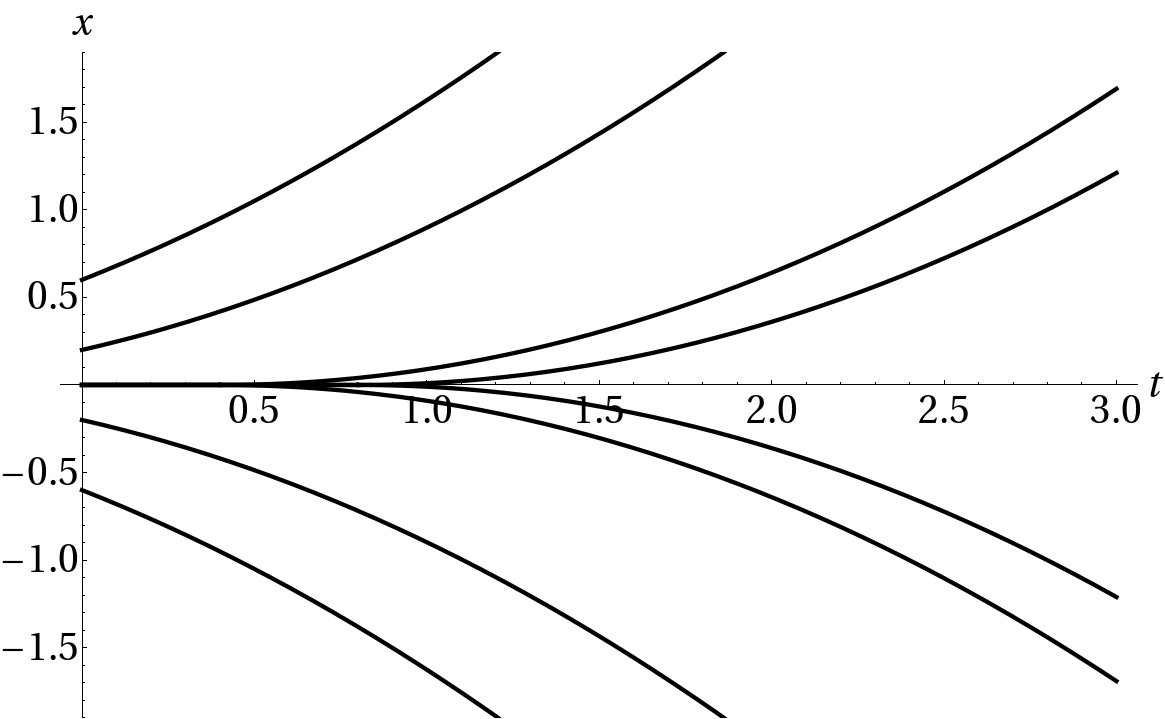
\includegraphics[width=0.44\textwidth]{ODE_Peano}
\caption{Non-uniqueness of trajectories}
\end{wrapfigure}

\hspace{15pt}Consequently, if $-1<\alpha<1$, there cannot exist a continuous flow solving the ODE: continuity fails in $x_0=0$. This also implies that non-uniqueness appears for the transport equation with discontinuous (at $0$) initial datum.

\hspace{15pt}On the contrary, for $\alpha>-1$ the drift is in the LPS class, hence all our results apply to this example and show regularization by noise in various ways. In particular, the discontinuity of the flow in the origin is removed $\omega$-wise; moreover, for $\alpha>0$ (when $b$ is H\"older continuous), we have proved path-by-path uniqueness starting from $x_0=0$. Let us also remind that pathwise uniqueness holds, starting from $0$, by~\cite{KRYROE05}. 

\end{minipage}
\\[0.2cm]

In this particular example it is possible to have an intuitive idea, ``by hands'', of what happens. If one consider the ODE without noise starting from $0$, any solution $Y$ grows near $0$ no faster than $t^{1/(1-\alpha)}$; on the contrary, the Brownian motion $W$ near $0$ grows as $t^{1/2}$ (this is false, but only for a logarithmic correction, which does not affect the intuition). Heuristically, we could say that the ``speed'' of $Y$ near $0$ which is caused by the drift is like  $t^{\alpha/(1-\alpha)}$, while the one caused by $W$ is like $t^{-1/2}$. So what we expect to happen is that the Brownian motion moves the particle immediately away from $0$, faster than the action of the drift, and this prevents the formation of non-uniqueness or singularities. At least in the one-dimensional case, this can be seen also through speed measure and scale function, see~\cite{BREIMAN}.

Notice that if $\alpha<-1$ the opposite phenomenon appears ($Y$ is faster than $W$), so that we expect ill-posedness. This is also an argument for the optimality of the LPS conditions (even if, in this case, we do not look at critical cases in LPS hypotheses). See also the counterexample~\ref{counterex}.
\end{example}

\begin{example}
We consider a similar autonomous vector field as in the previous example, but change sign:
\begin{equation*}
b(x):=-1_{0<|x|\le1}|x|^{\alpha}\hat{x}-1_{|x|>1}x.
\end{equation*}
In this case, we see that, for every initial $x_0$, there exists a unique solution $Y$ to the ODE, which reaches~$0$ in finite time and then stays in~$0$. Thus concentration appears in~$0$, so that there does not exist a Lagrangian flow (the image measure of the flow at time $t$ can have a Dirac delta in~$0$). Moreover the solution to the continuity equation concentrates in~$0$. Again our results apply when $\alpha>-1$, so these concentration phenomena disappear in the stochastic case.
\end{example}

\begin{example}
Take $d=2$ for simplicity. The following field is a combination of the previous two examples:
\begin{equation*}
b(x)=1_{x\in A}[1_{0<|x|\le1}|x|^{\alpha}\hat{x}+1_{|x|>1}x]+1_{x\in A^c}[-1_{0<|x|\le1}|x|^{\alpha}\hat{x}-1_{|x|>1}x],
\end{equation*}
where $A=\{x\in\mr^2|x_1>0\mbox{ or }(x_1=0,x_2>0)\}$. It is easy to see that, if $\alpha<1$, in the deterministic case one can build flows with discontinuity, concentration of the mass in $0$ or both; in particular, non-uniqueness holds. Again, if $\alpha>-1$, well-posedness (as in Theorem 	\ref{main thm flows}) is restored.
\end{example}

\subsection{A counterexample in the supercritical case}

\begin{example}\label{counterex}
Finally let us show that outside the LPS class there are equations and diffuse initial conditions without any solution; in particular the thesis of Theorem~\ref{2pathwise} does not hold in this case. We now consider~\eqref{SDE} on $\mr^d$,with $\sigma = 1$ and drift $b$ defined as
\begin{equation*}
b(x) :=-\beta |x|^{-2} x 1_{x\neq0} \, ,
\end{equation*}
with $\beta>1/2$. Notice that this drift is just outside the LPS class (in the sense that $|x|^{\alpha-1}x$ belongs to that class for any $\alpha>-1$). For this particular sDE, we have: for some $T>0$ and $M>0$, if $X_0$ is a random variable, independent of $W$ and uniformly distributed on $[-M,M]$, then there does not exist a weak solution, starting from $X_0$.
\end{example}

\begin{proof}
\emph{Step 1:~\eqref{SDE} does not have a weak solution for $X_0=0$ (for any $T>0$).} Notice that this does not prevent from extending Theorem~\ref{2pathwise} to this case (because the initial datum is concentrated on $0$), but it is a first step. The method is taken from~\cite{Cerny Engelbert}.

Assume, by contradiction, that $(X,W)$ is a weak solution on
$[0,T]$, i.\,e.\ there is a filtered probability
space $(\Omega,\mathcal{A},\mathcal{F}_{t},P)$, an
$\mathcal{F}_{t}$-Brownian motion $W$ in $\mathbb{R}^{d}$, an $\mathcal{F} 
_{t}$-adapted continuous process $(X_{t})_{t\geq0}$ in
$\mathbb{R}^{d}$, such that $ \int_{0}^{T} \vert b(X_{t}) \vert dt<\infty$ and, a.\,s.,
\[
X_{t}=\int_{0}^{t}b(X_{s}) ds+W_{t} \,.
\]
Hence $X$ is a continuous semimartingale, with quadratic covariation
$\left\langle X^{i},X^{j}\right\rangle _{t}=\delta_{ij}t$ between its
components. By the It\^{o} formula, we have
\begin{align*}
d\left\vert X_{t}\right\vert ^{2}  & =-2\beta1_{X_{t}\neq0}dt+2X_{t}\cdot
dW_{t}+dt\\
& =(1_{X_{t}=0}-(2\beta-1)1_{X_{t}\neq0})dt+2X_{t}\cdot dW_{t}.
\end{align*}
We now claim that
\begin{equation}
\int_{0}^{T}1_{X_{s}=0}ds=0\label{key} 
\end{equation}
holds with probability one. This implies
\[
\vert X_{t} \vert ^{2}=-(2\beta-1)\int^t_01_{X_{s}\neq0}ds+\int_{0}^{t}2X_{s}\cdot dW_{s}\,.
\]
Therefore $\vert X_{t} \vert^{2}$ is a positive local supermartingale,
null at $t=0$. This implies $\vert X_{t} \vert^{2}\equiv0$, hence $X_{t}\equiv0$. But this contradicts the fact
that $\left\langle X^{i},X^{j}\right\rangle _{t}=\delta_{ij}t$. 

It remains to prove the claim~\eqref{key}. Consider the random set $\{ t\in [
0,T] \colon X_{t}=0\}$. It is a subset of $A_{1}=\{ t\in [0,T] \colon X_{t}^{1}=0 \}$, so it is sufficient to prove that the Lebesgue measure of $A_{1}$ is zero, $P$-a.\,s.\ and this is equivalent to $P\big(\int_{0}^{T} 1_{X_{s}^{i}=0}ds=0 \big)=1$. Since $X$ is a
continuous semimartingale, with quadratic covariation $\left\langle
X^{i},X^{j}\right\rangle _{t}=\delta_{ij}t$, also $X^{1}$ is a continuous
semimartingale, with quadratic covariation $\left\langle X^{1},X^{1} 
\right\rangle _{t}=t$. Hence, by the occupation times formula (see
\cite[Chapter~VI, Corollary~1.6]{RevuzYor})
\[
\int_{0}^{T}1_{X_{s}^{1}=0}ds=\int_{\mathbb{R}}1_{a=0}L_{T}^{a}(X^{1})  da
\]
where $L_{T}^{a}( X^{1})$ is the local time at $a$ on $[
0,T]  $ of the process $X^{1}$. Hence, a.\,s.,  $\int_{0}^{T}1_{X_{s}^{1}=0}ds=0$. 

\emph{Step 2:~\eqref{SDE} does not have a weak solution starting from $X_0$ uniformly distributed on $[-M,M]$ (for some $T>0$ and $M>0$).} Again, we suppose by contradiction that there exists such a solution $X$ (associated with some filtration $\mc{G}$), on a probability space $(\Omega,\mc{A},P)$. Let $\tau$ be the first time when $X$ hits $0$ (it is a stopping time with respect to $\mc{G}$), with $\tau=\infty$ where $X$ does not hit $0$. We now claim that
\begin{equation}
P(\tau<\infty)>0 \, .\label{claim'}
\end{equation}
Assuming this, we can construct a new process $Y$, which is a weak solution to~\eqref{SDE}, starting from $Y_0=0$. This is in contradiction with Step 1. The process $Y$ is built as follows. Take $\td{\Omega}=\{\tau<\infty\}$, $\td{\mc{A}}=\{A\cap\td{\Omega}|A\in\mc{A}\}$, 
$Q= P(\td{\Omega})^{-1} P|_{\td{\mc{A}}}$, on $\td{\Omega}$ define $Y_t=X_{t+\tau}$ and $\td{W}_t=W_{t+\tau}-W_\tau$, $\mc{H}_t=\sigma\{\td{W}_s,Y_s|s\le t\}$ (this is a $\sigma$-algebra on $\td{\Omega}$).Then we observe the following facts:

\begin{itemize}
  \item $\td{W}$ is a natural Brownian motion on the space $(\td{\Omega},\mc{A},Q)$, i.\,e., for every positive integer $n$, for every $0<t_1<\ldots t_n$ and for every $f_1,\ldots f_n$ in $C_b(\mr^d)$, there holds 
  \begin{equation}
  E\Big[1_{\td{\Omega}}\prod^n_{j=1}f_j(W(t_j+\tau)-W(t_{j-1}+\tau))\Big]= P(\td{\Omega})\prod^n_{j=1}\int_{\mr^d}f_jd\mc{N}(0,(t_j-t_{j-1})I),\label{newBM}
  \end{equation}
  where $\mc{N}(m,A)$ is the Gaussian law of mean $m$ and covariance matrix $A$. This can be verified, for a general $\mc{G}$-stopping time, with a standard argument: first one proves~\eqref{newBM} when $\tau$ is a stopping time with discrete range in $[0,\infty]$, then, for the general case, one uses an approximation of $\tau$ with stopping times $\tau_k$ with discrete range such that $\tau_k\downarrow\tau$ (as $k\rightarrow\infty$) and $\{\tau=\infty\}=\{\tau_k=\infty\}$ for every $k$.
  \item $\td{W}$ is a Brownian motion with respect to the filtration $\mc{H}$, i.\,e.,\ for every $0=t_0<t_1<\ldots t_n\le s<t$ and for every $f,g_1,\ldots g_n$ in $C_b(\mr^d)$, there holds 
  \begin{equation*}
  E\Big[1_{\td{\Omega}}f(W(t+\tau)-W(s+\tau))\prod^n_{j=0}g_j(X(t_j+\tau))\Big]= \int_{\mr^d}fd\mc{N}(0,(t-s)I)E\Big[\prod^n_{j=0}g_j(X(t_j+\tau))\Big].
  \end{equation*}
  Again this can be shown by approximation (with stopping times with discrete range).
  \item $Y$ is a weak solution to~\eqref{SDE}, starting from $Y_0 = 0$. This follows immediately from
  \begin{equation*}
  X_{s'}=X_s+\int^{s'}_sb(X_r)dr+W_{s'}-W_s \,,
  \end{equation*}
  setting $s'=t+\tau$ and $s=\tau$.
\end{itemize}

It remains to prove the claim~\eqref{claim'}. We suppose by contradiction that $\tau=\infty$ a.\,s.;\ this implies that, for every $t$, $P(X_t\neq0)=1$. Then, computing $E[|X|^2]$ by the It\^o formula, we get
\begin{equation*}
\frac{d}{dt}E[|X_t|^2]=-2\beta P\{X_t\neq0\}+1=-2\beta+1<0,
\end{equation*}
hence there exists a time $t_0>0$ such that $E[|X_{t_0}|^2]<0$, which is a contradiction. This completes the proof.
\end{proof}

\begin{remark}
The restriction on $\beta$ is due to the first step. The claim~\eqref{claim'} holds in fact for the more general case $\beta>-1/2$, which can be achieved by an alternative approach.
\end{remark}

\begin{proof}[Sketch of proof]
The idea is that the symmetry properties of the drift allow to reduce the solution $X$ to the SDE to a one-dimensional Bessel process, for which we know the probability of hitting $0$. Fix $R>0$ and, for any $\eps>0$, $x$ in $B_R\setminus\bar{B}_\eps$, denote by $\tau_\eps(x)$ the exit time from the annulus $B_R\setminus\bar{B}_\eps$ of the solution $Z(x)$ to~\eqref{SDE}, starting from $x$ ($Z$ exists until $\tau_\eps(x)$ since the drift is regular in the annulus). If we prove that, for every $x\neq0$, there exist $T>0$, $\delta>0$ and $R$ large enough such that, for every $\eps>0$,
\begin{equation}
P\big( \tau_\eps(x)<T,Z(x,\tau_\eps(x))=\eps\big)>\delta \, ,\label{claim2}
\end{equation}
we have shown the claim. To prove~\eqref{claim2}, we notice that $P(\tau_\eps(x)<T,Z(x,\tau_\eps(x))=\eps)=u(0,x)$, where $u$ solves the backward parabolic PDE, on $B_R\setminus\bar{B}_\eps$,
\begin{equation*}
\partial_tu+b\cdot\nabla u+\frac12\Delta u=0 \, ,
\end{equation*}
with final and boundary conditions
\begin{equation*}
u(T,\cdot)\equiv0 \text{ in } B_R\setminus\bar{B}_\eps,\ \ u(t,\cdot) \equiv 1 \text{ on } \partial B_\eps \text{ and } 
u(t,\cdot)\equiv 1 \text{ on } \partial B_R, \text{ for all } t \in [0,T]\,.
\end{equation*}
By the symmetry properties of the drift $b$, the solution $u$ is given by $u(t,x)=v(t,|x|)$, where $v \colon [0,T]\times]\eps,R[\rightarrow\mr$ solves the PDE
\begin{equation*}
\partial_tu+\bar{b}\cdot\nabla u+\frac12\Delta u=0
\end{equation*}
for $\bar{b}(r)=-\beta|r|^{-1}1_{r\neq0}$, with final and boundary conditions
\begin{equation*}
v(T,\cdot)\equiv0,\ \ v(\cdot,\eps)\equiv1,\ \ v(\cdot,R)\equiv0 \, .
\end{equation*}
Then 
\begin{equation*}
P\big(\tau_\eps(x)<T,Z(x,\tau_\eps(x))=\eps\big)=v(0,|x|)=P\big(\sigma_\eps(|x|)<T,\xi(|x|,\sigma_\eps(|x|))=\eps\big)\,, 
\end{equation*}
where $\xi=\xi(r)$ is the one-dimensional process solution to the SDE ($B$ is a one-dimensional Brownian motion)
\begin{equation*}
d\xi=-\beta|\xi|^{-1}1_{\xi\neq0}+dB
\end{equation*}
with initial condition $\xi_0(r)=r$, and $\sigma_\eps(r)$ is the exit time of $\xi(r)$ from the interval $(\eps,R)$. Now standard tools of one-dimensional diffusion processes (speed measure and scale function, see~\cite[Chapter~16]{BREIMAN}) allow to deduce that, since $\beta>-1/2$, for every $r>0$, $\xi(r)$ hits $0$ in finite time with positive probability. This implies that, for every $r>0$, there exist $T>0$, $\delta>0$ and $R$ large enough such that, for every $\eps>0$, $P(\sigma_\eps(r)<T,\xi(r,\sigma_\eps(r))=\eps)>\delta$. We are done.
\end{proof}

\footnotesize

\begin{thebibliography}{99}                                                                                               

\bibitem{AIZENMAN78}
M. Aizenman, \textit{On vector fields as generators of flows: a counterexample to
  {N}elson's conjecture}, Ann. Math. \textbf{{\bf107}} (1978), no.~2, 287--296.

\bibitem{AMBROSIO04}
L. Ambrosio, \textit{Transport equation and {C}auchy problem for {$BV$} vector
  fields}, Invent. Math. \textbf{{\bf158}} (2004), no.~2, 227--260.

\bibitem{AMBCRI08} L. Ambrosio, G. Crippa, \textit{Existence, uniqueness, stability and differentiability properties of the flow associated to weakly differentiable vector fields, Transport equations and multi-D hyperbolic conservation laws}, Lect. Notes Unione Mat. Ital., vol. \textbf{5}, Springer, Berlin, 2008, pp. 3--57.

\bibitem {AtFl} S. Attanasio, F. Flandoli, \textit{Renormalized solutions for stochastic transport equations and the regularization by bilinear multiplication noise}, Comm. Partial Differential Equations \textbf{36} (2011), no.~8, 1455--1474.

\bibitem{BahCheDan} H. Bahouri, J.-Y. Chemin, R. Danchin, \textit{Fourier Analysis and Nonlinear Partial Differential Equations}, Springer, 2011.

\bibitem {BASCHE03}R. F. Bass, Z.-Q. Chen, \textit{Brownian motion with singular drift},
The Annals of Probab. \textbf{31} (2003), n. 2, 791-817.

\bibitem {Be}H. Beir\~{a}o Da Veiga, \textit{Remarks on the smoothness of the $L^{\infty
}(0,T;L^{3})$ solutions of the 3-D Navier-Stokes equations}, Portugal.
Math. \textbf{54} (1997), no. 4, 381--391.

\bibitem{BogDaPRoe11} V. Bogachev, G. Da Prato, M. R\"{o}ckner, \textit{Uniqueness for solutions of Fokker-Planck equations on infinite dimensional spaces}, Comm. Partial
Differential Equations \textbf{36} (2011), no. 6, 925--939.

\bibitem{BREIMAN} L. Breiman, \textit{Probability}, Corrected reprint of the 1968 original, Classics in Applied Mathematics, vol. \textbf{7}, Society for Industrial and Applied Mathematics (SIAM), Philadelphia, PA, 1992.

\bibitem{CATGUB13}
R. Catellier and M. Gubinelli, \textit{On the regularization of {ODEs} via irregular perturbations}, arXiv:1205.1735 (2012), Preprint.

\bibitem {Cerny Engelbert}A. S. Cherny, H.-J. Engelbert, \textit{Singular
stochastic differential equations}, LNM 1858. Springer-Verlag, Berlin, 2005.

\bibitem {GaKuVe}M. Chaves, K. Gaw{\c{e}}dzki, P. Horvai, A. Kupiainen, M. Vergassola,
\textit{Lagrangian dispersion in Gaussian self-similar velocity ensembles}, J.
Statist. Phys. \textbf{113} (2003), no. 5-6, 643--692.

\bibitem {ChZh}
Z.-Q. Chen, Z. Zhao, \textit{Diffusion processes and second order
elliptic operators with singular coefficients for lower order terms},
Math. Ann. \textbf{302} (1995),\ 323--357.

\bibitem{CHOGUB13}
K.~Chouk and M.~Gubinelli, \textit{Nonlinear {PDE}s with modulated dispersion},
  arXiv:1303.0822 (2013), Preprint.

\bibitem {CrDeL}G. Crippa, C. De Lellis, \textit{Estimates and regularity results for the
DiPerna-Lions flow}, J. Reine Angew. Math. \textbf{616} (2008), 15--46.

\bibitem {CoHi}R. Courant, D. Hilbert, \textit{Methods of Mathematical Physics}, Interscience
Publishers, Inc., New York, N.Y., 1953.

\bibitem{DAVIE07}
A.~M. Davie, \textit{Uniqueness of solutions of stochastic differential
  equations}, Int. Math. Res. Not. IMRN (2007), no.~24, Art. ID rnm124, 26.

\bibitem{DEBTSU11}
A.~Debussche and Y.~Tsutsumi, \textit{1{D} quintic nonlinear {S}chr\"odinger
  equation with white noise dispersion}, J. Math. Pures Appl. (9) \textbf{{\bf
  96}} (2011), no.~4, 363--376.

\bibitem {DeFlVi}F. Delarue, F. Flandoli, D. Vincenzi, \textit{Noise prevents collaps of Vlasov-Poisson point charges}, to appear in Comm. Pure Appl. Math.

\bibitem{DIPELI89}
R.~J. DiPerna and P.-L. Lions, \textit{Ordinary differential equations, transport
  theory and {S}obolev spaces}, Invent. Math. \textbf{{\bf 98}} (1989), no.~3,
  511--547.

\bibitem {SeSv}L. Escauriaza, G. Seregin, V. \v{S}ver\'{a}k, \textit{Backward uniqueness for
parabolic equations}, Arch. Ration. Mech. Anal. \textbf{169} (2003),
no. 2, 147--157.

\bibitem {FeFl} E. Fedrizzi, F. Flandoli, \textit{Noise prevents singularities in linear transport equations}, J. Funct. Anal. \textbf{264} (2013), no. 6, 1329--1354.

\bibitem{Fig08} A. Figalli, \textit{Existence and uniqueness of martingale solutions for SDEs with rough or degenerate coefficients}, J. Funct. Anal. \textbf{254}
(2008), no. 1, 109--153.

\bibitem{FLALNM}
F.~Flandoli, \textit{Random perturbation of {PDE}s and fluid dynamic models},
  Saint Flour summer school lectures 2010, Lecture Notes in Math.,
  vol.~{\bf2015}, Springer, Berlin, 2011.

\bibitem {FlGuPr4}F. Flandoli, M. Gubinelli, E. Priola, \textit{Remarks on the
stochastic transport equation with H\"{o}lder drift}, Rend. Sem. Mat. Univ.
Pol. Torino, \textbf{70}, (2012) 53--73.

\bibitem{FLAGUBPRI11}
F.~Flandoli, M.~Gubinelli, and E.~Priola, \textit{Does noise improve
  well-posedness of fluid dynamic equations?}, Stochastic partial differential
  equations and applications, Quad. Mat., vol.~{\bf25}, Dept. Math., Seconda
  Univ. Napoli, Caserta, 2010, pp.~139--155.

\bibitem{FLAGUBPRI10}
F.~Flandoli, M.~Gubinelli, and E.~Priola, \textit{Well-posedness of the transport equation by stochastic perturbation}, Invent. Math. \textbf{{\bf180}} (2010), no.~1, 1--53.

\bibitem{FLAGUBPRI10a}
F.~Flandoli, M.~Gubinelli, and E.~Priola, \textit{Full well-posedness of point vortex dynamics corresponding to   stochastic 2D Euler equations}, Stoch. Proc. Appl. \textbf{{\bf121}} (2011),
  no.~7, 1445--1463.

\bibitem {FlMaNe}F. Flandoli, M. Maurelli, M. Neklyudov, \textit{Regularization by noise of a
stochastic vector advection equation}, in preparation.

\bibitem {Ga}G. P. Galdi, \textit{An introduction to the Navier-Stokes
initial-boundary value problem}, in: Fundamental directions in mathematical
fluid mechanics, Adv. Math. Fluid Mech., Birkh\"{a}user, Basel, 2000, pp. 1-70.

\bibitem{GYOMAR01}
I. Gy\"{o}ngy, T. Mart\'{\i}nez, \textit{On stochastic differential equations with
locally unbounded drift}, Czechoslovak Math. J. \textbf{51}(126)
(2001), no. 4, 763--783.

\bibitem{KISLAD57}
A.~A. Kiselev and O.~A. Lady{\v{z}}enskaya, \emph{On the existence and
  uniqueness of the solution of the nonstationary problem for a viscous,
  incompressible fluid}, Izv. Akad. Nauk SSSR. Ser. Mat. \textbf{{\bf 21}}
  (1957), 655--680.
  
\bibitem {Kr}N. V. Krylov, \textit{Lectures on elliptic and parabolic equations in H\"older spaces}, Graduate Studies in Mathematics, \textbf{12}, AMS, Providence, RI, 1996.

\bibitem{KRYROE05}
N. V. Krylov and M. R{\"o}ckner, \textit{Strong solutions of stochastic equations
  with singular time dependent drift}, Probab. Theory Related Fields
  \textbf{{\bf131}} (2005), no.~2, 154--196.

\bibitem{KUNITA84a}
H.~Kunita, \textit{First order stochastic partial differential equations},
  Stochastic analysis ({K}atata/{K}yoto, 1982), North-Holland Math. Library,
  vol.~{\bf32}, North-Holland, 1984, pp.~249--269.

\bibitem{KUNITA84}
H.~Kunita, \textit{Stochastic differential equations and stochastic flows of
  diffeomorphisms}, \'{E}cole d'\'et\'e de probabilit\'es de {S}aint-{F}lour,
  {XII}---1982, Lecture Notes in Math., vol.~{\bf1097}, Springer, Berlin, 1984,
  pp.~143--303.

\bibitem{KUNITA90}
H.~Kunita, \textit{Stochastic flows and stochastic differential equations},
  Cambridge Studies in Advanced Mathematics, vol.~{\bf24}, Cambridge University
  Press, Cambridge, 1990.

\bibitem{LADYZ67}
O.~A. Lady{\v{z}}enskaja, \textit{Uniqueness and smoothness of generalized
  solutions of {N}avier-{S}tokes equations}, Zap. Nau\v cn. Sem. Leningrad.
  Otdel. Mat. Inst. Steklov. (LOMI) \textbf{{\bf5}} (1967), 169--185.

\bibitem{LIOPRO59}
J.-L. Lions and G.~Prodi, \textit{Un th\'eor\`eme d'existence et unicit\'e dans
  les \'equations de {N}avier-{S}tokes en dimension 2}, C. R. Acad. Sci. Paris
  \textbf{{\bf248}} (1959), 3519--3521.

\bibitem{LIONS96}
P.-L. Lions, \textit{Mathematical topics in fluid mechanics. {V}ol. 1}, Oxford
  Lecture Series in Mathematics and its Applications, vol.~{\bf3}, The
  Clarendon Press Oxford University Press, New York, 1996.

\bibitem {Ma}M. Maurelli, \textit{Wiener chaos and uniqueness for stochastic transport equation}, C. R. Math. Acad. Sci. Paris \textbf{349} (2011), no. 11-12, 669--672.

\bibitem {MoPrTh}S.-E. A. Mohammed, T. Nilssen, F. Proske, \textit{Sobolev Differentiable Stochastic Flows of SDE`s with Measurable Drift and Applications}, arXiv:1204.3867.

\bibitem {NevOli} W. Neves, C. Olivera, \textit{Wellposedness for stochastic continuity equations with Ladyzhenskaya-Prodi-Serrin condition}, arXiv:1307.6484.

\bibitem {Po}N. I. Portenko, \textit{Generalized Diffusion Processes}, Nauka, Moscow, 1982
In Russian; English translation: Amer. Math. Soc., Providence, Rhode Island, 1990.

\bibitem{PRODI59}
G.~Prodi, \textit{Un teorema di unicit\`a per le equazioni di {N}avier-{S}tokes},
  Ann. Mat. Pura Appl. (4) \textbf{{\bf 48}} (1959), 173--182.

\bibitem {RevuzYor}D. Revuz, M. Yor, \textit{Continuous Martingales and
Brownian Motion}, Springer-Verlag, Berlin, 1994.

\bibitem{SERRIN62}
J.~Serrin, \textit{On the interior regularity of weak solutions of the
  {N}avier-{S}tokes equations}, Arch. Rational Mech. Anal. \textbf{{\bf9}}
  (1962), 187--195.

\bibitem {St}W. Stannat, \textit{(Nonsymmetric) Dirichlet operators on $L^{1}$:\ existence, 
uniqueness and associated Markov processes}, Ann. Scuola
Norm. Sup. Pisa Cl. Sci. \textbf{28} (1999), 99-140.

\bibitem{StrVar} D. W. Stroock, S. R. S. Varadhan, \textit{Multidimensional diffusion processes}, Springer-Verlag, Berlin Heidelberg, 1979.

\bibitem {VERAAR12}M. Veraar, \textit{The stochastic Fubini theorem revisited}, Stochastics \textbf{84} (2012), no. 4, 543--551.

\bibitem {Ve}Y. A. Veretennikov, \textit{On strong solution and explicit formulas for solutions of stochastic integral equations}, Math. USSR Sb. \textbf{39} (1981) 387--403.

\end{thebibliography}


\end{document}
